\documentclass[a4paper, 12pt]{book}

%\usepackage[center]{titlesec}

\usepackage{amsfonts, amssymb, amsmath, amsthm, amsxtra}

\usepackage{foekfont}

\usepackage{MnSymbol}

\usepackage{pdfrender, xcolor}
%\pdfrender{StrokeColor=black,LineWidth=.4pt,TextRenderingMode=2}

\usepackage{minitoc}
\setcounter{tocdepth}{4}
\setcounter{minitocdepth}{4}
\setcounter{secnumdepth}{4}

\usepackage{graphicx}

\usepackage[english]{babel}
\usepackage[utf8]{inputenc}
%\usepackage{mathpazo}
%\usepackage{euler}
\usepackage{eucal}
\usepackage{bbm}
\usepackage{bm}
\usepackage{csquotes}
\usepackage[nottoc]{tocbibind}
\usepackage{appendix}
\usepackage{float}
\usepackage[T1]{fontenc}
\usepackage[
    left = \flqq{},% 
    right = \frqq{},% 
    leftsub = \flq{},% 
    rightsub = \frq{} %
]{dirtytalk}

\usepackage{imakeidx}
\makeindex

%\usepackage[dvipsnames]{xcolor}
\usepackage{hyperref}
    \hypersetup{
        colorlinks=true,
        linkcolor=teal,
        filecolor=pink,      
        urlcolor=teal,
        citecolor=magenta
    }
\usepackage{comment}

% You would set the PDF title, author, etc. with package options or
% \hypersetup.

\usepackage[backend=biber, style=alphabetic, sorting=nty]{biblatex}
    \addbibresource{bibliography.bib}
\renewbibmacro{in:}{}

\raggedbottom

\usepackage{mathrsfs}
\usepackage{mathtools} 
\mathtoolsset{showonlyrefs}
%\usepackage{amsthm}
\renewcommand\qedsymbol{$\blacksquare$}
\usepackage{tikz-cd}
\tikzcdset{scale cd/.style={every label/.append style={scale=#1},
    cells={nodes={scale=#1}}}}
\usepackage{tikz}
\usepackage{setspace}
\usepackage[version=3]{mhchem}
\parskip=0.1in
\usepackage[margin=25mm]{geometry}

\usepackage{listings, lstautogobble}
\lstset{
	language=matlab,
	basicstyle=\scriptsize\ttfamily,
	commentstyle=\ttfamily\itshape\color{gray},
	stringstyle=\ttfamily,
	showstringspaces=false,
	breaklines=true,
	frameround=ffff,
	frame=single,
	rulecolor=\color{black},
	autogobble=true
}

\usepackage{todonotes,tocloft,xpatch,hyperref}

% This is based on classicthesis chapter definition
\let\oldsec=\section
\renewcommand*{\section}{\secdef{\Sec}{\SecS}}
\newcommand\SecS[1]{\oldsec*{#1}}%
\newcommand\Sec[2][]{\oldsec[\texorpdfstring{#1}{#1}]{#2}}%

\newcounter{istodo}[section]

% http://tex.stackexchange.com/a/61267/11984
\makeatletter
%\xapptocmd{\Sec}{\addtocontents{tdo}{\protect\todoline{\thesection}{#1}{}}}{}{}
\newcommand{\todoline}[1]{\@ifnextchar\Endoftdo{}{\@todoline{#1}}}
\newcommand{\@todoline}[3]{%
	\@ifnextchar\todoline{}
	{\contentsline{section}{\numberline{#1}#2}{#3}{}{}}%
}
\let\l@todo\l@subsection
\newcommand{\Endoftdo}{}

\AtEndDocument{\addtocontents{tdo}{\string\Endoftdo}}
\makeatother

\usepackage{lipsum}

%   Reduce the margin of the summary:
\def\changemargin#1#2{\list{}{\rightmargin#2\leftmargin#1}\item[]}
\let\endchangemargin=\endlist 

%   Generate the environment for the abstract:
\newcommand\summaryname{Abstract}
\newenvironment{abstract}%
    {\small\begin{center}%
    \bfseries{\summaryname} \end{center}}

\newtheorem{theorem}{Theorem}[section]
    \numberwithin{theorem}{subsection}
\newtheorem{proposition}{Proposition}[section]
    \numberwithin{proposition}{subsection}
\newtheorem{lemma}{Lemma}[section]
    \numberwithin{lemma}{subsection}
\newtheorem{claim}{Claim}[section]
    \numberwithin{claim}{subsection}
\newtheorem{question}{Question}[section]
    \numberwithin{question}{subsection}

\theoremstyle{definition}
    \newtheorem{definition}{Definition}[section]
        \numberwithin{definition}{subsection}

\theoremstyle{remark}
    \newtheorem{remark}{Remark}[section]
        \numberwithin{remark}{subsection}
    \newtheorem{example}{Example}[section]
        \numberwithin{example}{subsection}    
    \newtheorem{convention}{Convention}[section]
        \numberwithin{convention}{subsection}
    \newtheorem{corollary}{Corollary}[section]
        \numberwithin{corollary}{subsection}

\numberwithin{equation}{chapter}

\setcounter{section}{-1}

\renewcommand{\implies}{\Rightarrow}
\renewcommand{\cong}{\simeq}
\newcommand{\codim}{\operatorname{codim}}
\newcommand{\ladjoint}{\dashv}
\newcommand{\radjoint}{\vdash}
\newcommand{\<}{\langle}
\renewcommand{\>}{\rangle}
\newcommand\bra[2][]{#1\langle {#2} #1\rvert}
\newcommand\ket[2][]{#1\lvert {#2} #1\rangle}
\newcommand\abs[2][]{#1\left\lvert {#2} #1\right\rvert}
\newcommand\norm[2][]{#1\left\| {#2} #1\right\|}
\newcommand\order[2][]{#1\: \mathbf{:} \: {#2} #1 \: \mathbf{:} \:}
\newcommand{\ndiv}{\hspace{-2pt}\not|\hspace{5pt}}
\newcommand{\cond}{\blacktriangle}
\newcommand{\decond}{\triangle}
\newcommand{\solid}{\blacksquare}
\newcommand{\ot}{\leftarrow}
\renewcommand{\-}{\text{-}}
\renewcommand{\mapsto}{\leadsto}
\renewcommand{\leq}{\leqslant}
\renewcommand{\geq}{\geqslant}
\renewcommand{\setminus}{\smallsetminus}
\newcommand{\punc}{\overset{\circ}}
\renewcommand{\div}{\operatorname{div}}
\newcommand{\grad}{\operatorname{grad}}
\newcommand{\curl}{\operatorname{curl}}
\makeatletter
\DeclareRobustCommand{\cev}[1]{%
  {\mathpalette\do@cev{#1}}%
}
\newcommand{\do@cev}[2]{%
  \vbox{\offinterlineskip
    \sbox\z@{$\m@th#1 x$}%
    \ialign{##\cr
      \hidewidth\reflectbox{$\m@th#1\vec{}\mkern4mu$}\hidewidth\cr
      \noalign{\kern-\ht\z@}
      $\m@th#1#2$\cr
    }%
  }%
}
\makeatother

\newcommand{\N}{\mathbb{N}}
\newcommand{\Z}{\mathbb{Z}}
\newcommand{\Q}{\mathbb{Q}}
\newcommand{\R}{\mathbb{R}}
\newcommand{\bbC}{\mathbb{C}}
\newcommand{\bbK}{\mathbb{K}}
\NewDocumentCommand{\x}{e{_^}}{%
  \mathbin{\mathop{\times}\displaylimits
    \IfValueT{#1}{_{#1}}
    \IfValueT{#2}{^{#2}}
  }%
}
\NewDocumentCommand{\pushout}{e{_^}}{%
  \mathbin{\mathop{\sqcup}\displaylimits
    \IfValueT{#1}{_{#1}}
    \IfValueT{#2}{^{#2}}
  }%
}
\newcommand{\simpleroots}{\mathbb{I}}
\newcommand{\supp}{\operatorname{supp}}
\newcommand{\domain}{\operatorname{dom}}
\newcommand{\codomain}{\operatorname{codom}}
\newcommand{\im}{\operatorname{im}}
\newcommand{\coim}{\operatorname{coim}}
\newcommand{\coker}{\operatorname{coker}}
\newcommand{\id}{\mathrm{id}}
\newcommand{\chara}{\operatorname{char}}
\newcommand{\trdeg}{\operatorname{trdeg}}
\newcommand{\rank}{\operatorname{rank}}
\newcommand{\trace}{\operatorname{tr}}
\newcommand{\quantumdet}{\operatorname{qdet}}
\newcommand{\skdet}{\operatorname{skdet}}
\newcommand{\quasidet}{\operatorname{quasidet}}
\newcommand{\length}{\operatorname{length}}
\newcommand{\height}{\operatorname{ht}}
\renewcommand{\span}{\operatorname{span}}
\newcommand{\e}{\epsilon}
\newcommand{\p}{\mathfrak{p}}
\newcommand{\q}{\mathfrak{q}}
\newcommand{\m}{\mathfrak{m}}
\newcommand{\n}{\mathfrak{n}}
\newcommand{\calF}{\mathcal{F}}
\newcommand{\calG}{\mathcal{G}}
\newcommand{\calO}{\mathcal{O}}
\newcommand{\F}{\mathbb{F}}
\DeclareMathOperator{\lcm}{lcm}
\newcommand{\gr}{\operatorname{gr}}
\newcommand{\vol}{\mathrm{vol}}
\newcommand{\ord}{\operatorname{ord}}
\newcommand{\projdim}{\operatorname{proj.dim}}
\newcommand{\injdim}{\operatorname{inj.dim}}
\newcommand{\flatdim}{\operatorname{flat.dim}}
\newcommand{\globdim}{\operatorname{glob.dim}}
\renewcommand{\Re}{\operatorname{Re}}
\renewcommand{\Im}{\operatorname{Im}}
\newcommand{\sgn}{\operatorname{sgn}}
\newcommand{\coad}{\operatorname{coad}}
\newcommand{\ch}{\operatorname{ch}} %characters of representations
\newcommand{\dist}{\operatorname{dist}} %distance

\newcommand{\Ad}{\mathrm{Ad}}
\newcommand{\GL}{\mathrm{GL}}
\newcommand{\SL}{\mathrm{SL}}
\newcommand{\PGL}{\mathrm{PGL}}
\newcommand{\PSL}{\mathrm{PSL}}
\newcommand{\Sp}{\mathrm{Sp}}
\newcommand{\GSp}{\mathrm{GSp}}
\newcommand{\GSpin}{\mathrm{GSpin}}
\newcommand{\rmO}{\mathrm{O}}
\newcommand{\SO}{\mathrm{SO}}
\newcommand{\SU}{\mathrm{SU}}
\newcommand{\rmU}{\mathrm{U}}
\newcommand{\rmH}{\mathrm{H}}
\newcommand{\rmY}{\mathrm{Y}}
\newcommand{\rmu}{\mathrm{u}}
\newcommand{\rmV}{\mathrm{V}}
\newcommand{\gl}{\mathfrak{gl}}
\renewcommand{\sl}{\mathfrak{sl}}
\newcommand{\diag}{\mathfrak{diag}}
\newcommand{\pgl}{\mathfrak{pgl}}
\newcommand{\psl}{\mathfrak{psl}}
\newcommand{\fraksp}{\mathfrak{sp}}
\newcommand{\gsp}{\mathfrak{gsp}}
\newcommand{\gspin}{\mathfrak{gspin}}
\newcommand{\frako}{\mathfrak{o}}
\newcommand{\so}{\mathfrak{so}}
\newcommand{\su}{\mathfrak{su}}
\newcommand{\Spec}{\operatorname{Spec}}
\newcommand{\Spf}{\operatorname{Spf}}
\newcommand{\Spm}{\operatorname{Spm}}
\newcommand{\Spv}{\operatorname{Spv}}
\newcommand{\Spa}{\operatorname{Spa}}
\newcommand{\Spd}{\operatorname{Spd}}
\newcommand{\Proj}{\operatorname{Proj}}
\newcommand{\Gr}{\mathrm{Gr}}
\newcommand{\Hecke}{\mathrm{Hecke}}
\newcommand{\Sht}{\mathrm{Sht}}
\newcommand{\Quot}{\mathrm{Quot}}
\newcommand{\Hilb}{\mathrm{Hilb}}
\newcommand{\Pic}{\mathrm{Pic}}
\newcommand{\Div}{\mathrm{Div}}
\newcommand{\Jac}{\mathrm{Jac}}
\newcommand{\Alb}{\mathrm{Alb}} %albanese variety
\newcommand{\Bun}{\mathrm{Bun}}
\newcommand{\loopspace}{\mathbf{\Omega}}
\newcommand{\suspension}{\mathbf{\Sigma}}
\newcommand{\tangent}{\mathrm{T}} %tangent space
\newcommand{\Eig}{\mathrm{Eig}}
\newcommand{\Cox}{\mathrm{Cox}} %coxeter functors
\newcommand{\rmK}{\mathrm{K}} %Killing form
\newcommand{\km}{\mathfrak{km}} %kac-moody algebras
\newcommand{\Dyn}{\mathrm{Dyn}} %associated Dynkin quivers
\newcommand{\Car}{\mathrm{Car}} %cartan matrices of finite quivers
\newcommand{\uce}{\mathfrak{uce}} %universal central extension of lie algebras

\newcommand{\Ring}{\mathrm{Ring}}
\newcommand{\Cring}{\mathrm{CRing}}
\newcommand{\Bool}{\mathrm{Bool}} %boolean algebras
\newcommand{\Alg}{\mathrm{Alg}}
\newcommand{\Leib}{\mathrm{Leib}} %leibniz algebras
\newcommand{\Fld}{\mathrm{Fld}}
\newcommand{\Sets}{\mathrm{Sets}}
\newcommand{\Equiv}{\mathrm{Equiv}} %equivalence relations
\newcommand{\Cat}{\mathrm{Cat}}
\newcommand{\Grp}{\mathrm{Grp}}
\newcommand{\Ab}{\mathrm{Ab}}
\newcommand{\Sch}{\mathrm{Sch}}
\newcommand{\Coh}{\mathrm{Coh}}
\newcommand{\QCoh}{\mathrm{QCoh}}
\newcommand{\Perf}{\mathrm{Perf}} %perfect complexes
\newcommand{\Sing}{\mathrm{Sing}} %singularity categories
\newcommand{\Desc}{\mathrm{Desc}}
\newcommand{\Sh}{\mathrm{Sh}}
\newcommand{\Psh}{\mathrm{PSh}}
\newcommand{\Fib}{\mathrm{Fib}}
\renewcommand{\mod}{\-\mathrm{mod}}
\newcommand{\comod}{\-\mathrm{comod}}
\newcommand{\bimod}{\-\mathrm{bimod}}
\newcommand{\Vect}{\mathrm{Vect}}
\newcommand{\Rep}{\mathrm{Rep}}
\newcommand{\Grpd}{\mathrm{Grpd}}
\newcommand{\Arr}{\mathrm{Arr}}
\newcommand{\Esp}{\mathrm{Esp}}
\newcommand{\Ob}{\mathrm{Ob}}
\newcommand{\Mor}{\mathrm{Mor}}
\newcommand{\Mfd}{\mathrm{Mfd}}
\newcommand{\Riem}{\mathrm{Riem}}
\newcommand{\RS}{\mathrm{RS}}
\newcommand{\LRS}{\mathrm{LRS}}
\newcommand{\TRS}{\mathrm{TRS}}
\newcommand{\TLRS}{\mathrm{TLRS}}
\newcommand{\LVRS}{\mathrm{LVRS}}
\newcommand{\LBRS}{\mathrm{LBRS}}
\newcommand{\Spc}{\mathrm{Spc}}
\newcommand{\Top}{\mathrm{Top}}
\newcommand{\Topos}{\mathrm{Topos}}
\newcommand{\Nil}{\operatorname{Nil}}
\newcommand{\Rad}{\operatorname{Rad}}
\newcommand{\Stk}{\mathrm{Stk}}
\newcommand{\Pre}{\mathrm{Pre}}
\newcommand{\simp}{\mathbf{\Delta}}
\newcommand{\Res}{\mathrm{Res}}
\newcommand{\Ind}{\mathrm{Ind}}
\newcommand{\Pro}{\mathrm{Pro}}
\newcommand{\Mon}{\mathrm{Mon}}
\newcommand{\Comm}{\mathrm{Comm}}
\newcommand{\Fin}{\mathrm{Fin}}
\newcommand{\Assoc}{\mathrm{Assoc}}
\newcommand{\Semi}{\mathrm{Semi}}
\newcommand{\Co}{\mathrm{Co}}
\newcommand{\Loc}{\mathrm{Loc}}
\newcommand{\Ringed}{\mathrm{Ringed}}
\newcommand{\Haus}{\mathrm{Haus}} %hausdorff spaces
\newcommand{\Comp}{\mathrm{Comp}} %compact hausdorff spaces
\newcommand{\Stone}{\mathrm{Stone}} %stone spaces
\newcommand{\Extr}{\mathrm{Extr}} %extremely disconnected spaces
\newcommand{\Ouv}{\mathrm{Ouv}}
\newcommand{\Str}{\mathrm{Str}}
\newcommand{\Func}{\mathrm{Func}}
\newcommand{\Crys}{\mathrm{Crys}}
\newcommand{\LocSys}{\mathrm{LocSys}}
\newcommand{\Sieves}{\mathrm{Sieves}}
\newcommand{\pt}{\mathrm{pt}}
\newcommand{\Graphs}{\mathrm{Graphs}}
\newcommand{\Lie}{\mathrm{Lie}}
\newcommand{\Env}{\mathrm{Env}}
\newcommand{\Ho}{\mathrm{Ho}}
\newcommand{\rmD}{\mathrm{D}}
\newcommand{\Cov}{\mathrm{Cov}}
\newcommand{\Frames}{\mathrm{Frames}}
\newcommand{\Locales}{\mathrm{Locales}}
\newcommand{\Span}{\mathrm{Span}}
\newcommand{\Corr}{\mathrm{Corr}}
\newcommand{\Monad}{\mathrm{Monad}}
\newcommand{\Var}{\mathrm{Var}}
\newcommand{\sfN}{\mathrm{N}} %nerve
\newcommand{\Diam}{\mathrm{Diam}} %diamonds
\newcommand{\co}{\mathrm{co}}
\newcommand{\ev}{\mathrm{ev}}
\newcommand{\bi}{\mathrm{bi}}
\newcommand{\Nat}{\mathrm{Nat}}
\newcommand{\Hopf}{\mathrm{Hopf}}
\newcommand{\Dmod}{\mathrm{D}\mod}
\newcommand{\Perv}{\mathrm{Perv}}
\newcommand{\Sph}{\mathrm{Sph}}
\newcommand{\Moduli}{\mathrm{Moduli}}
\newcommand{\Pseudo}{\mathrm{Pseudo}}
\newcommand{\Lax}{\mathrm{Lax}}
\newcommand{\Strict}{\mathrm{Strict}}
\newcommand{\Opd}{\mathrm{Opd}} %operads
\newcommand{\Shv}{\mathrm{Shv}}
\newcommand{\Char}{\mathrm{Char}} %CharShv = character sheaves
\newcommand{\Huber}{\mathrm{Huber}}
\newcommand{\Tate}{\mathrm{Tate}}
\newcommand{\Affd}{\mathrm{Affd}} %affinoid algebras
\newcommand{\Adic}{\mathrm{Adic}} %adic spaces
\newcommand{\Rig}{\mathrm{Rig}}
\newcommand{\An}{\mathrm{An}}
\newcommand{\Perfd}{\mathrm{Perfd}} %perfectoid spaces
\newcommand{\Sub}{\mathrm{Sub}} %subobjects
\newcommand{\Ideals}{\mathrm{Ideals}}
\newcommand{\Isoc}{\mathrm{Isoc}} %isocrystals
\newcommand{\Ban}{\mathrm{Ban}} %Banach spaces
\newcommand{\Fre}{\mathrm{Fr\acute{e}}} %Frechet spaces
\newcommand{\Ch}{\mathrm{Ch}} %chain complexes
\newcommand{\Pure}{\mathrm{Pure}}
\newcommand{\Mixed}{\mathrm{Mixed}}
\newcommand{\Hodge}{\mathrm{Hodge}} %Hodge structures
\newcommand{\Mot}{\mathrm{Mot}} %motives
\newcommand{\KL}{\mathrm{KL}} %category of Kazhdan-Lusztig modules
\newcommand{\Pres}{\mathrm{Pr}} %presentable categories
\newcommand{\Noohi}{\mathrm{Noohi}} %category of Noohi groups
\newcommand{\Inf}{\mathrm{Inf}}
\newcommand{\LPar}{\mathrm{LPar}} %Langlands parameters
\newcommand{\ORig}{\mathrm{ORig}} %overconvergent sites
\newcommand{\Quiv}{\mathrm{Quiv}} %quivers
\newcommand{\Def}{\mathrm{Def}} %deformation functors
\newcommand{\Root}{\mathrm{Root}}
\newcommand{\gRep}{\mathrm{gRep}}
\newcommand{\Higgs}{\mathrm{Higgs}}
\newcommand{\BGG}{\mathrm{BGG}}
\newcommand{\Poiss}{\mathrm{Poiss}}
\newcommand{\Fact}{\mathrm{Fact}} %factorisation
\newcommand{\Chr}{\mathrm{Chr}} %chiral
\newcommand{\Smooth}{\mathrm{Sm}}

\newcommand{\Aut}{\mathrm{Aut}}
\newcommand{\Inn}{\mathrm{Inn}}
\newcommand{\Out}{\mathrm{Out}}
\newcommand{\der}{\mathfrak{der}} %derivations on Lie algebras
\newcommand{\frakend}{\mathfrak{end}}
\newcommand{\aut}{\mathfrak{aut}}
\newcommand{\inn}{\mathfrak{inn}} %inner derivations
\newcommand{\out}{\mathfrak{out}} %outer derivations
\newcommand{\Stab}{\mathrm{Stab}}
\newcommand{\Cent}{\mathrm{Cent}}
\newcommand{\Norm}{\mathrm{Norm}}
\newcommand{\Core}{\mathrm{Core}}
\newcommand{\cent}{\mathfrak{cent}}
\newcommand{\core}{\mathfrak{core}}
\newcommand{\Transporter}{\mathrm{Transp}} %transporter between two subsets of a group
\newcommand{\Conj}{\mathrm{Conj}}
\newcommand{\Diag}{\mathrm{Diag}}
\newcommand{\Gal}{\mathrm{Gal}}
\newcommand{\bfG}{\mathbf{G}} %absolute Galois group
\newcommand{\Frac}{\mathrm{Frac}}
\newcommand{\Ann}{\mathrm{Ann}}
\newcommand{\Val}{\mathrm{Val}}
\newcommand{\Chow}{\mathrm{Chow}}
\newcommand{\Sym}{\mathrm{Sym}}
\newcommand{\End}{\mathrm{End}}
\newcommand{\Mat}{\mathrm{Mat}}
\newcommand{\Diff}{\mathrm{Diff}}
\newcommand{\Autom}{\mathrm{Autom}}
\newcommand{\Artin}{\mathrm{Artin}} %artin maps
\newcommand{\sk}{\mathrm{sk}} %skeleton of a category
\newcommand{\eqv}{\mathrm{eqv}} %functor that maps groups $G$ to $G$-sets
\newcommand{\Inert}{\mathrm{Inert}}
\newcommand{\Fil}{\mathrm{Fil}}
\newcommand{\prim}{\mathfrak{prim}}
\newcommand{\Nerve}{\mathrm{N}}
\newcommand{\Hol}{\mathrm{Hol}} %holomorphic functions %holonomy groups
\newcommand{\Bi}{\mathrm{Bi}} %Bi for biholomorphic functions
\newcommand{\chev}{\operatorname{chev}}
\newcommand{\bfLie}{\mathbf{Lie}} %non-reduced lie algebra associated to generalised cartan matrices
\newcommand{\frakLie}{\mathfrak{Lie}} %reduced lie algebra associated to generalised cartan matrices
\newcommand{\frakChev}{\mathfrak{Chev}} 
\newcommand{\Rees}{\operatorname{Rees}}
\newcommand{\Dr}{\mathrm{Dr}} %Drinfeld's quantum double 
\newcommand{\frakDr}{\mathfrak{Dr}} %classical double of lie bialgebras
\newcommand{\Tot}{\operatorname{Tot}} %total complexes

\renewcommand{\projlim}{\varprojlim}
\newcommand{\indlim}{\varinjlim}
%\newcommand{\colim}{\operatorname{colim}}
%\renewcommand{\lim}{\operatorname{lim}}
\newcommand{\toto}{\rightrightarrows}
%\newcommand{\tensor}{\otimes}
\NewDocumentCommand{\tensor}{e{_^}}{%
  \mathbin{\mathop{\otimes}\displaylimits
    \IfValueT{#1}{_{#1}}
    \IfValueT{#2}{^{#2}}
  }%
}
\NewDocumentCommand{\singtensor}{e{_^}}{%
  \mathbin{\mathop{\odot}\displaylimits
    \IfValueT{#1}{_{#1}}
    \IfValueT{#2}{^{#2}}
  }%
}
\NewDocumentCommand{\hattensor}{e{_^}}{%
  \mathbin{\mathop{\hat{\otimes}}\displaylimits
    \IfValueT{#1}{_{#1}}
    \IfValueT{#2}{^{#2}}
  }%
}
\NewDocumentCommand{\brevetensor}{e{_^}}{%
  \mathbin{\mathop{\breve{\otimes}}\displaylimits
    \IfValueT{#1}{_{#1}}
    \IfValueT{#2}{^{#2}}
  }%
}
\NewDocumentCommand{\semidirect}{e{_^}}{%
  \mathbin{\mathop{\rtimes}\displaylimits
    \IfValueT{#1}{_{#1}}
    \IfValueT{#2}{^{#2}}
  }%
}
\newcommand{\eq}{\operatorname{eq}}
\newcommand{\coeq}{\operatorname{coeq}}
\newcommand{\Hom}{\mathrm{Hom}}
\newcommand{\Maps}{\mathrm{Maps}}
\newcommand{\Tor}{\mathrm{Tor}}
\newcommand{\Ext}{\mathrm{Ext}}
\newcommand{\Isom}{\mathrm{Isom}}
\newcommand{\stalk}{\mathrm{stalk}}
\newcommand{\RKE}{\operatorname{RKE}}
\newcommand{\LKE}{\operatorname{LKE}}
\newcommand{\oblv}{\mathrm{oblv}}
\newcommand{\const}{\mathrm{const}}
\newcommand{\free}{\mathrm{free}}
\newcommand{\adrep}{\mathrm{ad}} %adjoint representation
\newcommand{\NL}{\mathbb{NL}} %naive cotangent complex
\newcommand{\pr}{\operatorname{pr}}
\newcommand{\Der}{\mathrm{Der}}
\newcommand{\Frob}{\mathrm{Fr}} %Frobenius
\newcommand{\frob}{\mathrm{f}} %trace of Frobenius
\newcommand{\bfpt}{\mathbf{pt}}
\newcommand{\bfloc}{\mathbf{loc}}
\DeclareMathAlphabet{\mymathbb}{U}{BOONDOX-ds}{m}{n}
\newcommand{\0}{\mymathbb{0}}
\newcommand{\1}{\mathbbm{1}}
\newcommand{\2}{\mathbbm{2}}
\newcommand{\Jet}{\mathrm{Jet}}
\newcommand{\Split}{\mathrm{Split}}
\newcommand{\Sq}{\mathrm{Sq}}
\newcommand{\Zero}{\mathrm{Z}}
\newcommand{\SqZ}{\Sq\Zero}
\newcommand{\lie}{\mathfrak{lie}}
\newcommand{\y}{\mathrm{y}} %yoneda
\newcommand{\Sm}{\mathrm{Sm}}
\newcommand{\AJ}{\phi} %abel-jacobi map
\newcommand{\act}{\mathrm{act}}
\newcommand{\ram}{\mathrm{ram}} %ramification index
\newcommand{\inv}{\mathrm{inv}}
\newcommand{\Spr}{\mathrm{Spr}} %the Springer map/sheaf
\newcommand{\Refl}{\mathrm{Refl}} %reflection functor]
\newcommand{\HH}{\mathrm{HH}} %Hochschild (co)homology
\newcommand{\HC}{\mathrm{HC}} %cyclic (co)homology
\newcommand{\Poinc}{\mathrm{Poinc}}
\newcommand{\Simpson}{\mathrm{Simpson}}
\newcommand{\Section}{\operatorname{Sect}}
\newcommand{\Ran}{\operatorname{Ran}} %Ran space
\newcommand{\quantumfields}{\operatorname{QFld}}

\newcommand{\bbU}{\mathbb{U}}
\newcommand{\V}{\mathbb{V}}
\newcommand{\W}{\mathbb{W}}
\newcommand{\calU}{\mathcal{U}}
\newcommand{\calW}{\mathcal{W}}
\newcommand{\rmI}{\mathrm{I}} %augmentation ideal
\newcommand{\bfV}{\mathbf{V}}
\newcommand{\C}{\mathcal{C}}
\newcommand{\D}{\mathcal{D}}
\newcommand{\scrD}{\mathscr{D}}
\newcommand{\T}{\mathscr{T}} %Tate modules
\newcommand{\calM}{\mathcal{M}}
\newcommand{\calN}{\mathcal{N}}
\newcommand{\calP}{\mathcal{P}}
\newcommand{\calQ}{\mathcal{Q}}
\newcommand{\A}{\mathbb{A}}
\renewcommand{\P}{\mathbb{P}}
\newcommand{\calL}{\mathcal{L}}
\newcommand{\scrL}{\mathscr{L}}
\newcommand{\E}{\mathcal{E}}
\renewcommand{\H}{\mathbf{H}}
\newcommand{\scrS}{\mathscr{S}}
\newcommand{\calX}{\mathcal{X}}
\newcommand{\calY}{\mathcal{Y}}
\newcommand{\calZ}{\mathcal{Z}}
\newcommand{\calS}{\mathcal{S}}
\newcommand{\calR}{\mathcal{R}}
\newcommand{\scrX}{\mathscr{X}}
\newcommand{\scrY}{\mathscr{Y}}
\newcommand{\scrZ}{\mathscr{Z}}
\newcommand{\calA}{\mathcal{A}}
\newcommand{\calB}{\mathcal{B}}
\renewcommand{\S}{\mathcal{S}}
\newcommand{\B}{\mathbb{B}}
\newcommand{\bbD}{\mathbb{D}}
\newcommand{\G}{\mathbb{G}}
\newcommand{\horn}{\mathbf{\Lambda}}
\renewcommand{\L}{\mathbb{L}}
\renewcommand{\a}{\mathfrak{a}}
\renewcommand{\b}{\mathfrak{b}}
\renewcommand{\c}{\mathfrak{c}}
\renewcommand{\d}{\mathfrak{d}}
\renewcommand{\t}{\mathfrak{t}}
\renewcommand{\r}{\mathfrak{r}}
\newcommand{\fraku}{\mathfrak{u}}
\newcommand{\fraky}{\mathfrak{y}}
\newcommand{\frakv}{\mathfrak{v}}
\newcommand{\frakw}{\mathfrak{w}}
\newcommand{\frake}{\mathfrak{e}}
\newcommand{\bbX}{\mathbb{X}}
\newcommand{\frakG}{\mathfrak{G}}
\newcommand{\frakH}{\mathfrak{H}}
\newcommand{\frakE}{\mathfrak{E}}
\newcommand{\frakF}{\mathfrak{F}}
\newcommand{\g}{\mathfrak{g}}
\newcommand{\frakl}{\mathfrak{l}}
\newcommand{\h}{\mathfrak{h}}
\renewcommand{\k}{\mathfrak{k}}
\newcommand{\z}{\mathfrak{z}}
\newcommand{\fraki}{\mathfrak{i}}
\newcommand{\frakj}{\mathfrak{j}}
\newcommand{\del}{\partial}
\newcommand{\bbE}{\mathbb{E}}
\newcommand{\scrO}{\mathscr{O}}
\newcommand{\bbO}{\mathbb{O}}
\newcommand{\scrA}{\mathscr{A}}
\newcommand{\scrB}{\mathscr{B}}
\newcommand{\scrE}{\mathscr{E}}
\newcommand{\scrF}{\mathscr{F}}
\newcommand{\scrG}{\mathscr{G}}
\newcommand{\scrM}{\mathscr{M}}
\newcommand{\scrN}{\mathscr{N}}
\newcommand{\scrP}{\mathscr{P}}
\newcommand{\frakS}{\mathfrak{S}}
\newcommand{\frakT}{\mathfrak{T}}
\newcommand{\calI}{\mathcal{I}}
\newcommand{\calJ}{\mathcal{J}}
\newcommand{\scrI}{\mathscr{I}}
\newcommand{\scrJ}{\mathscr{J}}
\newcommand{\scrK}{\mathscr{K}}
\newcommand{\calK}{\mathcal{K}}
\newcommand{\scrV}{\mathscr{V}}
\newcommand{\scrW}{\mathscr{W}}
\newcommand{\bbS}{\mathbb{S}}
\newcommand{\scrH}{\mathscr{H}}
\newcommand{\bfA}{\mathbf{A}}
\newcommand{\bfB}{\mathbf{B}}
\newcommand{\bfC}{\mathbf{C}}
\renewcommand{\O}{\mathbb{O}}
\newcommand{\calV}{\mathcal{V}}
\newcommand{\scrR}{\mathscr{R}} %radical
\newcommand{\sfR}{\mathsf{R}} %quantum R-matrices
\newcommand{\sfr}{\mathsf{r}} %classical R-matrices
\newcommand{\rmZ}{\mathrm{Z}} %centre of algebra
\newcommand{\rmC}{\mathrm{C}} %centralisers in algebras
\newcommand{\bfGamma}{\mathbf{\Gamma}}
\newcommand{\scrU}{\mathscr{U}}
\newcommand{\rmW}{\mathrm{W}} %Weil group
\newcommand{\frakM}{\mathfrak{M}}
\newcommand{\frakN}{\mathfrak{N}}
\newcommand{\frakB}{\mathfrak{B}}
\newcommand{\frakX}{\mathfrak{X}}
\newcommand{\frakY}{\mathfrak{Y}}
\newcommand{\frakZ}{\mathfrak{Z}}
\newcommand{\frakU}{\mathfrak{U}}
\newcommand{\frakR}{\mathfrak{R}}
\newcommand{\frakP}{\mathfrak{P}}
\newcommand{\frakQ}{\mathfrak{Q}}
\newcommand{\sfX}{\mathsf{X}}
\newcommand{\sfY}{\mathsf{Y}}
\newcommand{\sfZ}{\mathsf{Z}}
\newcommand{\sfS}{\mathsf{S}}
\newcommand{\sfT}{\mathsf{T}}
\newcommand{\sfOmega}{\mathsf{\Omega}} %drinfeld p-adic upper-half plane
\newcommand{\rmA}{\mathrm{A}}
\newcommand{\rmB}{\mathrm{B}}
\newcommand{\calT}{\mathcal{T}}
\newcommand{\sfA}{\mathsf{A}}
\newcommand{\sfB}{\mathsf{B}}
\newcommand{\sfC}{\mathsf{C}}
\newcommand{\sfD}{\mathsf{D}}
\newcommand{\sfE}{\mathsf{E}}
\newcommand{\sfF}{\mathsf{F}}
\newcommand{\sfG}{\mathsf{G}}
\newcommand{\frakL}{\mathfrak{L}}
\newcommand{\K}{\mathrm{K}}
\newcommand{\rmT}{\mathrm{T}}
\newcommand{\bfv}{\mathbf{v}}
\newcommand{\bfg}{\mathbf{g}}
\newcommand{\frakV}{\mathfrak{V}}
\newcommand{\bfn}{\mathbf{n}}
\renewcommand{\o}{\mathfrak{o}}
\newcommand{\standard}{\Delta}
\newcommand{\costandard}{\nabla}
\newcommand{\simple}{\bar{\Delta}}
\newcommand{\cosimple}{\bar{\nabla}}
\newcommand{\qsimple}{\bar{ \mathbf{ \Delta } }}
\newcommand{\qcosimple}{\bar{ \mathbf{ \nabla } }}
\newcommand{\qstandard}{\mathbf{ \Delta }}
\newcommand{\qcostandard}{\mathbf{ \nabla }}
\newcommand{\frakD}{\mathfrak{D}}
\newcommand{\rmi}{\mathrm{i}}
\newcommand{\bfH}{\mathbf{H}}
\newcommand{\bfX}{\mathbf{X}}
\newcommand{\coxeter}{\mathrm{h}}

\newcommand{\aff}{\mathrm{aff}}
\newcommand{\ft}{\mathrm{ft}} %finite type
\newcommand{\fp}{\mathrm{fp}} %finite presentation
\newcommand{\fr}{\mathrm{fr}} %free
\newcommand{\tft}{\mathrm{tft}} %topologically finite type
\newcommand{\tfp}{\mathrm{tfp}} %topologically finite presentation
\newcommand{\tfr}{\mathrm{tfr}} %topologically free
\newcommand{\aft}{\mathrm{aft}}
\newcommand{\lft}{\mathrm{lft}}
\newcommand{\laft}{\mathrm{laft}}
\newcommand{\cpt}{\mathrm{cpt}}
\newcommand{\cproj}{\mathrm{cproj}}
\newcommand{\qc}{\mathrm{qc}}
\newcommand{\qs}{\mathrm{qs}}
\newcommand{\lcmpt}{\mathrm{lcmpt}}
\newcommand{\red}{\mathrm{red}}
\newcommand{\fin}{\mathrm{fin}}
\newcommand{\fd}{\mathrm{fd}} %finite-dimensional
\newcommand{\gen}{\mathrm{gen}}
\newcommand{\petit}{\mathrm{petit}}
\newcommand{\gros}{\mathrm{gros}}
\newcommand{\loc}{\mathrm{loc}}
\newcommand{\glob}{\mathrm{glob}}
%\newcommand{\ringed}{\mathrm{ringed}}
%\newcommand{\qcoh}{\mathrm{qcoh}}
\newcommand{\cl}{\mathrm{cl}}
\newcommand{\et}{\mathrm{\acute{e}t}}
\newcommand{\fet}{\mathrm{f\acute{e}t}}
\newcommand{\profet}{\mathrm{prof\acute{e}t}}
\newcommand{\proet}{\mathrm{pro\acute{e}t}}
\newcommand{\Zar}{\mathrm{Zar}}
\newcommand{\fppf}{\mathrm{fppf}}
\newcommand{\fpqc}{\mathrm{fpqc}}
\newcommand{\orig}{\mathrm{orig}} %overconvergent topology
\newcommand{\smooth}{\mathrm{sm}}
\newcommand{\sh}{\mathrm{sh}}
\newcommand{\op}{\mathrm{op}}
\newcommand{\cop}{\mathrm{cop}}
\newcommand{\open}{\mathrm{open}}
\newcommand{\closed}{\mathrm{closed}}
\newcommand{\geom}{\mathrm{geom}}
\newcommand{\alg}{\mathrm{alg}}
\newcommand{\sober}{\mathrm{sober}}
\newcommand{\dR}{\mathrm{dR}}
\newcommand{\rad}{\mathfrak{rad}}
\newcommand{\discrete}{\mathrm{discrete}}
%\newcommand{\add}{\mathrm{add}}
%\newcommand{\lin}{\mathrm{lin}}
\newcommand{\Krull}{\mathrm{Krull}}
\newcommand{\qis}{\mathrm{qis}} %quasi-isomorphism
\newcommand{\ho}{\mathrm{ho}} %homotopy equivalence
\newcommand{\sep}{\mathrm{sep}}
\newcommand{\insep}{\mathrm{insep}}
\newcommand{\unr}{\mathrm{unr}}
\newcommand{\tame}{\mathrm{tame}}
\newcommand{\wild}{\mathrm{wild}}
\newcommand{\nil}{\mathrm{nil}}
\newcommand{\defm}{\mathrm{defm}}
\newcommand{\Art}{\mathrm{Art}}
\newcommand{\Noeth}{\mathrm{Noeth}}
\newcommand{\affd}{\mathrm{affd}}
%\newcommand{\adic}{\mathrm{adic}}
\newcommand{\pre}{\mathrm{pre}}
\newcommand{\coperf}{\mathrm{coperf}}
\newcommand{\perf}{\mathrm{perf}}
\newcommand{\perfd}{\mathrm{perfd}}
\newcommand{\rat}{\mathrm{rat}}
\newcommand{\cont}{\mathrm{cont}}
\newcommand{\dg}{\mathrm{dg}}
\newcommand{\almost}{\mathrm{a}}
%\newcommand{\stab}{\mathrm{stab}}
\newcommand{\heart}{\heartsuit}
\newcommand{\proj}{\mathrm{proj}}
\newcommand{\rot}{\mathrm{rot}}
\newcommand{\qproj}{\mathrm{qproj}} %quasi-projective
\newcommand{\pd}{\mathrm{pd}}
\newcommand{\crys}{\mathrm{crys}}
\newcommand{\prisma}{\mathrm{prisma}}
\newcommand{\FF}{\mathrm{FF}}
\newcommand{\sph}{\mathrm{sph}}
\newcommand{\lax}{\mathrm{lax}}
\newcommand{\weak}{\mathrm{weak}}
\newcommand{\strict}{\mathrm{strict}}
\newcommand{\mon}{\mathrm{mon}}
\newcommand{\sym}{\mathrm{sym}}
\newcommand{\lisse}{\mathrm{lisse}}
\newcommand{\an}{\mathrm{an}}
\newcommand{\ad}{\mathrm{ad}}
\newcommand{\sch}{\mathrm{sch}}
\newcommand{\rig}{\mathrm{rig}}
\newcommand{\pol}{\mathrm{pol}}
\newcommand{\plat}{\mathrm{flat}}
\newcommand{\proper}{\mathrm{proper}}
\newcommand{\compl}{\mathrm{compl}}
\newcommand{\non}{\mathrm{non}}
\newcommand{\access}{\mathrm{access}}
\newcommand{\comp}{\mathrm{comp}}
\newcommand{\tstructure}{\mathrm{t}} %t-structures
\newcommand{\pure}{\mathrm{pure}} %pure motives
\newcommand{\mixed}{\mathrm{mixed}} %mixed motives
\newcommand{\num}{\mathrm{num}} %numerical motives
\newcommand{\ess}{\mathrm{ess}}
\newcommand{\topological}{\mathrm{top}}
\newcommand{\convex}{\mathrm{cvx}}
\newcommand{\locconvex}{\mathrm{lcvx}}
\newcommand{\ab}{\mathrm{ab}} %abelian extensions
\newcommand{\inj}{\mathrm{inj}}
\newcommand{\surj}{\mathrm{surj}} %coverage on sets generated by surjections
\newcommand{\eff}{\mathrm{eff}} %effective Cartier divisors
\newcommand{\Weil}{\mathrm{Weil}} %weil divisors
\newcommand{\lex}{\mathrm{lex}}
\newcommand{\rex}{\mathrm{rex}}
\newcommand{\AR}{\mathrm{A\-R}}
\newcommand{\cons}{\mathrm{c}} %constructible sheaves
\newcommand{\tor}{\mathrm{tor}} %tor dimension
\newcommand{\connected}{\mathrm{connected}}
\newcommand{\cg}{\mathrm{cg}} %compactly generated
\newcommand{\nilp}{\mathrm{nilp}}
\newcommand{\isg}{\mathrm{isg}} %isogenous
\newcommand{\qisg}{\mathrm{qisg}} %quasi-isogenous
\newcommand{\irr}{\mathrm{irr}} %irreducible represenations
\newcommand{\indecomp}{\mathrm{indecomp}}
\newcommand{\preproj}{\mathrm{preproj}}
\newcommand{\preinj}{\mathrm{preinj}}
\newcommand{\reg}{\mathrm{reg}}
\newcommand{\sing}{\mathrm{sing}}
\newcommand{\crit}{\mathrm{crit}}
\newcommand{\semisimple}{\mathrm{ss}}
\newcommand{\integrable}{\mathrm{int}}
\newcommand{\s}{\mathfrak{s}}
\newcommand{\elliptic}{\mathrm{ell}}
\newcommand{\stab}{\mathrm{stab}}
\newcommand{\disj}{\mathrm{disj}}
\newcommand{\positive}{\mathrm{pos}} 
\newcommand{\negative}{\mathrm{neg}} 
\newcommand{\up}{\mathrm{up}} %upper
\newcommand{\low}{\mathrm{low}} %lower
\newcommand{\locallyconstant}{\mathrm{lconst}}
\newcommand{\complete}{\mathrm{compl}}
\newcommand{\chiral}{\mathrm{ch}}
\newcommand{\fact}{\mathrm{fact}}

%prism custom command
\usepackage{relsize}
\usepackage[bbgreekl]{mathbbol}
\usepackage{amsfonts}
\DeclareSymbolFontAlphabet{\mathbb}{AMSb} %to ensure that the meaning of \mathbb does not change
\DeclareSymbolFontAlphabet{\mathbbl}{bbold}
\newcommand{\prism}{{\mathlarger{\mathbbl{\Delta}}}}

\begin{document}

	\title{Moduli problems and deformation theory}
	
	\author{Dat Minh Ha}
	\maketitle
	
	\begin{abstract}
	    
	\end{abstract}
	
	{
      \hypersetup{} 
      \dominitoc
      \tableofcontents %sort sections alphabetically
    }
    
    \chapter{Schemes, algebraic spaces, and algebraic stacks}
        \begin{abstract}
            
        \end{abstract}
        
        \minitoc
    
        \section{Schemes}
    \subsection{The Zariski topology and affine schemes}
        \subsubsection{The prime spectrum of a commutative ring} \index{$\Spec$}
            \begin{definition}[Spectra of commutative rings]
                To any commutative ring $R$, let us \textit{contravariantly functorially} associate, first of all, a set $\Spec R$ consisting of all prime ideals of $R$. This is called the spectrum, or the prime spectrum, of $R$. In other words, $\Spec$ is a functor from $\Cring^{\op}$ to $\Sets$.
            \end{definition}
            \begin{remark}[Why is $\Spec$ a contravariant functor ?]
                One can very well construct the theory of affine schemes based on an alternative \textit{covariant} functor $"\Spec": \Cring \to \Sets$, which assigns to a commutative ring its set of prime ideals too. However, this would not have made our lives easy, as the images under ring homomorphisms of a prime ideal is not necessarily prime, whereas the preimage under ring homomorphisms of a prime ideal is always prime. In particular, this means that requiring $\Spec$ to be a contravariant functor ensures that to-be morphisms between affine schemes would always exist, given that the correpsonding morphism between commutative rings exists. In fact, this also proves that $\Spec$ is a well-defined functor, as it guarantees that each commutative ring homomorphism $f: A \to B$ is sent to a \textit{function} $\Spec f$ that maps each element $\q \in \Spec B$ to a unique element $(\Spec f)(\q)$ of $\Spec A$.
            \end{remark}
            \begin{example}[Some interesting underlying sets of ring spectra] \label{example: spectra_sets}
                \noindent
                \begin{enumerate}
                    \item \textbf{(Spectra of fields):} If $k$ is any field, then $\Spec k = \{(0)\}$. To see why this is the case, first of all, let $I$ be an ideal of $k$ that is neither $(0)$ nor $k$. We know that ideals are closed under linear combinations; in this particular instance, $I$ is closed under $k$-linear combinations. Thus, if we view $k$ as a vector space over itself, then $I$ must be a non-zero proper subspace of $k$, since $I$ is a subset of $k$ that is closed under $k$-linear combinations (one could also argue that by the first isomorphism theorem, $I$ is the kernel of some ring homomorphism whose domain is $k$, and we know that kernels are subspaces). Either way, this would mean that:
    					$$0 = \dim_k 0 < \dim_k I < \dim_k k = 1$$
    				and since dimensions of vector spaces are natural numbers, there will be no such natural number $\dim_k I$, i.e. $I$ does not exist. Note that the zero ideal $(0)$ is trivially the zero subspace $0$ of $k$.
    				\item \textbf{(Spectrum of the zero ring):} $\Spec 0 = \varnothing$, because prime ideals are defined to be proper.
    				\item \textbf{(The zero ideal):} The zero ideal is not necessarily prime; as a matter of fact, it is only so inside an integral domain. When zero-divisors are present, say in $\Z/n\Z$ with $n$ composite, the statement:
    				    $$xy \in (0)$$
				    might not imply that $x = y = 0$, but instead, that $x \in (p)$ and $y \in (q)$, with $p, q$ integers such that $pq = n$.
    				\item \textbf{(The complex affine line):} Due to the algebraic closure of $\bbC$, the points of the complex affine line $\A^1_{\bbC} := \Spec \bbC[x]$ (with $t$ some formal variable) are prime ideals of the form $(x - a)$ wherein $a \in \bbC$, along with the prime ideal $(0)$. To see in more details why this is the case, let us first recall because $\bbC$ is a separably closed field, every single-variable polynomial over $\bbC$ splits completely into linear factor. This, along with the fact that $\bbC[x]$ is a PID, tells us that ideals of $\bbC[x]$ are actually all contained in \textit{principal} ideals generated by linear polynomials; note that these principal ideals are prime, precisely because $\bbC$ is separably closed. Lastly. because $\bbC$ is algebraically closed, there is a bijective correspondence between the principal ideals generated by linear polyonomials $(x - a)$ and the individual complex numbers $a \in \bbC$. Thus, the prime ideals of $\bbC[x]$ are either of the form $(0)$ or $(x - a)$, wherein $a \in \bbC$. 
    				\\
    				Below is an illustration by Ravi Vakil of the complex affine line:
    				    \begin{figure}[H]
    				        \centering
    				        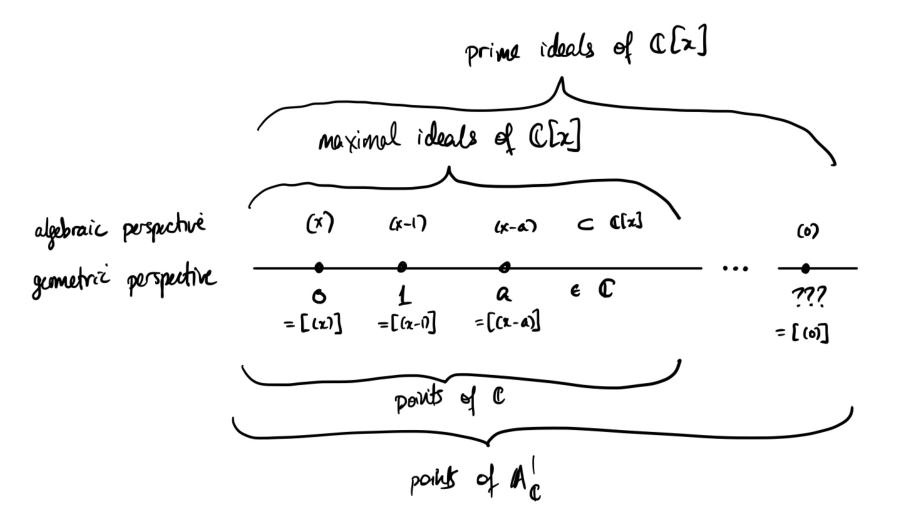
\includegraphics[width=\linewidth,height=\textheight,keepaspectratio]{Figures/complex affine line.png}
    				        \caption{The complex affine line $\A^1_{\bbC}$ (\cite{risingsea}, figure 3.1)}
    				        \label{fig: complex_affine_line}
    				    \end{figure}
    				This result generalises in an obvious manner to algebraically closed fields other than $\bbC$; so for instance, studying schemes over the field $\overline{\Q}$ of algebraic numbers might help one understand more about polynomials with rational coefficients.
    				\item \textbf{(The affine line over a separably closed but not algebraically closed field):} Let $k$ be a field that is separably closed but not algebraically closed (we can take $k = \F_p(t)^{\sep}$, for example). Then, the set of non-zero prime ideals of $\A^1_k$ need not be in bijection with $k$ itself.
    				\item \textbf{(Spectrum of the integers):} The prime ideals of $\Z$ are either generated by prime numbers themselves, or the zero ideal $(0)$. Thus, the set $\Spec \Z$ is in bijection with the \textit{union} of the set of all prime numbers and the set $\{(0)\}$. 
                \end{enumerate}
            \end{example}
        
        \subsubsection{The Zariski topology as a point-set topology} \index{Topology!Zariski}
            \begin{definition}[Zariski-closed subsets] \label{def: zariski_closed}
                Let $R$ be a commutative ring and let $\calF$ be an arbitrary subset of $R$. Then, let us declare that sets of the following form are closed in the to-be Zariski topology:
                    $$V(\calF) := \left\{\p \in \Spec R \mid \p \supset \calF \right\}$$
                When it might be possible to confuse Zariski-closed subsets of different ring spectra, we will write $V_R(\calF)$ instead of simply $V(\calF)$.
            \end{definition}
            \begin{remark}
                Of course, sets of the form $\Spec R \setminus V(\calF)$ are Zariski-open (that is, if we are assuming that the \href{https://ncatlab.org/nlab/show/excluded+middle}{\underline{the Law of Excluded Middle}} holds).
            \end{remark}
            
            \begin{proposition}[Well-definiteness of the Zariski topology] \label{prop: zariski_closed_well_definiteness}
                Let $R$ be an arbitrary commutative ring and assume the Law of Excluded Middle. Then, Zariski-closed subsets as defined in \ref{def: zariski_closed} actually define a topology on $\Spec R$, which of course, is called the Zariski topology.
            \end{proposition}
                \begin{proof}
                    For each subset $\calF$ of $R$, let us write $I(\calF)$ for the $R$-ideal generated by $\calF$. Let us now verify the axioms defining topologies on sets one-by-one.
                        \begin{enumerate}
                            \item \textbf{(The empty set and the whole set are closed):} The empty set is just $V(R)$ and that $\Spec R$ is just $V\left((0)\right)$, which are, by definition, closed in the Zariski topology. Thus, both the empty set and the whole space are Zariski-closed.
                            \item \textbf{(Finite unions of closed sets are closed):} Let $\{V(\calF_{\alpha})\}_{\alpha \in A}$ be a \textit{finite} set of Zariski-closed subsets of $\Spec R$ and consider the following chain of logical \textit{implications} (wherein $\p$ is a prime ideal of $R$, even though this fact can be inferred from the statements themselves):
                                $$
                                    \begin{aligned}
                                        & \p \in \bigcup_{\alpha \in A} V(\calF_{\alpha})
                                        \\
                                        \iff & \exists \alpha \in A: \p \in V(\calF_{\alpha})
                                        \\
                                        \iff & \exists \alpha \in A: \p \supset \calF_{\alpha}
                                        \\
                                        \iff & \bigvee_{\alpha \in A} (\p \supset \calF_{\alpha})
                                        \\
                                        \implies & \forall \left(f_{\alpha}\right)_{\alpha \in A} \in \prod_{\alpha \in A} \calF_{\alpha}: \prod_{\alpha \in A} f_{\alpha} \in \p
                                        \\
                                        \iff & \bigwedge_{\left(f_{\alpha}\right)_{\alpha \in A} \in \prod_{\alpha \in A} \calF_{\alpha}} \left(\prod_{\alpha \in A} f_{\alpha} \in \p\right)
                                        \\
                                        \iff & \p \supset \left\{\prod_{\alpha \in A} f_{\alpha} \: \bigg| \: \forall \alpha \in A: f_{\alpha} \in \calF_{\alpha} \right\}
                                        \\
                                        \iff & \p \in V\left(\left\{\prod_{\alpha \in A} f_{\alpha} \: \bigg| \: \forall \alpha \in A: f_{\alpha} \in \calF_{\alpha} \right\}\right)
                                    \end{aligned}
                                $$
                            wherein the fourth line, in particular, holds due to the fact that ideals, by definition, are closed under scalar multiplication by elements of their ambient rings. Now, to upgrade the fourth line to an equivalence, we can show that:
                                $$\bigwedge_{\left(f_{\alpha}\right)_{\alpha \in A} \in \prod_{\alpha \in A} \calF_{\alpha}} \left(\prod_{\alpha \in A} f_{\alpha} \in \p\right) \implies \bigvee_{\alpha \in A} (\p \supset \calF_{\alpha})$$
                            or, as we have assumed that the Law of Excluded Middle holds, we have the following:
                                $$
                                    \begin{aligned}
                                        & \left(\bigwedge_{\left(f_{\alpha}\right)_{\alpha \in A} \in \prod_{\alpha \in A} \calF_{\alpha}} \left(\prod_{\alpha \in A} f_{\alpha} \in \p\right) \implies \bigvee_{\alpha \in A} (\p \supset \calF_{\alpha})\right)
                                        \\
                                        \vdash & \left(\neg \bigwedge_{\left(f_{\alpha}\right)_{\alpha \in A} \in \prod_{\alpha \in A} \calF_{\alpha}} \left(\prod_{\alpha \in A} f_{\alpha} \in \p\right) \implies  \neg \bigvee_{\alpha \in A} (\p \supset \calF_{\alpha})\right)
                                    \end{aligned}
                                $$
                            meaning that we can prove the contraposition instead. To that end, consider the following:
                                $$
                                    \begin{aligned}
                                        & \neg \bigwedge_{\left(f_{\alpha}\right)_{\alpha \in A} \in \prod_{\alpha \in A} \calF_{\alpha}} \left(\p \ni \prod_{\alpha \in A} f_{\alpha}\right)
                                        \\
                                        \implies & \bigvee_{\left(f_{\alpha}\right)_{\alpha \in A} \in \prod_{\alpha \in A} \calF_{\alpha}} \neg \left(\p \ni \prod_{\alpha \in A} f_{\alpha}\right)
                                        \\
                                        \implies & \bigwedge_{\alpha \in A} \left(\bigvee_{f_{\alpha} \in \calF_{\alpha}} \neg(\p \ni f_{\alpha})\right)
                                        \\
                                        \implies & \bigwedge_{\alpha \in A} \left(\neg \bigwedge_{f_{\alpha} \in \calF_{\alpha}} (\p \ni f_{\alpha})\right)
                                        \\
                                        \implies & \bigwedge_{\alpha \in A} \neg (\p \supset \calF_{\alpha})
                                        \\
                                        \implies & \neg \bigvee_{\alpha \in A} (\p \supset \calF_{\alpha})
                                    \end{aligned}
                                $$
                            Thus, we have managed to show that:
                                $$\neg \bigwedge_{\left(f_{\alpha}\right)_{\alpha \in A} \in \prod_{\alpha \in A} \calF_{\alpha}} \left(\prod_{\alpha \in A} f_{\alpha} \in \p\right) \implies  \neg \bigvee_{\alpha \in A} (\p \supset \calF_{\alpha})$$
                            and therefore:
                                $$\p \in \bigcup_{\alpha \in A} V(\calF_{\alpha}) \iff \p \in V\left(\left\{\prod_{\alpha \in A} f_{\alpha} \: \bigg| \: \forall \alpha \in A: f_{\alpha} \in \calF_{\alpha} \right\}\right)$$
                            Because $\p$ was chosen arbitrarily, this implies that:
                                $$\bigcup_{\alpha \in A} V(\calF_{\alpha}) = V\left(\left\{\prod_{\alpha \in A} f_{\alpha} \: \bigg| \: \forall \alpha \in A: f_{\alpha} \in \calF_{\alpha} \right\}\right)$$
                            Hence, the \textit{finite} union $\bigcup_{\alpha \in A} V(\calF_{\alpha})$ is Zariski-closed by definition, and consequently, all finite unions of Zariski-closed sets are closed in the Zariski topology themselves (since $\{\calF_{\alpha}\}_{\alpha \in A}$ is an arbitrary fintie set of subsets of $R$). Note that the finiteness assumption on the index set $A$ is crucial, as without it, one would not be able to properly make sense of the product $\prod_{\alpha \in A} f_{\alpha}$.
                            \item \textbf{(Intersections of closed sets are closed):} Let $\{V(\calF_{\alpha})\}_{\alpha \in A}$ be an \textit{arbitrary} set of Zariski-closed subsets of $\Spec R$ and consider the following chain of logical equivalences (wherein $\p$ is a prime ideal of $R$, and again, this fact can be deduced from the statements themselves):
                                $$
                                    \begin{aligned}
                                        & \p \in \bigcap_{\alpha \in A} V(\calF_{\alpha})
                                        \\
                                        \iff & \forall \alpha \in A: \p \in V(\calF_{\alpha})
                                        \\
                                        \iff & \forall \alpha \in A: \p \supset \calF_{\alpha}
                                        \\
                                        \iff & \p \supset I\left(\bigcup_{\alpha \in A} \calF_{\alpha}\right)
                                        \\
                                        \iff & \p \in V\left(I\left(\bigcup_{\alpha \in A} \calF_{\alpha}\right)\right)
                                    \end{aligned}
                                $$
                            It tells us that \textit{any} prime ideal $\p$ is in an intersection of Zariski-closed subsets of $\Spec R$ defined by subsets $\calF_{\alpha}$ of $R$ if and only if it is in the Zariski-closed subset of $\Spec R$ defined by the ideal generated by the union of the sets $\calF_{\alpha}$, or in other words, that:
                                $$\bigcap_{\alpha \in A} V(\calF_{\alpha}) = V\left(I\left(\bigcup_{\alpha \in A} \calF_{\alpha}\right)\right)$$
                            In turn, this implies that the intersection of the Zariski-closed sets $V(\calF_{\alpha})$ is itself closed in the Zariski topology, and since the index set $A$ is was chosen arbitrarily, this means that arbitrary intersections of Zariski-closed sets are themselves Zariski-closed.
                        \end{enumerate}
                    Thus, with closed sets as in definition \ref{def: zariski_closed}, the Zariski topology on prime spectra of commutative rings is well-defined.
                \end{proof}
            \begin{corollary}[Quotients are closed] \label{coro: quotients_are_closed}
                Let $R$ be a commutative ring and let $I$ be an $R$-ideal. Then, $\Spec R/I$ is homeomorphic to a Zariski-closed subset of $\Spec R$. 
            \end{corollary}
                \begin{proof}
                    This comes from a straightforward application of the third isomorphism theorem for modules.
                \end{proof}
                
            \begin{definition}[A different approach: Zariski-open sets] \label{def: zariski_open}
                Let $R$ be a commutative ring. Then, let us declare that subsets of $\Spec R$ of the following form are open in the to-be Zariski topology:
                    $$D(f) := \{\p \in \Spec R \mid \p \not \ni f\}$$
                Whenever referring to more than one ring spectra, it might be beneficial to specifically write $D_R(f)$ instead of $D(f)$.
            \end{definition}
            \begin{remark} \label{remark: basic_opens_complements}
                For any commutative ring $R$, one can show through the following logical equivalences that:
                    $$D(f) = \Spec R \setminus V\left((f)\right)$$
                wherein $\p$ is an arbitrary prime ideal of $R$:
                    $$
                        \begin{aligned}
                            & \p \in D(f)
                            \\
                            \iff & \p \in \{\q \in \Spec R \mid \q \not \ni f\}
                            \\
                            \iff & \neg(\p \ni f)
                            \\
                            \iff & \neg(\p \supset (f))
                            \\
                            \iff & \p \in \Spec R \setminus \{\q \in \Spec R \mid \q \supset (f)\}
                            \\
                            \iff & \p \in \Spec R \setminus V\left((f)\right)
                        \end{aligned}
                    $$
            \end{remark}
            
            \begin{proposition}[Well-definiteness of the Zariski topology] \label{prop: zariski_open_well_definiteness}
                Let $R$ be an arbitrary commutative ring and assume the Law of Excluded Middle. Then, Zariski-open subsets as defined in \ref{def: zariski_open} actually define a topology on $\Spec R$, which of course, is called the Zariski topology.
            \end{proposition}
                \begin{proof}
                    Let us verify the axioms defining topologies on sets one-by-one.
                        \begin{enumerate}
                            \item \textbf{(The empty set and the whole set are open):} Consider the set $D(1)$, which by definition, is given by:
                                $$D(1) := \{\p \in \Spec R \mid \p \not \ni 1\}$$
                            Because prime ideals are defined to be proper, and because proper ideals are never (multiplicatively) unital, one gets that:
                                $$D(1) = \Spec R$$
                            In other words, the whole of $\Spec R$ is open by definition. Now, consider the following:
                                $$D(0) := \{\p \in \Spec R \mid \p \not \ni 0\} = \varnothing$$
                            which holds because ideals are submodules of their ambient rings, and modules over rings must contain $0$ (as an additive identity) by definition. Thus, the empty set is also Zariski-open by definition. 
                            \item \textbf{(Unions of open sets are open):} Let $\{f_{\alpha}\}_{\alpha \in A}$ be an \textit{arbitrary} set of elements of $R$ and let us apply remark \ref{remark: basic_opens_complements} to get the following chain of logical equivalences regarding the union of the sets $D(f_{\alpha})$, wherein $\p$ is an \textit{arbitrary} prime ideal of $R$:
                                $$
                                    \begin{aligned}
                                        & \p \in \bigcup_{\alpha \in A} D(f_{\alpha})
                                        \\
                                        \iff & \bigvee_{\alpha \in A} \left(\p \in D(f_{\alpha})\right)
                                        \\
                                        \iff & \bigvee_{\alpha \in A} \neg \left(\p \in V\left((f_{\alpha})\right)\right)
                                        \\
                                        \iff & \neg \bigwedge_{\alpha \in A} \left(\p \in V\left((f_{\alpha})\right)\right)
                                        \\
                                        \iff & \p \in \Spec R \setminus \bigcap_{\alpha \in A} V\left((f_{\alpha})\right)
                                    \end{aligned}
                                $$
                            This shows that:
                                $$\bigcup_{\alpha \in A} D(f_{\alpha}) = \Spec R \setminus \bigcap_{\alpha \in A} V\left((f_{\alpha})\right)$$
                            In proposition \ref{prop: zariski_closed_well_definiteness}, we have already shown using only definition \ref{def: zariski_closed} that arbitrary intersections of Zariski-closed sets are Zariski-closed themselves; in particular, this means that $\bigcap_{\alpha \in A} V\left((f_{\alpha})\right)$ is Zariski-closed. Then, by using the Law of Excluded Middle, one can see that the complement $\Spec R \setminus \bigcap_{\alpha \in A} V\left((f_{\alpha})\right)$ is necessarily Zariski-open. Thus, arbitrary unions of Zariski-open sets are Zariski-open themselves.
                            \item \textbf{(Finite intersections of open sets are open):} Let $\{f_{\alpha}\}_{\alpha \in A}$ be an \textit{finite} set of elements of $R$ and consider the following chain of logical equivalences regarding the union of the sets $D(f_{\alpha})$, wherein $\p$ is a prime ideal of $R$:
                                $$
                                    \begin{aligned}
                                        & \neg \left(\p \in \bigcap_{\alpha \in A} D(f_{\alpha})\right)
                                        \\
                                        \iff & \neg \bigwedge_{\alpha \in A} \left(\p \in D(f_{\alpha})\right)
                                        \\
                                        \iff & \bigvee_{\alpha \in A} \neg \left(\p \in D(f_{\alpha})\right)
                                        \\
                                        \iff & \bigvee_{\alpha \in A} \left(\p \in \Spec R \setminus D(f_{\alpha})\right)
                                        \\
                                        \iff & \bigvee_{\alpha \in A} \left(\p \in V\left((f_{\alpha})\right)\right)
                                        \\
                                        \iff & \p \in \bigcup_{\alpha \in A} V\left((f_{\alpha})\right)
                                    \end{aligned}
                                $$
                            (let us note that the fifth line holds thanks to remark \ref{remark: basic_opens_complements}). Now, the contraposition of the equivalence:
                                $$\neg \left(\p \in \bigcap_{\alpha \in A} D(f_{\alpha})\right) \iff \p \in \bigcup_{\alpha \in A} V\left((f_{\alpha})\right)$$
                            is:
                                $$\neg \neg \left(\p \in \bigcap_{\alpha \in A} D(f_{\alpha})\right) \iff \neg \left(\p \in \bigcup_{\alpha \in A} V\left((f_{\alpha})\right) \right)$$
                            From this, one gets the following proof:
                                $$
                                    \begin{aligned}
                                        & \neg \neg \left(\p \in \bigcap_{\alpha \in A} D(f_{\alpha})\right) \iff \neg \left(\p \in \bigcup_{\alpha \in A} V\left((f_{\alpha})\right) \right)
                                        \\
                                        \vdash & \left(\p \in \bigcap_{\alpha \in A} D(f_{\alpha})\right) \iff \left(\p \in \Spec R \setminus \bigcup_{\alpha \in A} V\left((f_{\alpha})\right) \right) 
                                        \\
                                        \vdash & \left(\bigcap_{\alpha \in A} D(f_{\alpha}) = \Spec R \setminus \bigcup_{\alpha \in A} V\left((f_{\alpha})\right)\right)
                                    \end{aligned}
                                $$
                            Lastly, let us recall that by \ref{prop: zariski_closed_well_definiteness}, the \textit{finite} union $\bigcup_{\alpha \in A} V\left((f_{\alpha})\right)$ of Zariski-closed sets is Zariski-closed itself, meaning that by the Law of Excluded Middle, the complement $\Spec R \setminus \bigcup_{\alpha \in A} V\left((f_{\alpha})\right)$ must be Zariski-open. Thus, the union $\bigcap_{\alpha \in A} D(f_{\alpha})$ is Zariski-open. Note that the finiteness assumption on the index set $A$ is crucial, as otherwise, the union $\bigcup_{\alpha \in A} V\left((f_{\alpha})\right)$ might not be Zariski-closed.
                        \end{enumerate}
                    Thus, with open sets as in definition \ref{def: zariski_open}, the Zariski topology on prime spectra of commutative rings is well-defined.
                \end{proof}
            
            \begin{proposition}[Unifying the two definitions] \label{prop: zariski_topology_equivalence}
                By asuming the Law of Excluded Middle, one gets the same topology on spectra of commutative rings via the approaches presented in definitions \ref{def: zariski_closed} and \ref{def: zariski_open}.
            \end{proposition}
                \begin{proof}
                    Let $R$ be a commutative ring. It is sufficient to show that for each element $f \in R$, the complement $\Spec R \setminus D(f)$ is closed in the sense of definition \ref{def: zariski_closed}, or equivalently, for each subset $\calF \subset R$, the complement $\Spec R \setminus V(\calF)$ is open in the sense of definition \ref{def: zariski_open}. We will be attempting the second approach. To that end, let us directly the following chain of logical equivalences:
                        $$
                            \begin{aligned}
                                & \p \in \bigcup_{\alpha \in A} D(f_{\alpha})
                                \\
                                \iff & \exists \alpha \in A: \p \in D(f_{\alpha})
                                \\
                                \iff & \exists \alpha \in A: \p \in \{\q \in \Spec R \mid \q \not \ni f_{\alpha}\}
                                \\
                                \iff & \exists \alpha \in A: \p \not \ni f_{\alpha}
                                \\
                                \iff & \bigvee_{\alpha \in A} \neg\left(\p \ni f_{\alpha}\right)
                                \\
                                \iff & \neg \bigwedge_{\alpha \in A} (\p \ni f_{\alpha}) 
                                \\
                                \iff & \neg \left(\p \supset \bigcup_{\alpha \in A} \{f_{\alpha}\}\right)
                                \\
                                \iff & \neg \left(\p \supset \{f_{\alpha}\}_{\alpha \in A}\right)
                                \\
                                \iff & \p \in \Spec R \setminus \left\{\q \in \Spec R \mid \q \supset \{f_{\alpha}\}_{\alpha \in A}\right\}
                                \\
                                \iff & \p \in \Spec R \setminus V\left(\{f_{\alpha}\}_{\alpha \in A}\right)
                            \end{aligned}
                        $$
                    Thus:
                        $$\bigcup_{\alpha \in A} D(f_{\alpha}) = \Spec R \setminus V\left(\{f_{\alpha}\}_{\alpha \in A}\right)$$
                    i.e. the complement of the Zariski-closed set $V\left(\{f_{\alpha}\}_{\alpha \in A}\right)$ inside $\Spec R$ is a union of Zariski-open sets $D(f_{\alpha})$, which we know from proposition \ref{prop: zariski_open_well_definiteness} to be Zariski-open itself. As stated, this implies that definitions \ref{def: zariski_closed} and \ref{def: zariski_open} give us the same Zariski topology on prime spectra of commutative rings.
                \end{proof}
            \begin{corollary} \label{coro: zariski_basis}
                Let $R$ be a commutative ring and let $f$ denote elements of $R$. Then, the distinguished Zariski-open sets $D(f)$ form a base of the Zariski topology on $\Spec R$.
            \end{corollary}
                \begin{proof}
                    This is a direct consequence of the fact that complements of Zariski-closed sets are unions of Zariski-open sets of the form $D(f)$.
                \end{proof}
            
            We have managed to show that on each ring spectrum, there is a canonical topology, namely the Zariski topology. A naturaly follow-up question is thus: can we upgrade $\Spec$ to a functor whose domain is $\Top$ instead of $\Sets$ ? Luckily, the answer is yes, although we will need to do some work to show that this is the case. 
            \begin{proposition}[Continuous functions between spectra] \label{prop: continuous_functions_between_spectra}
                By equipping prime spectra of commutative rings with the Zariski topology (in either the sense of definition \ref{def: zariski_closed} or \ref{def: zariski_open}), one naturally gets a functor:
                    $$\Spec: \Cring^{\op} \to \Top$$
                assigning to commutative rings their respective Zariski topological spaces.
            \end{proposition}
                \begin{proof}
                    It will suffice to show that given any ring homomorphism $f: A \to B$, the induced map $\Spec f: \Spec B \to \Spec A$ is continuous, which we can do by showing that preimages of Zariski-open subsets of $\Spec A$ under $\Spec f$ are closed in $\Spec B$; in fact, we can restrict our attention to \textit{basic} open subsets of $\Spec A$ (i.e. subsets of the form $D_A(a)$, for some $a \in A$), as they form a basis for the Zariski topology on $\Spec A$. Let $D_A(a)$ be such a basic open set. It preimage under $\Spec f$ is thus the following subset of $\Spec B$:
                        $$(\Spec f)^{-1}\left(D_A(a)\right) = \{\q \in \Spec B \mid (\Spec f)(\q) \in D_A(a)\}$$
                    Writing out the definition of $D_A(a)$ (cf. definition \ref{def: zariski_open}) then gives the following chain of logical equivalences:
                        $$
                            \begin{aligned}
                                & \q \in (\Spec f)^{-1}\left(D_A(a)\right)
                                \\
                                \iff & (\Spec f)(\q) \in D_A(a)
                                \\
                                \iff & f^{-1}(\q) \in D_A(a)
                                \\
                                \iff & \neg(f^{-1}(\q) \ni a)
                                \\
                                \iff & \neg(\q \ni f(a))
                                \\
                                \iff & \q \in D_B(f(a))
                            \end{aligned}
                        $$
                    which proves that:
                        $$(\Spec f)^{-1}\left(D_A(a)\right) = D_B(f(a))$$
                    and because $D_B(f(a))$ is open by definition, so is the preimage $(\Spec f)^{-1}(D_A(a))$. As stated at the beginning, this implies that $\Spec f$ is a continuous function, and thus there exists a functor:
                        $$\Spec: \Cring^{\op} \to \Top$$
                    assigning commutative rings and homomorphisms between them to ring spectra equipped with the Zariski topology and continuous maps in between.
                \end{proof}
                
            \begin{example}[Topologically interesting ring spectra]
                \noindent
                \begin{enumerate}
                    \item \textbf{(The complex affine plane and complex affine $n$-spaces):}
                        \begin{figure}[H]
                            \centering
                            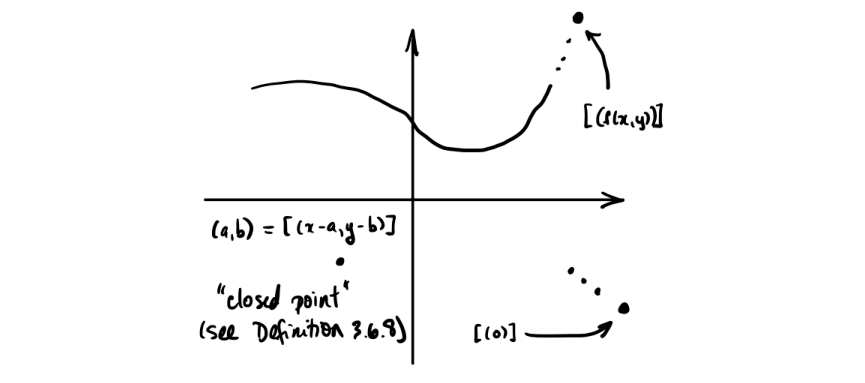
\includegraphics[width=\linewidth,height=\textheight,keepaspectratio]{Figures/complex affine plane.png}
                            \caption{The complex affine plane $\A^2_{\bbC}$ (\cite{risingsea}, figure 3.3)}
                            \label{fig: complex_affine_plane}
                        \end{figure}
                    \item \textbf{(Revisiting $\Spec \Z$):}
                        \begin{figure}[H]
                            \centering
                            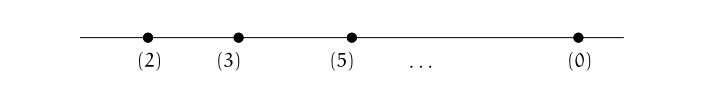
\includegraphics[width=\linewidth,height=\textheight,keepaspectratio]{Figures/Spec Z.png}
                            \caption{$\Spec \Z$ (\cite{risingsea}, figure 3.2)}
                            \label{fig: Spec_Z}
                        \end{figure}
                    \item \textbf{(A conic):}
                        \begin{figure}[H]
                            \centering
                            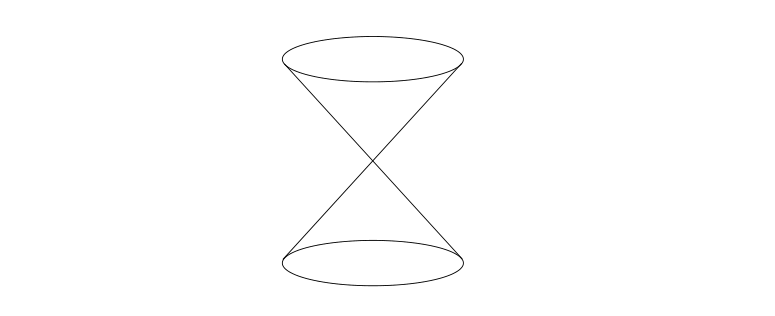
\includegraphics[width=\linewidth,height=\textheight,keepaspectratio]{Figures/conic.png}
                            \caption{A conic which is Zariski-closed inside $\A^3_{\bbC}$ (\cite{risingsea}, figure 3.4)}
                            \label{fig: conic}
                        \end{figure}
                \end{enumerate}
            \end{example}
            
            \begin{remark}[Comparing $\Spec$ and $\Spm$]
                Historically (and only because mathematicians were more interested in complex algebraic geometry back in the days), it was not the set of prime ideals of a commutative ring that was considered, but rather, the set of \textit{maximal} ideals. This was not out of \textit{na\"ivet\'e}, though. Maximal ideals enjoy being closed points in prime spectra of commutative rings (one can prove this by first looking at varieties $V(\m)$ associated to maximal ideals $\m$ of some commutative ring $R$, and then applying the definition of the (underlying set of) these varieties as spaces whose points are prime ideals containing $\m$, and then lastly, applying the usual definition of topological closures; as a corollary, one gets that prime ideals that are not maximal get sent by $\Spec$ to non-closed points in $\Spec R$), and so doing geometry with them is a lot more intuitive (albeit more restrictive as well) then doing so with all prime ideals. For instance, the underlying set of $\Spm \bbC[x]$ is precisely $\bbC$, whereas that of $\Spec \bbC[x]$ can be thought of as $\bbC \cup \{\infty\}$, i.e. as the Riemann sphere; in particular, the zero ideal $(0)$ corresponds to the point \say{at infinity}, which we denote by $\infty$. 
            \end{remark}
            
            \begin{example}[Non-isomorphic rings with homeomorphic spectra] \label{example: nonisomorphic_rings_with_the_same_spectra}
                The following examples are of non-isomorphic rings with homeomorphic prime spectra; through them, we are able to show that the functor $\Spec: \Cring^{\op} \to \Top$ is not an equivalence of categories (nor even a fully faithful inclusion). 
                \begin{enumerate}
                    \item \textbf{(Fields):} The prime spectra of any field is just the one-point space, but clearly, not all fields are isomorphic.
                    \item \textbf{(Discrete valuation rings):} The spectrum of any \href{https://en.wikipedia.org/wiki/Discrete_valuation_ring}{\underline{discrete valuation ring}} is homeomorphic to the \href{https://ncatlab.org/nlab/show/Sierpinski+space}{\underline{Sierpi\'nski space}} (to see why this is the case, firstly check that discrete valuation rings only have two prime ideals, one being the zero ideal and one being the unique maximal ideal, and that the latter is a closed point in the spectrum whereas the former is generic), but of course, not all discrete valuation rings are isomorphic to one another.
                \end{enumerate}
            \end{example}
        
        \subsubsection{Affine schemes}
            Next, we will be discussing the idea of so-call \textbf{structure sheaves}, but in order to make sense of these entities, we will need to know what $\C$-valued sheaves are for categories $\C$ more general than $\Sets$:
            \begin{definition}[$\C$-valued sheaves] \label{def: C_valued_sheaves}
                \noindent
                \begin{enumerate}
                    \item \textbf{($\C$-valued sheaves):} Let $(\S, J)$ be a site\footnote{... which is not necessarily small, as cases such as $\S \cong \Top$ and $\S \cong \Mfd^{\smooth}_{/\R}$ are interesting in their own rights.} and let $\C$ be a category with \textit{enough small limits} and \textit{enough filtered colimits} (the purpose of the second hypothesis is to ensure that stalks, should they exist, are well-defined); note that $\C$ need not be small. Additionally, fix an \textit{arbitrary} object $x$ of $\S$ along with a covering sieve $\calU_{/x} \in J$ thereon. Also, let $j: \S \to \Psh_{\C}(\S)$ be the Yoneda embedding. Then, a \textbf{$\C$-valued sheaf} on $(\S, J)$ is a functor $\calF: \S^{\op} \to \C$ such that $\calF(x) \cong \calF\left( \underset{u \in \calU_{/x}}{\colim} ju \right)$.
                    \item \textbf{($\C$-topoi):} $\C$-valued sheaves on a given site $(\S, J)$ form a category in the obvious manner. We shall be writing $\Sh_{\C}(\S, J)$ for this category, and such categories will be called \textbf{$\C$-topoi}, even though this is an abuse of terminology.
                \end{enumerate}
            \end{definition}
            \begin{example}[Sheaves of rings]
                The notion of sheaves of rings, which subsumes that of structure sheaves (cf. proposition \ref{prop: structure_sheaf}), follows suite from definition \ref{def: C_valued_sheaves}. Note that such constructions are well-defined, as the category of rings is both complete and cocomplete.
            \end{example}
            
            Having defined sheaves that might take values categories other than $\Sets$, let us now try to define affine schemes as locally ringed spaces whose underlying topological spaces are spectra of commutative rings, and whose structure presheaves have a certain condition imposed upon them, which happens to guarantee that:
                \begin{enumerate}
                    \item these structure presheaves are indeed sheaves (proposition \ref{prop: structure_sheaf}) with local stalks (corollary \ref{coro: structure_sheaf_properties}), and
                    \item they are unique (proposition \ref{prop: structure_sheaf_uniqueness}), which is an important feature, because ringed spaces are uniquely defined by their structure sheaves; this fact will also be used to establish the fully faithfulness of $\Spec$ as a functor from $\Cring^{\op}$ to the category $\Loc\Ringed\Spc$ of locally ringed spaces. 
                \end{enumerate}
            Our efforts will culminate in definition \ref{def: affine_schemes}.
                
            \begin{proposition}[Structure sheaves of affine schemes] \label{prop: structure_sheaf} \index{Structure sheaves}
                Let $k$ be a base commutative ring, and let $\calO_{\Spec R}$ be \textit{a} presheaf of commutative rings on $\Ouv(\Spec R)$ determined by the following rule on objects:
                    $$\calO_{\Spec R}(D_R(f)) \cong R_f$$
                for all element $f \in R$. Any presheaf on $\Ouv(\Spec R)$ that are defined this way is a Zariski sheaf (i.e. a sheaf on the site $\Ouv(\Spec R)$ of Zariski-open subsets of $\Spec R$), and is called \textit{a} \textbf{structure sheaf} on $\Spec R$.
            \end{proposition}
            \begin{corollary}[On the locality of stalks] \label{coro: structure_sheaf_properties}
                Let $R$ be a commutative ring and let $\p$ be an arbitrary prime ideal of $R$. Then one has the following characterisation of the stalk $\calO_{\Spec R, \p}$ at $\p$ of the structure sheaf $\calO_{\Spec R}$:
                    $$\calO_{\Spec R, \p} \cong R_{\p}$$
                This shows that affine schemes are, in fact, \textit{locally} ringed spaces and not just ringed spaces. 
            \end{corollary} 
                \begin{proof}
                    Recall that the stalk $\calF_x$ of a sheaf (of sets) $\calF$ on a topological space $(X, \Ouv(X))$ is given by the filtered colimit indexed by the poset of open neighbourhoods of the chosen point $x \in X$:
                        $$\calF_x \cong \underset{U \in \{V \in \Ouv(X) \mid V \ni x\}}{\colim} \calF(U)$$
                    By adapting this definition to the underlying Zariski-topological spaces of affine schemes, we get that:
                        $$\calO_{\Spec R, \p} \cong \underset{U \in \{V \in \Ouv(\Spec R) \mid V \ni \p\}}{\colim} \calO_{\Spec R}(U)$$
                    with $\Ouv(\Spec R)$ the Zariski topology defined via open sets as in definition \ref{def: zariski_open}. In corollary \ref{coro: zariski_basis}, we have already seen how the distinguished Zariski-open sets defined in definition \ref{def: zariski_open} form a basis for the Zariski topology on commutative ring spectra, and so the above filtered colimit can be rewritten as:
                        $$\calO_{\Spec R, \p} \cong \underset{D_R(f) \in \{V \in \Ouv(\Spec R) \mid V \ni \p\}}{\colim} \calO_{\Spec R}\left(D_R(f)\right)$$
                    and because $D_R(f) = \{\p \in \Spec R \mid \p \not \ni f\}$, one subsequently gets:
                        $$\calO_{\Spec R, \p} \cong \underset{f \in \{g \in R \mid g \not \in \p\}}{\colim} \calO_{\Spec R}\left(D_R(f)\}\right)$$
                    Lastly we have the following isomorphism:
                        $$\calO_{\Spec R, \p} \cong \underset{f \in \{g \in R \mid g \not \in \p\}}{\colim} \calO_{\Spec R}\left(D_R(f)\right) \cong \underset{f \in R \setminus \p}{\colim} R_f \cong R_{\p}$$
                    Thus $\calO_{\Spec R, \p} \cong R_{\p}$ as claimed.
                \end{proof}
                
            \begin{proposition}[Uniqueness of structure sheaves] \label{prop: structure_sheaf_uniqueness}
                Let $R$ be a commutative ring. Then, there is only one unique structure sheaf attached to $\Spec R$. 
            \end{proposition}
                \begin{proof}
                    Suppose to the contrary that there exist two \textit{distinct} Zariski sheaves of $R$-algebras on $R\-\Comm\Alg^{\op}$ $\calF$ and $\calG$ such that:
                        $$\forall f \in R: \calF(\Spec R_f) \cong \calG(\Spec R_f) \cong R_f$$
                    However, the localisation of any commutative at its multiplicative identity is just itself, and so:
                        $$\calF(\Spec R) \cong \calG(\Spec R) \cong R$$
                    for all commutative rings $R$. This means that the functors $\calF$ and $\calG$ are naturally isomorphic, i.e. they can not be distinct. Thus, the structure sheaf attached to a given ring spectrum is unique (up to natural isomorphisms, of course).
                \end{proof}
                
            \begin{example}[Spotting structure sheaves in the wild]
                Let $R$ be a discrete valuation ring that is a \href{https://en.wikipedia.org/wiki/Dedekind_domain}{\underline{Dedekind domain}} (so the only proper ideals of $R$ would be $(0)$ and its unique maximal ideal) with unique maximal ideal $\p$, and recall that its spectrum is (homeomorphic to) the Sierpi\'nski space (see example \ref{example: nonisomorphic_rings_with_the_same_spectra} for more details); in particular, the subset $\{(0)\}$ of $\Spec R = \{(0), \p\}$ is the only non-empty open proper subset. Now, suppose that $\calF$ is a Zariski sheaf on $\Spec R$ given by the following formula:
                    $$
                        \calF(U) \cong 
                        \begin{cases}
                            \text{$R$ if $U = \Spec R$}
                            \\
                            \text{$\Frac R$ if $U = \{(0)\}$}
                        \end{cases}
                    $$
                (note that discrete valuation rings are integral domains, so it makes sense to consider their fields of fractions). The point that is to be made here is that $\calF$ qualifies as a structure sheaf on $\Spec R$. To see why this is the case, note that because $R$ has only two prime ideals, namely $(0)$ and $\p$, 
            \end{example}
            
            \begin{example}[The complex affine line]
                Recall that in example \ref{example: spectra_sets}, we have seen how a point of the complex affine line $\A^1_{\bbC}$ is either the zero ideal, or of the form $(t - a)$ for any complex number $a$; one should keep the following picture in mind:
                    \begin{figure}[H]
				        \centering
				        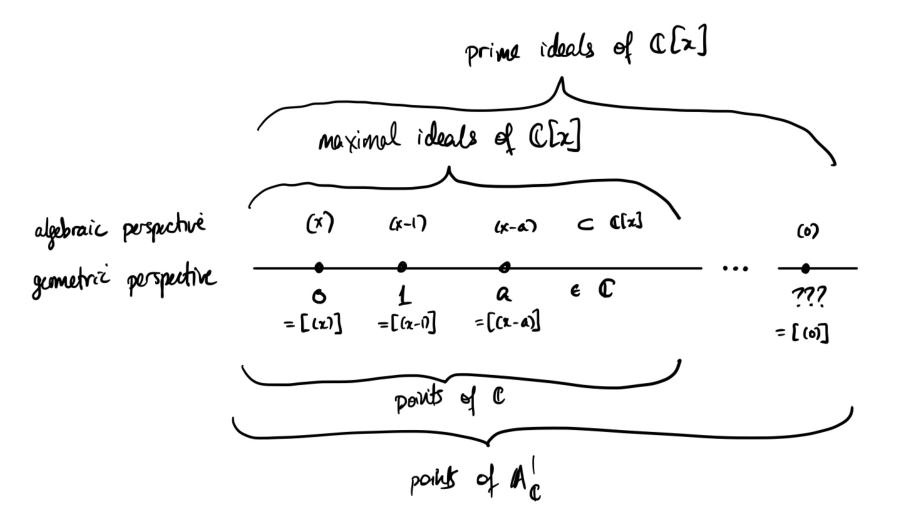
\includegraphics[width=\linewidth,height=\textheight,keepaspectratio]{Figures/complex affine line.png}
				        \caption{The complex affine line $\A^1_{\bbC}$ (\cite{risingsea}, figure 3.1)}
				        \label{fig: complex_affine_line_stalks}
				    \end{figure}
			    \noindent
			    Now, as an affine scheme, $\A^1_{\bbC}$ comes equipped with a structure sheaf $\calO_{\A^1_{\bbC}}$, whose stalks, as shown in corollary \ref{coro: structure_sheaf_properties}, are precisely the localisations of $\bbC[t]$ at its prime ideals. There are thus two cases:
			        \begin{enumerate}
			            \item The stalk at $(0)$ is given by:
			                $$\calO_{\A^1_{\bbC}, (0)} \cong \bbC[t]_{(0)} \cong \bbC(t)$$
		                and thus the residue field is trivially $\bbC(t)$.
			            \item At non-zero primes, the stalks of the structure sheaf $\calO_{\A^1_{\bbC}}$ are given by the following localisations:
			                $$\calO_{\A^1_{\bbC}, (t - a)} \cong \bbC[t]_{(t - a)}$$
		                whose elements we note to be fractions of the form $\frac{f(t)}{g(t)}$ whose denominators do not vanish at $t = a$. Now, recall that the localisation of any commutative ring at a prime ideal is a local ring, and that inside \textit{any} local commutative ring, elements in the complement of the unique maximal ideal are units; in particular, these facts imply that the elements of the complement $\bbC[t]_{(t - a)} \setminus (t - a)\bbC[t]_{(t - a)}$ are all invertible. Consequently, these elements must be fractions $\frac{f(t)}{g(t)}$ whose numerators and denominators both do not vanish at $t = a$. Thus, a reasonable description of the canonical quotient map is the evaluation map:
		                    $$\frac{f(t)}{g(t)} \mapsto \frac{f(a)}{g(a)}$$
	                    whose image is precisely $\bbC$. Therefore, the stalks of $\calO_{\A^1_{\bbC}}$ are all isomorphic to $\bbC$.
			        \end{enumerate}
            \end{example}
        
            \begin{definition}[Affine schemes] \label{def: affine_schemes}
                An \textbf{affine scheme} is a locally ringed space that is isomorphic to one of the form $(|\Spec R|, \calO_{\Spec R})$ for some commutative ring $R$. Morphisms of affine schemes are morphisms of locally ringed spaces, and as such, one has a full subcategory $\Sch^{\aff}$ of affine schemes within the category of locally ringed spaces. 
            \end{definition}
            
            \begin{theorem}[Isbell Duality for locally ringed spaces] \label{theorem: isbell_duality_for_locally_ringed_spaces}
                There is an adjunction as follows:
                    $$
                        \begin{tikzcd}
                        	{\Cring^{\op}} & \Loc\Ringed\Spc
                        	\arrow[""{name=0, anchor=center, inner sep=0}, "\Spec"', bend right, from=1-1, to=1-2]
                        	\arrow[""{name=1, anchor=center, inner sep=0}, "\Gamma"', bend right, from=1-2, to=1-1]
                        	\arrow["\dashv"{anchor=center, rotate=-90}, draw=none, from=1, to=0]
                        \end{tikzcd}
                    $$
            \end{theorem}
            \begin{corollary}
                The adjunction from theorem \ref{theorem: isbell_duality_for_locally_ringed_spaces} restricts down to an adjoint equivalence $\Sch^{\aff} \cong \Cring^{\op}$.
            \end{corollary}

    \subsection{The category of schemes}
        \subsubsection{Schemes}
            \begin{definition}[Schemes] \label{def: schemes}
                A \textbf{scheme} is a locally ringed space $(|X|, \calO_X)$ such that every point $x \in |X|$ as a Zariski-open neighbourhood $U_x \ni x$ that is isomorphic to an affine scheme. Morphisms of schemes are nothing but morphisms of locally ringed spaces, meaning that schemes form a category $\Sch$ which embeds fully faithfully into the category of locally ringed spaces.
            \end{definition}
            
            \begin{proposition}[Open subschemes are open locally ringed subspaces] \label{prop: open_subschemes_are_open_locally_ringed_subspaces}
                Let $X$ be a scheme and let $U \subseteq X$ be an open locally ringed subspace. Then, $U$ will be an open subscheme of $X$. 
            \end{proposition}
                \begin{proof}
                    
                \end{proof}
            \begin{corollary}[Zariski-bases of schemes] \label{coro: zariski_bases_of_schemes}
                
            \end{corollary}
    
        \subsubsection{Properties of schemes and their morphisms}
        
        \subsubsection{Topologies on schemes; descent-theoretic results}
    
    \subsection{Varieties}
        
        \section{Algebraic spaces}
    \subsection{The category of algebraic spaces}
        \subsubsection{Algebraic spaces and their formal properties}
            \begin{convention}[Big sites of schemes] \label{conv: big_sites_of_schemes}
                From this point onwards, we shall be writing $(\Sch_{/S})_{\fppf}$ for the \textit{big} fppf site of a given scheme $S$. In the presence of small sites, which we denote by $(\Sch_{/S})_{\fppf}^{\petit}$, we might write $(\Sch_{/S})_{\fppf}^{\gros}$ for the sake of distinction. Likewise for the \'etale topology.
            \end{convention}
            \begin{convention}[Diagonals] \label{conv: algebraic_spaces_diagonals}
                Let $S$ be a scheme and $F$ be a presheaf of sets on $(\Sch_{/S})_{\fppf}$. We shall be denoting its \textbf{diagonal} by $\Delta_{F/S}: F \to F \x_S F$. This is the morphism of sheaves which is as follows, for all $T \in \Ob((\Sch_{/S})_{\fppf})$:
                    $$\Delta_{F/S}(T): F(T) \to F(T) \x_{S(T)} F(T)$$
                    $$t \mapsto (t, t)$$
            \end{convention}
            
            \begin{lemma}[Permanence of properties of representable morphisms] \label{lemma: permanence_of_properties_of_representable_morphisms}
                Consider sheaves on a site $(\C, J)$, which may or may not be small.
                    \begin{enumerate}
                        \item Representability of morphisms of sheaves is preserved by compositions.
                        \item Representability of morphisms of sheaves is preserved by pullbacks. Also, the diagonal of a representable morphism of sheaves is also representable.
                        \item Let $\varphi: F \to G$ be a representable morphisms of presheaves on $\C$. If $G$ satisfies $J$-descent, then so does $F$.
                    \end{enumerate}
            \end{lemma}
                \begin{proof}
                    \noindent
                    \begin{enumerate}
                        \item 
                        \item 
                        \item 
                    \end{enumerate}
                \end{proof}
            \begin{definition}[Properties of representable morphisms] \label{def: properties_of_representable_morphisms_of_fppf_sheaves}
                Denote by $\calP$ an fppf-local\footnote{Cf. \cite[\href{https://stacks.math.columbia.edu/tag/02KO}{Tag 02KO}]{stacks}.} property of morphisms of schemes that is stable under base-changes\footnote{See \cite[\href{https://stacks.math.columbia.edu/tag/02WE}{Tag 02WE}]{stacks} for a list of such properties.}. Then, one says that a representable morphism of presheaves $\varphi: F \to G$ on $(\Sch_{/S})_{\fppf}$ (for some base scheme $S$) has property $\calP$ if and only if for all schemes $U \in \Ob(\Sch_{/S})$, the canonical projection $\pr_2: F \x_G U \to U$ has property $\calP$ (note that by representability, the pullback $F \x_G U$ is an object of $\Sch_{/S}$).
            \end{definition}
            \begin{proposition}[A representability criterion for diagonals] \label{prop: representability_criterion_for_diagonals}
                Let $S$ be a scheme and let $F$ be a presheaf of sets on $(\Sch_{/S})_{\fppf}$. In addition, suppose that $U, V \in \Ob(\Sch_{/S})$ are two arbitrary $S$-schemes equipped with morphisms $u: U \to F$ and $v: V \to F$, and that the pullback $U_{u, F, v} V$ is representable by some $S$-scheme $T \in \Ob(\Sch_{/S})$. If the canonical morphism $T \to U \x_S V$ has a property $\calP$ that is fppf-local and stable under base-changes, then the diagonal $\Delta_{F/S}: F \to F \x_S F$ must be representable and have property $\calP$.
            \end{proposition}
                \begin{proof}
                    
                \end{proof}
                
            \begin{definition}[Atlases] \label{def: atlases}
                Let $S$ be a scheme and let $F$ be a presheaf of sets on $(\Sch_{/S})_{\fppf}$. An fppf (respectively, \'etale) \textbf{atlas} of $F$ is thus an \'etale surjection $U \to F$ from some scheme $U \in \Ob(\Sch_{/S})$.
            \end{definition}
            \begin{definition}[Algebraic spaces] \label{def: algebraic_spaces}
                An \textbf{algebraic space} over a scheme $S$ is a sheaf of sets on $(\Sch_{/S})_{\fppf}$ with an \'etale atlas and representable diagonal.
            \end{definition}
            \begin{remark}[Algebraic spaces are algebraic stacks]
                Later on, we shall see that algebraic spaces are the same as so-called \textbf{$0$-algebraic stacks}. More on this later, once we have discussed algebraic stacks.
            \end{remark}
            \begin{proposition}[The category of algebraic spaces] \label{prop: the_category_of_algebraic_spaces}
                For any given scheme $S$, there is a category of algebraic spaces over $S$, denoted by $\Alg\Spc_{/S}$, which is a full subcategory of $\Sh(\Sch_{S, \fppf})$. 
            \end{proposition}
                \begin{proof}
                    
                \end{proof}
                
            \begin{proposition}[(Co)limits of algebraic spaces] \label{prop: (co)limits_of_algebraic_spaces}
                For any given scheme $S$, the category $\Alg\Spc_{/S}$ of algebraic spaces over $S$ has the following (co)limits:
                    \begin{enumerate}
                        \item \textbf{(Limits):} terminal objects and finite pullbacks (and hence finite products),
                        \item \textbf{(Colimits):} arbitrary small coproducts.
                    \end{enumerate}
            \end{proposition}
                \begin{proof}
                    \noindent
                    \begin{enumerate}
                        \item \textbf{(Limits):} 
                        \item \textbf{(Colimits):} 
                    \end{enumerate}
                \end{proof}
            \begin{corollary}[Schemes are algebraic spaces] \label{coro: schemes_are_algebraic_spaces}
                For any given scheme $S$, the category $\Sch_{/S}$ of $S$-schemes is a full subcategory of $\Alg\Spc_{/S}$ which is closed under finite pullbacks.
            \end{corollary}
            \begin{remark}[A sheaf-theoretic definition of schemes] \label{remark: sheaf_theoretic_definition_of_schemes}
                In fact, it is easy to see - using the fact that the fppf topology is subcanonical - that \textit{schemes are fppf sheaves $X$ on the category of affine schemes such that their diagonals $\Delta_X$ are representable and such that they admit so-called Zariski atlases, i.e. a jointly surjective family of open immersions $U_i \hookrightarrow X$ from affine schemes $U_i$}. Note that this definition is not circular since one can define schemes either as objects of $\Cring^{\op}$ or as certain kinds of locally ringed spaces, which is a definition that makes use of only the Zariski topology on prime spectra of commutative rings and the notion of structure sheaves.
            \end{remark}
            \begin{definition}[Clopen immersions of ringed spaces] \label{def: clopen_immersions_of_ringed_spaces}
                An immersion of ringed spaces is said to be \textbf{clopen} whenever it is simultaneously closed and open.
            \end{definition}
            \begin{remark}[Clopen immersions of fppf sheaves] \label{remark: clopen_immersions_of_fppf_sheaves}
                Given definition \ref{def: clopen_immersions_of_ringed_spaces}, we can define a \textbf{clopen immersion of sheaves} on $(\Sch_{/S})_{\fppf}$ (with $S$ being some scheme) as a morphism that is representable by clopen immersions of schemes. Note that this is a well-defined notion, as open immersions and closed immersions are stable under base change (since tensor products commute with localisations and quotients) and are fppf-local (cf. \cite[\href{https://stacks.math.columbia.edu/tag/01JY}{Tag 01JY}]{stacks}).
            \end{remark}
            \begin{lemma}[Representability by schemes and algebraic spaces of disjoint summands] \label{lemma: representability_by_schemes_and_algebraic_spaces_of_disjoint_summands}
                Throughout, we work over a base scheme $S$.
                \begin{enumerate}
                    \item Let $F, G$ be sheaves of sets on $(\Sch_{/S})_{\fppf}$. Then, the cannical morphism of sheaves $\iota_1: F \to F \sqcup G$ (or equivalently, $\iota_2: G \to F \sqcup G$) is a clopen immersion.
                    \item Let $X$ be a $S$-scheme (respectively, an algebraic space over $S$) and suppose that there exists a disjoint set $\{F_i\}_{i \in I}$ of sheaves on $(\Sch_{/S})_{\fppf}$ such that $X \cong \coprod_{i \in I} F_i$. Then, each of the disjoint summand $F_i$ will be a clopen subscheme of $X$ (respectively, an algebraic space over $S$ such that the canonical morphism of sheaves $\iota_i: F_i \to X$ is a clopen immersion).
                    \item Let $F$ be a sheaf on $(\Sch_{/S})_{\fppf}$ such that there exists a set $\{F_i\}_{i \in I}$ of open\footnote{In the sense that the inclusions $F_i \hookrightarrow F$ are open immersions. Note that open immersions are fppf-local by virtue of being \'etale, and the reader is invited to check that indeed, open immersions are stable under base change (this is simple consequence of the fact that tensor products and localisations commute).} algebraic subspaces of $F$ such that $\coprod_{i \in I} F_i$ is an algebraic space over $S$ and that the canonically induced morphism of sheaves $\coprod_{i \in I} F_i \to F$ is surjective. In such a situation, $F$ will also be an algebraic space over $S$.
                \end{enumerate}
            \end{lemma}
                \begin{proof}
                    \noindent
                    \begin{enumerate}
                        \item 
                        \item 
                        \item 
                    \end{enumerate}
                \end{proof}
                
            \begin{definition}[\'Etale equivalence relations] \label{def: etale_equivalence_relations}
                Let $S$ be a scheme. An \textbf{\'etale equivalence relation} internal to the category $\Sch_{/S}$ of $S$-schemes (respectively, the category $\Alg\Spc_{/S}$ of algebraic spaces over $S$)\footnote{Note that both categories have all finite pullbacks.} is thus an internal equivalence relation (in the sense of definition \ref{def: equivalence_relations}) whose source and target morphisms are both \'etale.
            \end{definition}
            \begin{lemma}[Base-changing \'etale and flat equivalence relations in schemes] \label{lemma: base_changing_etale_and_flat_equivalence_relations_in_schemes}
                Let $S$ be a scheme, let $U$ be an $S$-scheme, and let $s, t: R \toto U$ be an \'etale equivalence relation on $U$ over $S$.
                    \begin{enumerate}
                        \item \textbf{(\'Etale base-changes):} Suppose that $f: U' \to U$ is an \'etale morphism of $S$-schemes and that $s', t': R' \toto U'$ is the pullback of $s, t: R \toto U$ along $f$. Then, $s', t': R' \toto U'$ will be an \'etale equivalence relation\footnote{Recall that pullbacks of internal equivalence relations are also internal equivalence relations, so $s', t': R' \toto U'$ is \textit{a priori} an equivalence relation on $U'$ over $S$ (cf. \cite[\href{https://stacks.math.columbia.edu/tag/02V8}{Tag 02V8}]{stacks}). Out task here is simply to establish geometric properties of the pullback $s', t': R' \toto U'$, such as whether or not it is \'etale.} on $U'$ over $S$.
                        \item \textbf{(Flat base-changes):} Suppose that the source and target morphisms $s, t: R \toto U$ are surjective, flat, and locally of finite presentation and that $f: U' \to U$ is a morphism of $S$-schemes that is flat and locally of finite presentation; in addition, denote by $s', t': R' \toto U'$ the pullback\footnote{We leave the verification of the fact that being surjective, flat, and locally of finite presentation are properties of morphisms of ($S$-)schemes which are stable under base-changes and are fppf-local up to our readers. } along $f$ of $s, t: R \toto U$. Then, the canonically induced morphism of sheaves $U'R/' \to U/R$ will be an open immersion. 
                    \end{enumerate}
            \end{lemma}
                \begin{proof}
                    \noindent
                    \begin{enumerate}
                        \item \textbf{(\'Etale base-changes):} Consider the following pullback diagrams in $\Sch_{/S}$:
                            $$
                                \begin{tikzcd}
                                	{R'} & {U'} \\
                                	R & U
                                	\arrow["{t'}"', shift right=2, from=1-1, to=1-2]
                                	\arrow["t"', shift right=2, from=2-1, to=2-2]
                                	\arrow["{f_s}"', shift right=2, from=1-1, to=2-1]
                                	\arrow["f", from=1-2, to=2-2]
                                	\arrow["\lrcorner"{anchor=center, pos=0.125}, draw=none, from=1-1, to=2-2]
                                	\arrow["s", shift left=2, from=2-1, to=2-2]
                                	\arrow["{s'}", shift left=2, from=1-1, to=1-2]
                                	\arrow["{f_t}", shift left=2, from=1-1, to=2-1]
                                \end{tikzcd}
                            $$
                        \'Etale morphisms are stable under base-changes so the canonical projections $f_s, f_t: R' \to\to R$ must be \'etale as a consequence of $f: U' \to U$ being \'etale by assumption. Compositions of \'etale morphisms are also \'etale themselves, and since $s, t: R \toto U$ are \'etale morphisms by assumption, the compositions $s \circ f_s$ and $t \circ f_t$ must also be \'etale. As such, the equivalence relation $s', t': R' \toto U'$ is \'etale. 
                        \item \textbf{(Flat base-changes):} By arguing as above and using the fact that surjectivity, flatness, and being locally of finite presentation are properties of morphisms of schemes which are stable under base-changes
                    \end{enumerate}
                \end{proof}
            \begin{proposition}[Base-chaning \'etale and flat equivalence relations in algebraic spaces] \label{prop: base_changing_etale_and_flat_equivalence_relations_in_algebraic_spaces}
                Let $S$ be a scheme, let $\calX$ be an algebraic space over $S$, and let $s, t: R \toto \calX$ be an \'etale equivalence relation on $\calX$ over $S$.
                    \begin{enumerate}
                        \item \textbf{(\'Etale base-changes):} Suppose that $f: \calX' \to \calX$ is an \'etale morphism of algebraic spaces over $\calX$ and that $s', t': R' \toto \calX'$ is the pullback of $s, t: R \toto \calX$ along $f$. Then, $s', t': R' \toto \calX'$ will be an \'etale equivalence relation on $\calX'$ over $S$.
                        \item \textbf{(Flat base-changes):} Suppose that the source and target morphisms $s, t: R \toto \calX$ are surjective, flat, and locally of finite presentation and that $f: \calX' \to \calX$ is a morphism of algebraic spaces over $S$ that is flat and locally of finite presentation; in addition, denote by $s', t': R' \toto \calX'$ the pullback along $f$ of $s, t: R \toto \calX$. Then, the canonically induced morphism of sheaves $\calX'/R' \to \calX/R$ will be an open immersion. 
                    \end{enumerate}
            \end{proposition}
            \begin{definition}[\'Etale presentations of algebraic spaces] \label{def: etale_presentations_of_algebraic_spaces}
                An \textbf{\'etale presentation} of an algebraic space $\calX$ over some scheme $S$, should it exist, is the quotient of an $S$-scheme $U$ by an \'etale equivalence relation $R$ on $U$ such that we have an isomorphism $\calX \cong U/R$ of sheaves on $(\Sch_{/S})_{\fppf}$. Phrased differently, an \'etale presentation of an algebraic space $\calX$ over some scheme $S$ is a coequaliser in $\Sh((\Sch_{/S})_{\fppf})$ of the following form, wherein $U$ and $R$ are as above:
                    $$
                        \begin{tikzcd}
                        	R & U & \calX
                        	\arrow[shift right=2, from=1-1, to=1-2]
                        	\arrow[shift left=2, from=1-1, to=1-2]
                        	\arrow["\coeq", two heads, from=1-2, to=1-3]
                        \end{tikzcd}
                    $$
            \end{definition}
            \begin{proposition}[Existence of \'etale presentation of algebraic spaces] \label{prop: existence_of_etale_presentations_of_algebraic_spaces}
                Let $S$ be a scheme, let $\calX$ be an algebraic space over $S$, and suppose that $\calX$ admits an \'etale atlas $u: U \to \calX$ by an $S$-scheme $U$ (cf. definition \ref{def: algebraic_spaces}). Then, we have the following \'etale presentation for $\calX$, wherein the two arrows $U \x_{u, \calX, u} U \toto U$ come from the canonical morphism $U \x_{u, \calX, u} U \to U \x_S U$:
                    $$
                        \begin{tikzcd}
                        	{U \x_{u, \calX, u} U} & U & \calX
                        	\arrow[shift right=2, from=1-1, to=1-2]
                        	\arrow[shift left=2, from=1-1, to=1-2]
                        	\arrow["{\coeq(u, u)}", two heads, from=1-2, to=1-3]
                        \end{tikzcd}
                    $$ 
            \end{proposition}
                \begin{proof}
                    
                \end{proof}
            \begin{proposition}[Quotients of schemes by \'etale equivalence relations are algebraic spaces] \label{prop: quotients_of_schemes_by_etale_equivalence_relations_are_algebraic_spaces}
                If $U$ is an $S$-scheme and $R$ is an \'etale equivalence relation on $U$, then not only will the sheaf $U/R$ be an algebraic space, but furthermore, the quotient morphism $U \to U/R$ will be \'etale\footnote{Because the quotient morphism $U \to U/R$ is \'etale, the \'etale presentation $R \toto U$ determines an \'etale atlas $U \to U/R$ of the algebraic space $U/R$.} surjection of sheaves on $(\Sch_{/S})_{\fppf}$. 
            \end{proposition}
                \begin{proof}
                    
                \end{proof}
                
            \begin{proposition}[Pushouts of algebraic spaces] \label{prop: puhsouts_of_algebraic_spaces}
                
            \end{proposition}
    
        \subsubsection{Properties of algebraic spaces and their morphisms}
        
        \subsubsection{Topologies on algebraic spaces; descent-theoretic results}
        
        \subsubsection{Criteria for sheaves being algebraic spaces}
    
    \subsection{Algebraic spaces over fields}
        
        \section{Algebraic stacks}
    \subsection{The \texorpdfstring{$2$}{}-category of algebraic stacks}
        \subsubsection{Algebraic stacks and their formal properties}
    
        \subsubsection{Properties of algebraic stacks and their morphisms}
        
        \subsubsection{Topologies on algebraic stacks; descent-theoretic results}
    
    \subsection{Moduli spaces of algebraic stacks}
        \subsubsection{Coarse moduli spaces and the Keel-Mori Theorem}
            In this subsubsection, we attempt to state and prove the Keel-Mori Theorem, which establishes a criterion for certain kinds of algebraic stacks to admit coarse moduli spaces. From there, we will discuss certain applications thereof: in particular, we will be touching on Chow's Lemma for algebraic stacks, as well as a valuative criterion for properness for algebraic stacks.
            
            Before we begin, however, we shall need to actually introduce the notion of a \say{moduli space}, which are of a certain kind of morphism from algebraic stacks to algebraic spaces. The extra conditions are imposed so that they would behave well with respect to various geometric constructions, but essentially, moduli spaces exist to exemplify the idea that algebraic stacks are geometric objects with \say{automorphisms at each point}.
            \begin{definition}[Coarse moduli spaces] \label{def: coarse_moduli_spaces}
                \cite[Section 1, pp. 1]{conrad_keel_mori_theorem_via_stacks} Let $\scrX$ be an algebraic stack over a given scheme $S$ and suppose that $\pi: \scrX \to \calX$ is a morphism to some algebraic space $\calX$ over $S$. We say that $\calX$ is a \textbf{coarse moduli space} for $\scrX$ via $\pi$ (or rather, that the morphism of algebraic stacks $\pi: \scrX \to \calX$ is a coarse moduli space for $\scrX$) if $\pi$ is initial among all morphisms from $\scrX$ to algebraic spaces over $S$ and if for all algebraically closed fields $k$ (i.e. geometric points), the canonically induced function $[\pi(k)]: [\scrX(k)] \to \calX(k)$ is a bijection.  
            \end{definition}
            \begin{remark}[On the (non)representability of coarse moduli spaces] \label{remark: (non)representability_of_coarse_moduli_spaces}
                Clearly, every algebraic space when viewed as a tautological algebraic stack is its own coarse moduli space and conversely, should a Deligne-Mumford stack admit a coarse moduli space then that modui space would be an algebraic space. The converse situation need not be true, stemming from the fact that general algebraic stacks \textit{a priori} admit only smooth atlases. 
            \end{remark}
            \begin{definition}[Fine moduli spaces] \label{def: fine_moduli_spaces}
                A \textbf{fine moduli space} over a scheme $S$ is nothing but a representable presheaf on $\Sch_{/S}$.
            \end{definition}
            \begin{remark}[On the sheafiness of moduli spaces] \label{remark: sheafiness_of_moduli_spaces}
                Many of the common Grothendieck topologies on the category of schemes (e.g. Zariski, \'etale, fppf, fpqc, etc.) are subcanonical and as such fine moduli spaces are automaticallly sheaves with respect to these topologies. 
                
                For coarse moduli spaces, the situation is a bit more subtle. By definition, algebraic spaces satisfy fppf descent and therefore, they must also satisfy \'etale and Zariski descent; a result by Gabber (cf. \cite[\href{https://stacks.math.columbia.edu/tag/0APL}{Tag 0APL}]{stacks}) tells us that algebraic spaces also satisfy fpqc descent, but this is not at all trivial. As such, coarse moduli spaces of Deligne-Mumford stacks (which are algebraic spacess) satisfy Zariski, \'etale, fppf, and fpqc descent. 
            \end{remark}
            \begin{definition}[Stability of coarse moduli spaces] \label{def: stability_of_coarse_moduli_spaces}
                \footnote{Note that this definition also makes sense for fine moduli spaces as fine moduli spaces are coarse moduli spaces by definition (as schemes are instances of algebraic spaces), but because those are nothing but schemes (which form a category with all finite pullbacks, the question of whether or not the formation of a fine moduli space is stable under base-change along representable morphisms is tautological.)}Suppose that $\pi: \scrX \to \calX$ is a coarse moduli space for some algebraic stack $\scrX$ over a given scheme $S$. We say that the formation of this coarse moduli spaces is compatible with flat (respectively, smooth, \'etale, etc.) base-changes if and only if for all flat (respectively, smooth, \'etale, etc.) morphisms $f: \calX' \to \calX$ of algebraic spaces, the canonically induced morphism $\scrX \x^2_{\pi, \calX, f} \calX' \to \calX'$ is also a coarse moduli space.   
            \end{definition}
            \begin{remark}[The importance of flat base-changes] \label{remark: flat_base_changes_of_coarse_moduli_spaces}
                Aside from encompassing the many important cases of base-change, such as smooth and \'etale base-changes, flat morphisms also arise naturally in algebraic geometry: Zariski localisations, for instance, are flat morphisms due to localisations and tensor products commuting. As such, we pay extra attention to whether or not the formation of coarse moduli spaces is preserved by flat base-changes. 
            \end{remark}
            
            \begin{definition}[Well-nigh affine algebraic stacks] \label{def: well_nigh_affine_algebraic_stacks}
                \cite[\href{https://stacks.math.columbia.edu/tag/0DUL}{Tag 0DUL}]{stacks} An algebraic stack $\scrX$ is said to be \textbf{well-nigh affine-schematic}\footnote{... or simply \textbf{well-nigh affine}.} (respecitvely, well-nigh schematic) over a given scheme $S$ if and only if there exists an affine $S$-scheme $U$ along with an atlas $U \to \scrX$ that is flat, finite (respecitvely, quasi-finite), and of finite presentation (respectively, Zariski-locally of finite-presentation) over $S$. 
            \end{definition}
            \begin{remark}
                It is clear from the definition that being well-nigh affine implies being well-nigh schematic.
            \end{remark}
            \begin{remark}[Well-nigh schematicity is fppf local] \label{remark: well_nigh_schematicity_is_fppf_local}
                Flatness, (quasi-)finiteness, and being (Zariski-locally) of finite presentation are all fppf local properties which are fppf-local and stable under base-changes along representable morphisms (cf. \cite[\href{https://stacks.math.columbia.edu/tag/02WE}{Tag 02WE}]{stacks}). Therefore, for an algebraic stack to be well-nigh affine (respectively, well-nigh schematic) is a property that is fppf-local, and hence \'etale and Zariski-local, as well as stable under base-changes along representable morphisms.
                
                Note also that because being well-nigh affine (respectively, well-nigh schematic) is Zariski-local, one can check whether or not an algebraic stack is well-nigh schematic via checking whether or not it is well-nigh affine. The notion of well-nigh schematicity is therefore redundant in practice.
            \end{remark}
            \begin{proposition}[Well-nigh affine algebraic spaces] \label{prop: well_nigh_affine_algebraic_spaces}
                A well-nigh affine algebraic space is nothing but an affine scheme. 
            \end{proposition}
                \begin{proof}
                    
                \end{proof}
            \begin{proposition}[Criteria for well-nigh affineness] \label{prop: well_nigh_affineness_criteria_for_algebraic_stacks}
                \noindent
                \begin{enumerate}
                    \item Let $f: \scrX' \to \scrX$ be an affine morphism of algebraic stacks. Then $\scrX'$ will be well-nigh affine.
                    \item Suppose that $\scrX$ is an algebraic stack over a given scheme $S$. Then, $\scrX$ is well-nigh affine over $S$ if and only if there exists a finite locally free groupoid in $S$-schemes $s, t: R \toto U$ such that $\scrX \cong [U/R]$. 
                \end{enumerate}
            \end{proposition}
                \begin{proof}
                    
                \end{proof}
            \begin{lemma}[Existence of coarse moduli spaces of well-nigh affine algebraic stacks] \label{lemma: existence_of_coarse_moduli_spaces_of_well_nigh_affine_algebraic_stacks}
                Any well-nigh affine algebraic stack $\scrX$ over a given scheme $S$ admits a coarse moduli space $\pi: \scrX \to \calX$ whose formation is stable under flat base-changes. Moreover, the morphism $\pi$ is separated, quasi-compact, and universally homeomorphic over $S$.
            \end{lemma}
                \begin{proof}
                    
                \end{proof}
            \begin{lemma}[A reduction step for the Keel-Mori Theorem] \label{lemma: keel_mori_reduction_step}
                Let $\scrX$ be an algebraic stack Zariski-locally of finite presentation, whose diagonal $\Delta_{\scrX/S}$ is quasi-compact and separated, both over some given scheme $S$. Suppose furthermore that the diagonal $\Delta_{\scrX/S}$ is quasi-finite over $S$. In such a setting, there exists a covering of $\scrX$ by a set $\{\scrX_i\}_{i \in I}$ of open algebraic substacks such that each $\scrX_i$ admits a quasi-finite, flat, and finitely presented scheme atlas $U_i \to \scrX_i$.
            \end{lemma}
                \begin{proof}
                    
                \end{proof}
                
            \begin{definition}[Inertia stacks] \label{def: inertia_stacks}
                Let $f: \scrY \to \scrX$ be a morphism of algebraic stacks over a given scheme $S$. Its associated \textbf{inertia stack} $\Inert(\scrY/\scrX)$ is given by the $2$-pullback of the diagonal $\Delta_{\scrY/\scrX}: \scrY \to \scrY \x_{\scrX} \scrY$ along itself, i.e. it fits into the following $2$-pullback square:
                    $$
                        \begin{tikzcd}
                        	{\Inert(\scrY/\scrX)} & \scrY \\
                        	\scrX & {\scrY \x_{\scrX} \scrY}
                        	\arrow["{\Delta_{\scrY/\scrX}}", from=2-1, to=2-2]
                        	\arrow["{\Delta_{\scrY/\scrX}}", from=1-2, to=2-2]
                        	\arrow[from=1-1, to=2-1]
                        	\arrow[from=1-1, to=1-2]
                        	\arrow["2"{description}, "\lrcorner"{anchor=center, pos=0.125}, draw=none, from=1-1, to=2-2]
                        \end{tikzcd}
                    $$
            \end{definition}
            \begin{proposition}[Properties of inertia stacks] \label{prop: properties_of_inertia_stacks}
                Let $f: \scrY \to \scrX$ be a morphism of algebraic stacks over a given scheme $S$. Then, not only is the inertia stack $\Inert(\scrY/\scrX)$ an algebraic stack over $S$ as well, but also, the canonical projections $\pr_1, \pr_2: \Inert(\scrY/\scrX) \toto \scrY$ are both representable by morphisms locally of finite type between algebraic space over $S$. 
            \end{proposition}
                \begin{proof}
                    
                \end{proof}
            \begin{remark}[Inertia and automorphisms] \label{remark: inertia_and_automorphisms}
                Fix an algebraic stack $\scrX$ over a given base scheme $S$ and consider the evident full $2$-category\footnote{Defined in the manner of definition \ref{def: slice_2_categories}.} $\Alg\Spc_{/\scrX} \overset{2}{\subset} \Alg\Stk_{/\scrX}$ of algebraic spaces over $\scrX$. Observe that this category is $2$-equivalent to the $2$-category 
            \end{remark}
            \begin{proposition}
                Suppose that $\scrX$ is a well-nigh affine algebraic stack and $f: \scrX' \to \scrX$ is an \'etale (respectively, \'etale and separated) morphism of between well-nigh affine algebraic stacks, both over a fixed base scheme $S$. Suppose furthermore that $f$ induces isomorphisms on automorphism groups, and recall that by virtue of being well-nigh affine, the algebraic stack $\scrX$ admit a coarse moduli space $\pi: \scrX \to \calX$ over $S$ whose formation is stable under flat base-changes and such that the morphism $\pi$ is separated, quasi-compact, and universally homeomorphic over $S$.
                
                In such a situation, there exists an \'etale (respectively, \'etale and separated) morphism $g: \calX' \to \calX$ of algebraic spaces over $S$ such that the following diagram is a $2$-pullback square of algebraic stacks over $S$:
                    $$
                        \begin{tikzcd}
                        	{\scrX'} & \scrX \\
                        	{\calX'} & \calX
                        	\arrow["\pi", from=1-2, to=2-2]
                        	\arrow["g", from=2-1, to=2-2]
                        	\arrow[from=1-1, to=2-1]
                        	\arrow["f", from=1-1, to=1-2]
                        	\arrow["\lrcorner"{anchor=center, pos=0.125}, draw=none, from=1-1, to=2-2]
                        \end{tikzcd}
                    $$
            \end{proposition}
                \begin{proof}
                    
                \end{proof}
                
            \begin{theorem}[The Keel-Mori Theorem on the existence of coarse moduli spaces] \label{theorem: keel_mori_theorem_on_the_existence_of_coarse_moduli_spaces}
                
            \end{theorem}
                \begin{proof}
                    
                \end{proof}
        
        \subsubsection{Tame algebraic stacks}
            One of the issues with the notion of (coarse) moduli spaces of algebraic stacks is that it is not very stable. For instance, it is not always the case that the formation of coarse moduli spaces - especially in positive characteristics - commutes with base-changes. As such, it is worthwhile to single out a class of algebraic stacks (so-called \say{tame algebraic stacks}) for which the formation of coarse moduli spaces is actually stable under base-changes; these algebraic stacks also behave well in other ways, but these are rather technical properties, so we thought it best to discuss them later on, once we have had all the definitions in place. 
        
        \begin{appendices}
            \chapter{Fibred categories, descent, and stacks}
                \begin{abstract}
            
                \end{abstract}
                
                \minitoc
                
                \section{Fibred categories}
    \subsection{Generalities on \texorpdfstring{$2$}{}-categories}
        \subsubsection{\textit{Pr\'elude}: Internal categories}
            \begin{definition}[Spans] \label{def: spans} \index{Spans}
                \noindent
                \begin{enumerate}
                    \item \textbf{(Spans):} A \textbf{span} (also known as a \textbf{correspondence}) from an object $x$ to another object $y$ via an object $s$ inside a given category $\C$ is a diagram therein that is of the following form:
                        $$
                            \begin{tikzcd}
                            	s & y \\
                            	x
                            	\arrow["f"', from=1-1, to=2-1]
                            	\arrow["g", from=1-1, to=1-2]
                            \end{tikzcd}
                        $$
                    wherein the tip $s$ is some \textit{choice} of object of $\C$. As any span with either or both arrow therein being an identity is just a normal morphism, the notion of spans can be thought of as a generalisation of morphisms.  
                    \item \textbf{(Categories of spans):} Within a category $\C$ with pullbacks, one can compose, say, a span from $x$ to $y$ via $s$ with another from $y$ to $z$ via $s'$ via taking the pullback of the \say{inner} arrows in the manner depicted by the following diagram:
                        $$
                            \begin{tikzcd}
                            	{s \x_{g, y, f'} s'} & {s'} & z \\
                            	s & y \\
                            	x
                            	\arrow["f"', from=2-1, to=3-1]
                            	\arrow["g"', from=2-1, to=2-2]
                            	\arrow["{f'}", from=1-2, to=2-2]
                            	\arrow["{g'}", from=1-2, to=1-3]
                            	\arrow[from=1-1, to=2-1]
                            	\arrow[from=1-1, to=1-2]
                            	\arrow["\lrcorner"{anchor=center, pos=0.125}, draw=none, from=1-1, to=2-2]
                            \end{tikzcd}
                        $$
                    to obtain a so-called \say{composite} span from $x$ to $z$ via $s \x_{g, y, f'} s'$ (which visually, can be thought of either as the upper \say{roof} or the big \say{roof} covering the two smaller ones - that being the previously specified spans from $x$ to $y$ via $s$ and the span from $y$ to $z$ via $s'$ - in the above diagram); alternatively, one might visualise this composition via the following commutative diagram of spans:
                        $$
                            \begin{tikzcd}
                            	x & y & z
                            	\arrow["{(f,g)}", "\shortmid"{marking}, from=1-1, to=1-2]
                            	\arrow["{(f' g')}", "\shortmid"{marking}, from=1-2, to=1-3]
                            \end{tikzcd}
                        $$
                    With the use of this style of composition, one obtains, for every category $\C$ with pullbacks in tandem with a choice of natural number $n \geq 1$, a (lax) \textbf{$n$-category of spans} $\Span^{\leq n}(\C)$ that is defined via:
                        \begin{enumerate}
                            \item objects being those of $\C$ itself,
                            \item $1$-morphisms being spans between objects, which shall henceforth be known as $1$-spans,
                            \item and for all $2 \leq k \leq n$, $k$-morphisms, which shall henceforth be called $k$-spans, being $k$-cells between $(k-1)$-morphisms; for instance, a $2$-span between two $1$-spans is a commutative diagram of the following form:
                                $$
                                    \begin{tikzcd}
                                        \bullet \arrow[rd] \arrow[rdd, bend right] \arrow[rrd, bend left] &                             &         \\
                                                                                                          & \bullet \arrow[d] \arrow[r] & \bullet \\
                                                                                                          & \bullet                     &        
                                    \end{tikzcd}
                                $$
                        \end{enumerate}
                \end{enumerate}
            \end{definition}
            \begin{convention}[Regarding notations] \label{conv: span_notations}
                Obviously, writing out spans explicitly takes up a lot of effort and frankly, these diagrams can get confusing rather quickly. However, a quick observation tells us that because composites of spans are given by pullbacks, they actually satisfy the universal property of products taken in the arrow category of some given span category. That is to say, given an ambient category $\C$ with all pullbacks and two composable spans:
                    $$
                        \begin{tikzcd}
                        	& \bullet & \bullet \\
                        	\bullet & \bullet \\
                        	\bullet
                        	\arrow["f"', from=2-1, to=3-1]
                        	\arrow["g", from=2-1, to=2-2]
                        	\arrow["{f'}", from=1-2, to=2-2]
                        	\arrow["{g'}", from=1-2, to=1-3]
                        \end{tikzcd}
                    $$
                therein, their composite:
                    $$
                        \begin{tikzcd}
                        	\bullet & \bullet & \bullet \\
                        	\bullet & \bullet \\
                        	\bullet
                        	\arrow["f"', from=2-1, to=3-1]
                        	\arrow["g"', from=2-1, to=2-2]
                        	\arrow["{f'}", from=1-2, to=2-2]
                        	\arrow["{g'}", from=1-2, to=1-3]
                        	\arrow[from=1-1, to=2-1]
                        	\arrow[from=1-1, to=1-2]
                        	\arrow["\lrcorner"{anchor=center, pos=0.125}, draw=none, from=1-1, to=2-2]
                        \end{tikzcd}
                    $$
                is nothing but the product:
                    $$
                        \begin{tikzcd}
                        	{(f, g) \x (f', g')} & {(f', g')} \\
                        	{(f, g)}
                        	\arrow[dashed, from=1-1, to=2-1]
                        	\arrow[dashed, from=1-1, to=1-2]
                        \end{tikzcd}
                    $$
                in $\Mor\left(\Span^{\leq 1}(\C)\right)$ (which will probably be commonly written as $\Span^{\leq 1}(\C)_1$ from now on, so as to make the notion of spans fit snuggly into the language of internal categories, and also to cut back on parentheses) Therefore, our proposition of an alternative notation is as follows: the composition of two spans $(f, g)$ and $(f', g')$ shall instead be denoted by $(f, g) \x (f', g')$.
            \end{convention}
            \begin{convention}[Associators]
                Fix a \textit{weak} $n$-category $\C$, with $n \geq 1$. Now, for all $1 \leq k \leq n$ and all triples of \textit{composable} $(k - 1)$-morphisms $f, g, h$ of $\C$, let us call the $k$-cell:
                    $$(fg)h \to f(gh)$$
                (which we note to be invertible thanks to the weakness assumption on $\C$) a \textbf{$k$-associator}. An associator is called \textbf{trivial} if and only if it is an identity. See \href{https://ncatlab.org/nlab/show/associator}{\underline{here}} for more details. 
            \end{convention}
            \begin{remark}[Associators in span categories]
                Since pullbacks are merely unique up to unique isomorphisms, $k$-associators in the $n$-category $\Span^{\leq n}(\C)$ of spans of a given category $\C$ with pullbacks are generally non-trivial, but they are invertible. This implies that $n$-categories of spans are \textit{weak} $n$-categories, as opposed to simply being lax $n$-categories, but generally they are not strict $n$-categories. 
            \end{remark}
            
            \begin{proposition}[Limits and colimits of spans]
                
            \end{proposition}
        
            \begin{definition}[Internal categories] \label{def: internal_categories}
                Let $\E$ be a category with \textit{enough pullbacks}. A category \textbf{internal} to $\E$ is then a pair $(C_0, C_1)$ of objects of $\E$ defined via the following data:
                    \begin{enumerate}
                        \item \textbf{(Objects and morphisms):} An object of \textbf{objects} $C_0 \in \E$ and an object of \textbf{arrows} $C_1 \in \E$, both are to be viewed as internal analogues of the collections of objects and arrows in the definition of categories.
                        \item \textbf{(Composition):} 
                            \begin{enumerate}
                                \item \textbf{(Sources and targets):} From the object of arrows $C_1$ to the object of objects $C_0$, there are two morphisms $s, t$ as follows, known as the \textbf{source} and \textbf{target} maps:
                                    $$
                                        \begin{tikzcd}
                                        	{C_1} & {C_0}
                                        	\arrow["s", shift left=2, from=1-1, to=1-2]
                                        	\arrow["t"', shift right=2, from=1-1, to=1-2]
                                        \end{tikzcd}
                                    $$
                                which, respectively, assign to each arrow $f \in C_1$ (which, along with similar instances, shall be viewed as a \href{https://ncatlab.org/nlab/show/generalized+element}{\underline{generalised elements}} for the sake of linguistic convenience) its domain and codomain objects in $C_0$.
                                \item \textbf{(Units):} From the object of objects $C_0$ to the object of arrows $C_1$, there is a distinguished morphism:
                                    $$e: C_0 \to C_1$$
                                called the \textbf{unit map} which assigns to each object $x \in C_0$ (again, viewed as a generalised element) the identity $\id_x: x \to x$ thereon, which we note to be an a generalised element of the object of arrows $C_1$ (hence the codomain of $e$ is $C_1$).
                                \item \textbf{(Composition of arrows):} There is a monoidal composition operation (in the sense of monoidal categories):
                                    $$\mu: C_1 \x_{s, C_0, t} C_1 \to C_1$$
                                satisfying the following conditions specified by commutative diagrams in $\E$:
                                    \begin{enumerate}
                                        \item \textbf{(Identities do not alter domains and codomains):}
                                            $$
                                                \begin{tikzcd}
                                                	{C_0} & {C_1} && {C_0} & {C_1} \\
                                                	& {C_0} &&& {C_0}
                                                	\arrow["e", from=1-1, to=1-2]
                                                	\arrow["{\id_{C_0}}"', from=1-1, to=2-2]
                                                	\arrow["s", from=1-2, to=2-2]
                                                	\arrow["{\id_{C_0}}"', from=1-4, to=2-5]
                                                	\arrow["t", from=1-5, to=2-5]
                                                	\arrow["e", from=1-4, to=1-5]
                                                \end{tikzcd}
                                            $$
                                        \item \textbf{(Sources and targets of compositions):} The source of a composition $g \mu f \in C_1$ should be that of $f$ (the former), wheareas its target should be that of $g$ (the latter): 
                                            $$
                                                \begin{tikzcd}
                                                	& {C_1 \x_{s, C_0, t} C_1} & {C_1} && {C_1 \x_{s, C_0, t} C_1} & {C_1} \\
                                                	{} & {C_1} & {C_0} && {C_1} & {C_0}
                                                	\arrow["s", from=1-3, to=2-3]
                                                	\arrow["s", from=2-2, to=2-3]
                                                	\arrow["{\pr_2}"', from=1-2, to=2-2]
                                                	\arrow["{\pr_1}", from=1-2, to=1-3]
                                                	\arrow["t", from=1-6, to=2-6]
                                                	\arrow["t", from=2-5, to=2-6]
                                                	\arrow["{\pr_1}"', from=1-5, to=2-5]
                                                	\arrow["{\pr_1}", from=1-5, to=1-6]
                                                \end{tikzcd}
                                            $$
                                        \item \textbf{(Associativity):} 
                                            $$
                                                \begin{tikzcd}
                                                	& {C_1 \x_{s, C_0, t} C_1 \x_{s, C_0, t} C_1} & {C_1 \x_{s, C_0, t} C_1} \\
                                                	{} & {C_1 \x_{s, C_0, t} C_1} & {C_1}
                                                	\arrow["\mu", from=1-3, to=2-3]
                                                	\arrow["\mu", from=2-2, to=2-3]
                                                	\arrow["{\id_{C_1} \x_{s, C_0, t} \mu}"', from=1-2, to=2-2]
                                                	\arrow["{\mu \x_{s, C_0, t} \id_{C_1}}", from=1-2, to=1-3]
                                                \end{tikzcd}
                                            $$
                                        \item \textbf{(Left and right-unitarity):} 
                                    \end{enumerate}
                                        $$
                                            \begin{tikzcd}
                                            	{C_0 \x_{C_0} C_1} & {C_1 \x_{s, C_0, t} C_1} & {C_1 \x_{C_0} C_0} \\
                                            	& {C_1}
                                            	\arrow["\mu", from=1-2, to=2-2]
                                            	\arrow["{\pr_2}"', from=1-1, to=2-2]
                                            	\arrow["{\pr_1}", from=1-3, to=2-2]
                                            	\arrow["{\e \x_{C_0} \id_{C_1}}", from=1-1, to=1-2]
                                            	\arrow["{\id_{C_1} \x_{C_0} e}"', from=1-3, to=1-2]
                                            \end{tikzcd}
                                        $$
                                with the latter three specifying the monoidality of the composition operation $\mu$.
                            \end{enumerate}
                    \end{enumerate}
            \end{definition}
            
            \begin{remark}[Internal categories vs. subcategories]
                    
            \end{remark}
            
            \begin{remark}[Another formulation: Internal categories as monads on spans] \label{remark: internal_categories_alt_def}
                Definition \ref{def: internal_categories} gives us a perfectly fine idea of what one might mean by \say{internal categories}. However, it is manifestly rather clunky. Therefore, the author has taken the liberty to provide one alternative formulation of the notion of internal categories.
                
                We refer the reader to definition \ref{def: spans} and the discussion that follows for necessary information on the paradigm of spans; in particular, let us recall that spans are only well-defined inside categories with pullbacks (which is a slightly stronger condition than the assumption in definition \ref{def: internal_categories} that the ambient category as merely \textit{enough} pullbacks). 
                    
                Now, let $\E$ be an ambient category with all pullbacks, and subsequently, let us define a category $C$ internal to $\E$ as being the same as a monad in the weak $2$-category $\Span^{\leq 2}(\E)$ of spans on $\E$. Why would this even resemble a reasonable definition of categories internal to a given category $\E$ ? For starters, recall that a monad is an endomorphism satisfying so-called \say{monoidal multiplication}. Therefore, an internal category $C$ inside a given ambient category $\E$ is first and foremost an endomorphism on a choice of object, and because the weak $2$-category in which we are trying to build monads is one of spans, our endomorphism should be a \say{roof} diagram whose two \say{lower} vertices are the same. By consulting definition \ref{def: internal_categories}, one sees that an obvious choice is the source-target span:
                    $$
                        \begin{tikzcd}
                        	{C_1} & {C_0} \\
                        	{C_0}
                        	\arrow["s"', from=1-1, to=2-1]
                        	\arrow["t", from=1-1, to=1-2]
                        \end{tikzcd}
                    $$
                (recall that objects in span categories are those of the underlying category and morphisms are span themselves; cf. definition \ref{def: spans}); let us denote this span by the \textit{unordered} pair $(s, t)$. Now, is this endomorphism indeed a monad in $\Span^{\leq 2}(\E)$ ? First of all, one can certainly compose $(s, t)$ with itself thanks to the assumption that $\E$ has all pullbacks: said composition is nothing but the composite span $(s, t) \x (s, t)$ (see remark \ref{conv: span_notations} for an explanation of this notation); let us denote this composition by $\mu$, and note that it is precisely a $2$-cell from $(s, t) \x (s, t)$ to $(s, t)$, a fact that can be proven via consideration of the following universal diagram:
                    $$
                        \begin{tikzcd}
                        	{(s, t) \x (s, t)} & {(s, t)} \\
                        	{(s, t)} & {(s, t)}
                        	\arrow[dashed, from=1-1, to=2-1]
                        	\arrow[dashed, from=1-1, to=1-2]
                        	\arrow[Rightarrow, no head, from=1-2, to=2-2]
                        	\arrow[Rightarrow, no head, from=2-1, to=2-2]
                        	\arrow["\mu", from=1-1, to=2-2]
                        \end{tikzcd}
                    $$
                and thanks to the universal property of products, this composition is trivially asociative. There is also a unit $e := (\id_{C_0}, \id_{C_0}) \x (s, t)$ which satisfies the following commutative diagram:
                    $$
                        \begin{tikzcd}
                        	{(\id_{C_0}, \id_{C_0}) \x (s, t)} & {(s, t) \x (s, t)} & {(s, t) \x (\id_{C_0}, \id_{C_0})} \\
                        	& {(s, t)}
                        	\arrow["\mu", from=1-2, to=2-2]
                        	\arrow["{\pr_2}"', from=1-1, to=2-2]
                        	\arrow["{\pr_1}", from=1-3, to=2-2]
                        	\arrow["{e \x \id_{(s, t)}}", from=1-1, to=1-2]
                        	\arrow["{\id_{(s, t)} \x e}"', from=1-3, to=1-2]
                        \end{tikzcd}
                    $$
                This proves that the composition $\mu$ is also unital, and hence all the monad axioms have been shown to hold. Incidentally, we have also managed to show via this discussion, that monads in the category of spans in a category with pullbacks are nothing but internal categories.
            \end{remark}
            
            \begin{definition}[Internal functors] \label{def: internal_functors}
                Let $\E$ be an ambient category with \textit{enough pullbacks} and let $C, D$ be two categories that are internal to $\E$.
                    \begin{enumerate}
                        \item \textbf{(Internal functors):} Internal functors between categories that are internal to a given ambient category (with enough pullbacks) are defined in the exact same way as the internal definition of functors between ordinary categories. See \href{https://ncatlab.org/nlab/show/functor#InternalDefinition}{\underline{here}} for a reminder.
                        \item \textbf{(Anafunctors):} (Ah yes, the Axiom of Choice. Making lives miserable as always) While the general definition of internal functors might not have lit any bulbs in the deparment of choice, one should definitely keep in mind that the notion of essential surjectivity definitely does depend on choice: if:
                            $$F: C \to D$$
                        is an essentially surjective internal functor, then one will be able to \textit{choose} objects $x \in C_0$ such that:
                            $$Fx \cong y$$
                        for every object $y \in D_0$. As the ramifications of the Axiom of Choice tend to be unfamiliar to those not actively involved in the logic community (including the author, who had to consult a few nLab articles too), let us quickly explain why anafunctors are needed in place of the above \textit{na\"ive} notion of internal functors; particularly, we would like to know what mappings between internal categories might look like when our ambient category does not host the Axiom of Choice, such as when its size is an inaccessible cardinal ($\Top$ is one particular case). To that end, \todo[inline]{Write about why the Axiom of Choice breaks essentially surjective internal functors}
                        
                        Now, let us define an \textbf{anafunctor} $F$ between two internal categories $C$ and $D$ of a given category $\E$ - should such a mapping exist - to be a span (i.e. a $1$-morphism in $\Span^{\leq 2}(\E)$; cf. definition \ref{def: spans}) of internal categories:
                            $$
                                \begin{tikzcd}
                                	{F} & {D} \\
                                	{C}
                                	\arrow[from=1-1, to=2-1]
                                	\arrow[from=1-1, to=1-2]
                                \end{tikzcd}
                            $$
                        which shall be interpreted as the following composition of spans in $\E$:
                            $$
                                \begin{tikzcd}
                                	\bullet & \bullet & {D_1} & {D_0} \\
                                	\bullet & {F_0} & {D_0} \\
                                	{C_1} & {C_0} \\
                                	{C_0}
                                	\arrow[from=3-1, to=4-1]
                                	\arrow[from=3-1, to=3-2]
                                	\arrow[from=2-2, to=3-2]
                                	\arrow[from=2-2, to=2-3]
                                	\arrow[from=1-3, to=2-3]
                                	\arrow[from=1-3, to=1-4]
                                	\arrow[from=2-1, to=3-1]
                                	\arrow[from=2-1, to=2-2]
                                	\arrow[from=1-1, to=2-1]
                                	\arrow[from=1-1, to=1-2]
                                	\arrow[from=1-2, to=2-2]
                                	\arrow[from=1-2, to=1-3]
                                	\arrow["\lrcorner"{anchor=center, pos=0.125}, draw=none, from=1-2, to=2-3]
                                	\arrow["\lrcorner"{anchor=center, pos=0.125}, draw=none, from=1-1, to=2-2]
                                	\arrow["\lrcorner"{anchor=center, pos=0.125}, draw=none, from=2-1, to=3-2]
                                \end{tikzcd}
                            $$
                        (see remark \ref{remark: internal_categories_alt_def} for a description of internal categories as spans - or to be more precise, monads in span categories). Note that in the event that $\E$ also has products (or equivalently, terminal objects), anafunctors between any given pair of internal categories $C$ and $D$ always exist: one can simply take $F_0$ to be $C_0 \x D_0$. Also, let us draw attention to the fact that this definition is logically independent of the notion of internal functors, and therefore we have not committed circular reasoning.
                    \end{enumerate}
            \end{definition}
            \begin{remark}[Categories of internal categories] \label{remark: categories_of_internal_categories}
                Via the above notion of anafunctors and the idea presented in remark \ref{remark: internal_categories_alt_def} that internal categories and monads in span categories are the same thing, one can rather easily show that categories internal to a given ambient category $\E$ (with pullbacks) form a weak $2$-category, which is precisely equivalent to the category of monads in $\Span^{\leq 2}(\E)$. In notations, one writes:
                    $$1\-\Cat(\E) \cong \Monad\left(\Span^{\leq 2}(\E)\right)$$
            \end{remark}
            \begin{remark}[Categories as monoids] \label{remark: categories_as_monoids}
                Remark \ref{remark: internal_categories_alt_def}, definition \ref{def: internal_functors}, remark \ref{remark: categories_of_internal_categories}, and remark \ref{conv: span_notations} in tandem tell us that internal to every ambient category $\E$ with pullbacks, there is a symmetric monoidal category $1\-\Cat(\E)$ of categories internal to $\E$ whose monoidal multiplication is given by $2$-spans from squares:
                    $$
                        \begin{tikzcd}
                        	{C_1 \x_{s, C_0, t} C_1} \\
                        	& {C_1} & {C_0} \\
                        	& {C_0}
                        	\arrow["s", from=2-2, to=3-2]
                        	\arrow["t"', from=2-2, to=2-3]
                        	\arrow[from=1-1, to=3-2]
                        	\arrow[from=1-1, to=2-3]
                        	\arrow["\mu"{description}, from=1-1, to=2-2]
                        \end{tikzcd}
                    $$
                and whose monoidal unit is given pointwise on each internal category:
                    $$
                        \begin{tikzcd}
                        	{C_1} & {C_0} \\
                        	{C_0}
                        	\arrow["s"', from=1-1, to=2-1]
                        	\arrow["t", from=1-1, to=1-2]
                        \end{tikzcd}
                    $$
                by a $2$-span from $(\id_{C_0}, \id_{C_0}) \to (s,t)$:
                    $$
                        \begin{tikzcd}
                        	{C_0} \\
                        	& {C_1} & {C_0} \\
                        	& {C_0}
                        	\arrow["s", from=2-2, to=3-2]
                        	\arrow["t"', from=2-2, to=2-3]
                        	\arrow["e"{description}, from=1-1, to=2-2]
                        	\arrow["{\id_{C_0}}"', from=1-1, to=3-2]
                        	\arrow["{\id_{C_0}}", from=1-1, to=2-3]
                        \end{tikzcd}
                    $$
                Both of which (together) are subjected to the usual monoidal axioms (cf. definition \ref{def: internal_categories}). In other words, internal categories inside a given ambient category $\E$ are nothing but monoids in $1\-\Cat(\E)$. This is a rather neat observation, as it allows us to view morphisms between internal categories not too differently from monoid homomorphism. 
            \end{remark}
            
            \begin{definition}[Internal groupoids] \label{def: internal_groupoids}
                Let $\E$ be a category with pullbacks and let:
                    $$
                        \begin{tikzcd}
                        	{\scrG_1} & {\scrG_0} \\
                        	{\scrG_0}
                        	\arrow["s"', from=1-1, to=2-1]
                        	\arrow["t", from=1-1, to=1-2]
                        \end{tikzcd}
                    $$
                be the data of a category internal to $\E$. Such an internal category is an \textbf{internal groupoid} if in addition, there exists an arrow:
                    $$i: \scrG_1 \to \scrG_1$$
                called the \textbf{inverse map}, that renders the following diagram in $\E$ commutative:
                    $$
                        \begin{tikzcd}
                        	{\scrG_1} \\
                        	& {\scrG_1} & {\scrG_0} \\
                        	& {\scrG_0}
                        	\arrow["i"{description}, from=1-1, to=2-2]
                        	\arrow["t"', from=1-1, to=3-2]
                        	\arrow["s", from=2-2, to=3-2]
                        	\arrow["t"', from=2-2, to=2-3]
                        	\arrow["s", from=1-1, to=2-3]
                        \end{tikzcd}
                    $$
                (i.e. the inverse map switches the source and target of a given internal morphism), and such that the following diagrams of spans - telling us that multiplication with inverses returns the identity regardless of whether the process is carried out from the left and from the right - commute:
                    $$
                        \begin{tikzcd}
                        	{\scrG_1} & {\scrG_1 \x_{s, \scrG_0, t} \scrG_1} & {\scrG_1 \x_{s, \scrG_0, t} \scrG_1} \\
                        	{\scrG_0} && {\scrG_1}
                        	\arrow["{\mu_{\scrG}}", from=1-3, to=2-3]
                        	\arrow["{i \x_{s, \scrG_0, t} \id_{\scrG_1}}", from=1-2, to=1-3]
                        	\arrow["{\Delta_{\scrG_1/\scrG_0}}", from=1-1, to=1-2]
                        	\arrow["t"', from=1-1, to=2-1]
                        	\arrow["e", from=2-1, to=2-3]
                        \end{tikzcd}
                    $$
                    $$
                        \begin{tikzcd}
                        	{\scrG_1} & {\scrG_1 \x_{s, \scrG_0, t} \scrG_1} & {\scrG_1 \x_{s, \scrG_0, t} \scrG_1} \\
                        	{\scrG_0} && {\scrG_1}
                        	\arrow["{\mu_{\scrG}}", from=1-3, to=2-3]
                        	\arrow["{\id_{\scrG_1} \x_{s, \scrG_0, t} i}", from=1-2, to=1-3]
                        	\arrow["{\Delta_{\scrG_1/\scrG_0}}", from=1-1, to=1-2]
                        	\arrow["s"', from=1-1, to=2-1]
                        	\arrow["e", from=2-1, to=2-3]
                        \end{tikzcd}
                    $$
                In other words, groupoids internal to a category with pullbacks $\E$ are group objects in the category $1\-\Cat(\E)$ of categories internal to $\E$ (which we note to have all finite products; cf. remark \ref{conv: span_notations}).
            \end{definition}
            \begin{remark}[On the inverse maps of internal groupoids]
                Definition \ref{def: internal_groupoids}, while standard, suffers from a few issues. For one, it is not very clear how internal groupoids should be thought of as groups in categories of internal categories. Also, the inverse map defining the structure of each internal groupoid, at least according to definition \ref{def: internal_groupoids}, is rather non-functorial. Luckily, these two problems can be easily resolved. 
                
                Firstly, let us note that the inverse map $i_{\scrG}: \scrG_1 \to \scrG_1$ associated to an internal groupoid:
                    $$
                        \begin{tikzcd}
                        	{\scrG_1} & {\scrG_0} \\
                        	{\scrG_0}
                        	\arrow["s"', from=1-1, to=2-1]
                        	\arrow["t", from=1-1, to=1-2]
                        \end{tikzcd}
                    $$
                is not just a morphism in the ambient category satisfying certain conditions, but actually a $2$-span: it is a $2$-span from the $1$-span $(s,t): \scrG_1 \toto \scrG_0$ to the $1$-span $(t,s): \scrG_1 \toto \scrG_0$. Thus, one can meaningfully think of the inverse map on $\scrG$ as an anafunctor from $\scrG$ to itself. Second of all, recall that in remark \ref{remark: categories_as_monoids}, we have seen how internal categories are actually monoid objects, which in particular, means that composition of arrows therein behaves in a manner similar to multiplication. So actually, all that we need to do is to somehow configure inverse maps so that they would act like multiplicative inverses, which would in turn help us formally recognise internal groupoids as group objects; we shall leave the drawing of the relevant commutative diagrams to the reader, as they can be rather easily inferred from the ones in definition \ref{def: internal_groupoids}. 
            \end{remark}
        
            \begin{definition}[Equivalence relations] \label{def: equivalence_relations}
                Let $\E$ be a \textit{finitely complete} category ($\Sets$ or general topoi, or $1\-\Cat$, for instance)
                    \begin{enumerate}
                        \item \textbf{(Binary relations):} A \textbf{binary relation} $R$ from an object $X$ to another object $Y$ of $\E$ is a $1$-span:
                            $$
                                \begin{tikzcd}
                                	R & Y \\
                                	X
                                	\arrow[from=1-1, to=2-1]
                                	\arrow[from=1-1, to=1-2]
                                \end{tikzcd}
                            $$
                        such that $R$ is a subobject of $X \x Y$. 
                        \item \textbf{(Equivalence relations):} An \textbf{equivalence relation} (also known as a congruence) $R$ on an object $X$ of $\E$ is a binary relation from $X$ to itself which also happens to be an internal groupoid. 
                        \item \textbf{(Quotients):} The coequaliser of an (internal) equivalence relation is known as a \textbf{quotient object}. That is, the quotient $Q$ of an object $X$ by an equivalence relation $R$ is the following coequaliser in $\E$:
                            $$
                                \begin{tikzcd}
                                	R & X & Q
                                	\arrow["s", shift left=2, from=1-1, to=1-2]
                                	\arrow["t"', shift right=2, from=1-1, to=1-2]
                                	\arrow[dashed, from=1-2, to=1-3]
                                \end{tikzcd}
                            $$
                        Of course, quotients are only guaranteed to exist if and only if $\E$ has enough coequalisers. 
                    \end{enumerate}
            \end{definition}
        
        \subsubsection{\texorpdfstring{$2$}{}-categorical constructions}
            \begin{definition}[$2$-categories and $2$-functors] \label{def: 2_categories_and_2_functors}
                
            \end{definition}
            \begin{definition}[$(2, k)$-categories] \label{def: (2, k)_categories} 
                A $(2, k)$-category (for $0 \leq k \leq 2$) is a $2$-category wherein all $(k + 1)$-morphisms are invertible.
            \end{definition}
            \begin{definition}[$2$-natural transformations] \label{def: 2_natural_transformations}
                
            \end{definition}
            \begin{definition}[Natural modifications] \label{def: natural_modifications}
                
            \end{definition}
            \begin{remark}[$2$-categories of $2$-functors] \label{remark: 2_categories_of_2_functors}
                
            \end{remark}
            
            \begin{definition}[$2$-commutative diagrams] \label{def: 2_commutative_diagrams}
                Let $\scrK$ be a $2$-category. A $2$-commutative diagram therein is thus a square as follows, wherein there exists a $2$-isomorphism $\eta: p'f \Rightarrow pg$:
                    $$
                        \begin{tikzcd}
                        	{y'} & y \\
                        	{x'} & x
                        	\arrow["{p'}"', from=1-1, to=2-1]
                        	\arrow["f", from=2-1, to=2-2]
                        	\arrow["g", from=1-1, to=1-2]
                        	\arrow["p", from=1-2, to=2-2]
                        	\arrow["\exists \eta", shorten <=8pt, shorten >=8pt, Rightarrow, from=2-1, to=1-2]
                        \end{tikzcd}
                    $$
            \end{definition}
            
            \begin{definition}[Strict and weak $2$-categories and $2$-functors] \label{def: strict_and_weak_2_categoriesand_2_functors}
                \noindent
                \begin{enumerate}
                    \item \textbf{(Strict and weak $2$-categories):} Let $\scrK$ be a $2$-category. One says that it is \textbf{strict} if compositions of (pairs of) $1$-morphisms are unique up to (necessarily unique) $2$-equalities, and \textbf{weak} if compositions of (pairs of) $1$-morphisms are unique only up to $2$-isomorphisms.
                    \item \textbf{(Strict and weak $2$-functors):}
                \end{enumerate}
            \end{definition}
            \begin{example}
                
            \end{example}
            
            Strictly speaking, the following notion ought to be known as that of $(2, 1)$-pullbacks, but since we shall not be encountering so-called \say{\textit{lax} $2$-pullbacks} (or any lax $2$-(co)limits for that matter), we shall be lazy and simply write \say{$2$-pullbacks} to mean \say{$(2, 1)$-pullbacks}.
            \begin{definition}[$2$-pullbacks] \label{def: 2_pullbacks}
                
            \end{definition}
            \begin{example}[$2$-pullbacks in $1\-\Cat_2$] \label{example: 2_pullbacks_in_the_2_category_of_categories}
                The $2$-category $1\-\Cat_2$ whose objects are $1$-categories, whose $1$-morphisms are functors, and whose $2$-morphisms are natural transformations, has all $2$-pullbacks.
            \end{example}
    
    \subsection{(Co)fibred categories}
        \subsubsection{Slice \texorpdfstring{$2$}{}-categories and prefibrations}
            \begin{definition}[Slice $2$-categories] \label{def: slice_2_categories}
                Let $\scrK$ be a $2$-category and let $x \in \Ob(\scrK)$ be an object therein. Then, we define the \textbf{slice} $2$-category $\scrK_{/x}$ to be the $2$-category wherein:
                    \begin{itemize}
                        \item the objects are $1$-morphisms $(f: y \to x) \in 1\-\Mor(\scrK)$,
                        \item the $1$-morphisms $\varphi: (y', f') \to (y, f)$ are $1$-commutative triangles of $1$-morphisms $(f': y' \to x), (f: y \to x) \in 1\-\Mor(\scrK)$ in $\scrK$ of the following form:
                            $$
                                \begin{tikzcd}
                                	{y'} && y \\
                                	& x
                                	\arrow["\varphi", from=1-1, to=1-3]
                                	\arrow["{f'}"', from=1-1, to=2-2]
                                	\arrow["f", from=1-3, to=2-2]
                                \end{tikzcd}
                            $$
                        \item and the $2$-morphisms between $1$-morphisms $\varphi, \psi: (y', f') \to (y, f)$ are $2$-morphisms $(\eta: \psi \Rightarrow \varphi) \in 2\-\Mor(\scrK)$ such that the following diagram is $2$-commutative:
                            $$
                                \begin{tikzcd}
                                	{y'} && y \\
                                	& x
                                	\arrow["{f'}"', from=1-1, to=2-2]
                                	\arrow["f", from=1-3, to=2-2]
                                	\arrow[""{name=0, anchor=center, inner sep=0}, "\varphi"', bend right, from=1-1, to=1-3]
                                	\arrow[""{name=1, anchor=center, inner sep=0}, "\psi", bend left, from=1-1, to=1-3]
                                	\arrow["\eta"', shorten <=3pt, shorten >=3pt, Rightarrow, from=1, to=0]
                                \end{tikzcd}
                            $$
                    \end{itemize}
            \end{definition}
            \begin{example}[Over-categories] \label{example: over_categories}
                Let $\C$ be a category and let $1\-\Cat_2$ be the $2$-category with $1$-categories, functors, and natural transformations as objects, $1$-morphisms, and $2$-morphisms respectively. Then, there is a natural slice $2$-category $(1\-\Cat_2)_{/\C}$ wherein the objects are functors $p: \scrS \to \C$, $1$-morphisms are the evident $1$-commutative triangles of functors, and $2$-morphisms between $1$-morphisms $F, G: (\scrS', p') \to (\scrS, p)$ are natural transformations $\eta \in \Nat(F, G)$ such that $p(\eta_y) \cong \id_{p'(y)}$ for all $y \in \Ob(\scrS')$, i.e. such that the following square is $2$-commutative:
                    $$
                        \begin{tikzcd}
                        	{p'(y)} & {p(F(y))} \\
                        	{p'(y)} & {p(G(y))}
                        	\arrow["{p(\eta_y)}", from=1-2, to=2-2]
                        	\arrow[from=1-1, to=1-2]
                        	\arrow["{\id_{p'(y)}}"', from=1-1, to=2-1]
                        	\arrow[from=2-1, to=2-2]
                        	\arrow[shorten <=8pt, shorten >=8pt, Rightarrow, from=2-1, to=1-2]
                        \end{tikzcd}
                    $$
            \end{example}
            \begin{proposition}[$2$-pullbacks in slice $2$-categories] \label{prop: 2_pullbacks_in_slice_2_categories}
                Let $\scrK$ be a $2$-category with $2$-pullbacks. Then for any $x \in \Ob(\scrK)$, the slice $2$-category $\scrK_{/x}$ shall also possess all $2$-pullbacks.
            \end{proposition}
                \begin{proof}
                            
                \end{proof}
            \begin{corollary}[$2$-pullbacks of over-categories] \label{coro: 2_pullbacks_of_over_categories}
                If $\C$ is any $1$-category then the $2$-category $(1\-\Cat_2)_{/\C}$ will have all $2$-pullbacks.
            \end{corollary}
            
            \begin{definition}[Prefibrations] \label{def: prefibrations}
                Consider a $1$-functor $p: \scrS \to \C$ between $1$-categories $\scrS$ and $\C$ is a \textbf{prefibration} if and only if it is surjective on the level of both objects and ($1$-)morphisms. 
            \end{definition}
            \begin{remark}[Op-prefibrations] \label{remark: op_prefibrations}
                It is easy to see that every prefibration $p: \scrS \to \C$ defines a so-called \textbf{op-prefibration} $p^{\op}: \scrS^{\op} \to \C^{\op}$, which is nothing but the functor $p^{\op}$ viewed as a prefibration of $\scrS^{\op}$ over $\C^{\op}$.
            \end{remark}
            \begin{remark}[Fibres of prefibrations] \label{remark: fibres_of_prefibrations}
                Consider a prefibration $p: \scrS \to \C$, viewed as a $1$-morphism of $1\-\Cat_2$, and recall that $1\-\Cat_2$ admits $1$-terminal objects, namely categories that are equivalent to the singleton category $\pt$, as well as $2$-pullbacks. By viewing objects $U \in \Ob(\C)$ as functors $U: \pt \to \C$, one can define \textbf{fibres} of the prefibration $p: \scrS \to \C$ as $2$-pullbacks of the following kind:
                    $$
                        \begin{tikzcd}
                        	{\scrS_U} & \scrS \\
                        	\pt & \C
                        	\arrow["U", from=2-1, to=2-2]
                        	\arrow["p", from=1-2, to=2-2]
                        	\arrow["{p_U}"', from=1-1, to=2-1]
                        	\arrow[from=1-1, to=1-2]
                        	\arrow["2"{description}, "\lrcorner"{anchor=center, pos=0.125}, draw=none, from=1-1, to=2-2]
                        \end{tikzcd}
                    $$
                It is then easy to see that $\scrS_U$ is the category wherein the objects are objects $x \in \scrS$ such that $p(x) = U$ and the morphisms are morphisms $(\varphi: y \to x) \in \Mor(\scrS)$ such that $p(\varphi) = \id_U$, and as such one ought to view $p_U: \scrS_U \to \pt$ as the unique functor from $\scrS_U$ to the singleton category whose only object is $U$ and whose only morphism is $\id_U$. Therefore, one can instead define prefibrations as functors $p: \scrS \to \C$ with non-empty fibres in the sense above and identify them by the families of $2$-pullbacks $\{\scrS \x^2_{p, \C, U} \pt\}_{U \in \Ob(\C)}$.
            \end{remark}
            \begin{remark}[The $2$-category of prefibrations]
                By definition, prefibrations $p: \scrS \to \C$ are objects of the $2$-category $(1\-\Cat_2)_{/\C}$, and so we might be tempted to declare that there is a $2$-full subcategory $\Pre\Fib(\C) \overset{2}{\subset} (1\-\Cat_2)_{/\C}$ spanned by prefibrations over $\C$, and indeed there is. To check that this is the case, one can verify that given any $1$-morphism $(F: (\scrS', p') \to (\scrS, p)) \in 1\-\Mor((1\-\Cat_2)_{/\C})$ and any object $U \in \C$, there exists a functor $F_U: \scrS'_U \to \scrS_U$ making the following diagram $2$-commutative in $1\-\Cat_2$:
                    $$
                        \begin{tikzcd}
                        	{\scrS'_U} &&&& {\scrS_U} \\
                        	{\scrS'} &&&& \scrS \\
                        	&& \pt \\
                        	&& \C
                        	\arrow["{p'}"', from=2-1, to=4-3]
                        	\arrow["U", from=3-3, to=4-3]
                        	\arrow["{p'_U}"', from=1-1, to=3-3]
                        	\arrow["\lrcorner"{anchor=center, pos=0.125}, draw=none, from=1-1, to=4-3, "2"{description}]
                        	\arrow[from=1-1, to=2-1]
                        	\arrow["{p_U}", from=1-5, to=3-3]
                        	\arrow[from=1-5, to=2-5]
                        	\arrow["p", from=2-5, to=4-3]
                        	\arrow["F", from=2-1, to=2-5]
                        	\arrow["{F_U}", from=1-1, to=1-5, dashed]
                        	\arrow["\lrcorner"{anchor=center, pos=0.125, rotate=-90}, draw=none, from=1-5, to=4-3, "2"{description}]
                        \end{tikzcd}
                    $$
                and similarly for $2$-morphisms in $\Pre\Fib(\C)$. We leave this as an exercise for the reader, for which they may make use of proposition \ref{prop: 2_pullbacks_in_slice_2_categories}. Via the Pasting Lemma for $2$-pullbacks, we also see that:
                    $$\scrS'_U \cong \scrS' \x^2_{F, \scrS} \scrS_U$$
                from which it is easy to deduce that $\Pre\Fib(\C)$ has all $2$-pullbacks.
            \end{remark}
        
        \subsubsection{(Co)cartesian arrows and (co)fibrations of categories; prestacks}
            \begin{definition}[(Co)cartesian arrows] \label{def: (co)cartesian_arrows}
                Consider a prefibration $p: \scrS \to \C$. Then, an arrow $(\varphi: y \to x) \in \Mor(\scrS)$ is said to be \textbf{$p$-cartesian} if and only if for all objects $z \in \Ob(\scrS)$, one has a ($1$-)pullback square of the following form:
                    $$
                        \begin{tikzcd}
                        	{\scrS(z, y)} & {\C(p(z), p(y))} \\
                        	{\scrS(z, x)} & {\C(p(z), p(x))}
                        	\arrow["{\scrS(z, \varphi)}"', from=1-1, to=2-1]
                        	\arrow[from=2-1, to=2-2]
                        	\arrow["{\C(p(z), p(\varphi))}", from=1-2, to=2-2]
                        	\arrow[from=1-1, to=1-2]
                        	\arrow["\lrcorner"{anchor=center, pos=0.125}, draw=none, from=1-1, to=2-2]
                        \end{tikzcd}
                    $$
                Dually, the given arrow $\varphi: y \to x$ is \textbf{$p$-cocartesian} if and only if it is $p^{\op}$-cartesian.
            \end{definition}
            \begin{remark}[Weakly (co)cartesian arrows ?] \label{remark: weak_(co)cartesian_arrows}
                
            \end{remark}
            \begin{proposition}[Properties of (co)cartesian arrows in a prefibration] \label{prop: properties_of_(co)cartesian_arrows_in_a_prefibration}
                Let $p: \scrS \to \C$ be a prefibration. Then:
                    \begin{enumerate}
                        \item compositions of $p$-(co)cartesian arrows are also $p$-(co)cartesian,
                        \item isomorphisms in $\scrS$ are $p$-(co)cartesian, 
                        \item if a $p$-(co)cartesian arrow $(\varphi: y \to x) \in \Mor(\scrS)$ is such that $p(\varphi)$ is an isomorphism in $\C$, then $\varphi$ itself will be an isomorphism, and
                        \item if we have a diagram in $\scrS$ as follows, wherein $\varphi: y \to x$ is $p$-(co)cartesian:
                            $$
                                \begin{tikzcd}
                                	& y \\
                                	{x'} & x
                                	\arrow["\varphi", from=1-2, to=2-2]
                                	\arrow["f", from=2-1, to=2-2]
                                \end{tikzcd}
                            $$
                        such that the pullback $p(y) \x_{p(\varphi), p(x), p(f)} p(x')$ exists in $\C$, then the pullback $y \x_{\varphi, x, f} x'$ exists in $\scrS$, and moreover, the canonical projection $\pr_1: y \x_{\varphi, x, f} x' \to x'$ is also $p$-(co)cartesian.
                    \end{enumerate}
            \end{proposition}
                \begin{proof}
                    \noindent
                    \begin{enumerate}
                        \item 
                        \item 
                        \item 
                        \item 
                    \end{enumerate}
                \end{proof}
            \begin{proposition}[(Co)cartesian arrows under $1$-morphisms of prefibrations] \label{prop: (co)cartesian_arrows_under_1_morphisms_of_prefibrations}
                Let $\C$ be a base category and consider a $1$-morphism in $\Pre\Fib(\C)$ as follows:
                    $$
                        \begin{tikzcd}
                        	{\scrS'} && \scrS \\
                        	& \C
                        	\arrow["{p'}"', from=1-1, to=2-2]
                        	\arrow["p", from=1-3, to=2-2]
                        	\arrow["F", from=1-1, to=1-3]
                        \end{tikzcd}
                    $$
                If $(\psi: z \to t) \in \Mor(\scrS')$ is a $p'$-(co)cartesian arrow such that $F(\psi)$ is $p$-(co)cartesian, then $\psi$ will be $(F \circ p)$-(co)cartesian. 
            \end{proposition}
                \begin{proof}
                    Immediate from definition \ref{def: (co)cartesian_arrows}.
                \end{proof}
            
            \begin{definition}[(Op)fibrations] \label{def: (op)fibrations}
                A \textbf{fibration}\footnote{Also called a \textbf{fibred category} or \textbf{cartesian fibration}.} is a prefibration:
                    $$p: \scrS \to \C$$
                such that for all arrows:
                    $$(f: V \to U) \in \Mor(\C)$$
                there exists a corresponding cartesian arrow:
                    $$(\varphi: f^*x \to x) \in \Mor(\scrS)$$
                (which may or may not be uniquely determined) such that:
                    $$p(\varphi) = f$$
                We refer to the cartesian arrow $\varphi: f^*x \to x$ lying over $f: V \to U$ as a \textbf{choice of pullback} along $f$.
                
                Dually, an \textbf{op-fibration}\footnote{Also called a \textbf{cofibred category, cocartesian fibration}, or \textbf{cartesian op-fibration}.} is a prefibration:
                    $$p: \scrS \to \C$$
                such that the corresponding op-prefibration:
                    $$p^{\op}: \scrS^{\op} \to \C^{\op}$$
                is a fibration\footnote{For op-fibrations, it is customary to refer to the cocartesian arrows $(\psi: y \to f_*y) \in \Mor(\scrS)$ lying over arrows $(f: V \to U) \in \Mor(\C)$ as \textbf{choices of pushforwards}.} of $\scrS^{\op}$ over $\C^{\op}$ via the functor $p^{\op}$.
            \end{definition}
            \begin{remark}[On choosing pullbacks]
                Usually, one says that \say{choices of pullbacks are given} with respect to some fibration $p: \scrS \to \C$ to mean that for all arrows $(f: V \to U) \in \Mor(\C)$, one has implicitly chosen some domain $f^*x$ such that $p(f^*x) = V$ along with a morphism $(\varphi: f^*x \to x) \in \Mor(\scrS)$ such that $p(\varphi) = f$. Usually, it is also implicitly assumed that pullbacks along identities are identities, i.e. for all objects $U \in \Ob(\C)$, one assumes that $\id_U^*x = x$ for all objects $x \in \scrS$ such that $p(x) = U$.
                
                Now, it should be noted that in choosing pulbacks along arrows $(f: V \to U) \in \Mor(\C)$, one is in fact choosing assignments:
                    $$f^*: \scrS_U \to \scrS_V$$
                    $$x \mapsto f^*x$$
                between the corresponding fibres over the codomain and domain of $f$ ($U$ and $V$ respectively) of the (pre)fibration $p: \scrS \to \C$ (cf. remark \ref{remark: fibres_of_prefibrations}). As it turns out, these assignments are functorial in weak sense (cf. proposition \ref{prop: 2_functoriality_of_fibrations}), but to show that they are, we shall need to show that 
            \end{remark}
            \begin{proposition}[$2$-functoriality of fibrations] \label{prop: 2_functoriality_of_fibrations}
                Suppose that $p: \scrS \to \C$ is a fibration and that:
                    $$
                        \begin{tikzcd}
                        	W & V & U
                        	\arrow["g", from=1-1, to=1-2]
                        	\arrow["f", from=1-2, to=1-3]
                        \end{tikzcd}
                    $$
                is a pair of composable arrows in $\C$. Then, there exists a $2$-isomorphism $(\alpha_{g, f}: (fg)^* \Rightarrow f^*g^*) \in 2\-\Mor(1\-\Cat_2)$ (i.e. a natural isomorphism of functors) such that given any triple of composable arrows in $\C$ as follows:
                    $$
                        \begin{tikzcd}
                        	Q & W & V & U
                        	\arrow["g", from=1-2, to=1-3]
                        	\arrow["f", from=1-3, to=1-4]
                        	\arrow["h", from=1-1, to=1-2]
                        \end{tikzcd}
                    $$
                one has the following $1$-commutative coherence diagram of functors and natural isomorphisms:
                    $$
                        \begin{tikzcd}
                        	{(fgh)^*} & {(fg)^*h^*} \\
                        	{f^*(gh)^*} & {f^*g^*h^*}
                        	\arrow["{\alpha_{gh, f}}"', from=1-1, to=2-1]
                        	\arrow["{\id_{f^*} \circ \alpha_{h, g}}"', from=2-2, to=2-1]
                        	\arrow["{\alpha_{g, f} \circ \id_{h^*}}", from=1-2, to=2-2]
                        	\arrow["{\alpha_{h, fg}}", from=1-1, to=1-2]
                        \end{tikzcd}
                    $$
            \end{proposition}
                \begin{proof}
                            
                \end{proof}
            \begin{corollary}[$2$-categories of fibrations] \label{coro: 2_categories_of_fibrations}
                From propositions \ref{prop: 2_functoriality_of_fibrations} and \ref{prop: (co)cartesian_arrows_under_1_morphisms_of_prefibrations}, one sees that for each fixed base ($1$-)category $\C$, there exists a corresponding full $2$-subcategory $\Fib(\C) \overset{2}{\subset} \Pre\Fib(\C)$ of fibrations over $\C$. This $2$-category has $2$-pullbacks, thanks to a combination of proposition \ref{prop: properties_of_(co)cartesian_arrows_in_a_prefibration}(4) and the fact that $\Pre\Fib(\C)$ has all $2$-pullbacks.
            \end{corollary}
            
            \begin{convention}
                Sometimes, we might wish to put emphasis on the fact that objects of $\Pre\Fib(\C)$ and $\Fib(\C)$ (for some fixed $1$-category $\C$) are fibred in generic categories, and denote them instead by $\Pre\Fib_{1\-\Cat_2}(\C)$ and $\Fib_{1\-\Cat_2}(\C)$ respectively.
            \end{convention}
            \begin{definition}[Categories fibred in groupoids] \label{def: categories_fibred_in_groupoids}
                A \textbf{category fibred in groupoids} is a fibration $p: \scrS \to \C$ such that all the fibres $\scrS_U$ over objects $U \in \Ob(\C)$ are groupoids. 
            \end{definition}
            \begin{remark}[$2$-categories of categories fibred in groupoids]
                Since the $2$-category $1\-\Grpd_2$ of groupoids, functors between them, and natural transformations between said functors is a full $2$-subcategory of $1\-\Cat_2$ that is closed under all $2$-pullbacks, there is a natural full $2$-subcategory $\Fib_{1\-\Grpd_2}(\C) \overset{2}{\subset} \Fib_{1\-\Cat_2}(\C)$ of categories fibred in groupoids which is closed under $2$-pullbacks taken inside $\Fib_{1\-\Cat_2}(\C)$ (or for that matter, $(1\-\Cat_2)_{/\C}$).
                
                A similar argument applies to categories fibred in sets over $\C$, which happens to be a degenerate case of a $2$-category, as it is $1$-equivalent to the $1$-category $\Psh(\C)$ of presheaves of sets over $\C$. More on this later. 
            \end{remark}
            
            \begin{convention}[$1$-opposite and $2$-opposite categories] \label{conv: 1_opposite_and_2_opposite_categories}
                Let $\scrK$ be a $2$-category. Then, we define its $1$-opposite, denoted by $\scrK^{1\-\op}$ or simply $\scrK^{\op}$, to be the $2$-category with the same objects and $2$-morphisms as those of $\scrK$, but with $1$-morphisms in the opposite direction. The $2$-opposite category $\scrK^{2\-\op}$ is defined similarly. There is also the $(1, 2)$-opposite $\scrK^{1\-\op, 2\-\op}$, which is the $2$-category with the same objects as $\scrK$, but with opposite $1$-morphisms and $2$-morphisms.
            \end{convention}
            \begin{definition}[Prestacks] \label{def: prestacks}
                A \textbf{prestack}\footnote{Also known as \textbf{pseudo-functors}.} on a weak $2$-category $\scrK$ is a weak $2$-functor:
                    $$F: \scrK^{1\-\op} \to 1\-\Cat_{(2, 1)}$$
                There is an evident weak $2$-category $\Pre\Stk(\scrK)$ of prestacks on any given weak $2$-category $\scrK$, wherein the objects are prestacks on $\scrK$, the $1$-morphisms are weak $2$-natural transformations, and the $2$-morphisms are $2$-natural modifications between them.
            \end{definition}
            \begin{theorem}[The Grothendieck Construction] \label{theorem: grothendieck_construction}
                Fix a $1$-category $\C$. There is a strict $2$-equivalence of $2$-categories
            \end{theorem}
            
            \begin{example}[Abstract examples of fibrations] \label{exmaple: abstract_fibrations}
                \noindent
                \begin{itemize}
                    \item \textbf{(Arrow categories):}
                    \item \textbf{(The $2$-category of topoi):}
                \end{itemize}
            \end{example}
            \begin{example}[Slice categories and representable fibrations] \label{example: slice_categories_and_representable_fibrations}
                Let $\C$ be a $1$-category and suppose that $U \in \Ob(\C)$ is some object thereof. It can then be rather easily checked that the forgetful functor:
                    $$p_U: \C_{/U} \to \C$$
                    $$(X \to U) \mapsto X$$
                is a fibration over $\C$, commonly called the \textbf{domain fibration}; in particular, $\C_{/U}$ is fibred in sets over $\C$ via the forgetful functor $p_U$. Furthermore, it is easy to see that its corresponding prestack is nothing but the representable presheaf:
                    $$\C(-, U): \C^{\op} \to \Sets$$
                    $$X \mapsto \{\text{Arrows in $\C$ with domain $X$ and codomain $U$}\}$$
                As such, any fibration $p: \scrS \to \C$ that is $1$-isomorphic\footnote{Technically, it is not necessaary to specify that the isomorphism at play here is a $1$-isomorphism, since domain fibrations are fibred in sets.} to a domain fibration $p_U: \C_{/U} \to \C$ is said to be \textbf{representable}.
            \end{example}
            \begin{example}[Fibred categories of quasi-coherent sheaves] \label{example: fibred_categories_of_quasi_coherent_sheaves}
                
            \end{example}
            \begin{example}[Fibred categories of finite \'etale morphisms] \label{example: fibred_categories_of_finite_etale_morphisms}
                
            \end{example}
                
                \section{Descent theory and topos theory}
    \subsection{Coverages and sites}
        \begin{definition}[Coverages and sites] \label{def: coverages_and_sites}
            A \textbf{coverage} on a category $\C$ is a function $J: \Ob(\C) \to \Cov(\C)$ which maps each object $U \in \Ob(\C)$ to a so-called \textbf{covering family} $\{f_i: U_i \to U\}_{i \in I}$ which are sets of arrows in $\C$ with codomain $U$. These covering families are required to satisfy the following property: for all covering families $\{f_i: U_i \to U\}_{i \in I}$ and all arrows $\varphi: V \to U$ in $\C$, there must exists a covering family $\{g_j: V_j \to V\}_{j \in J}$ in $\C$ such that there exist arrows $\varphi_{ij}: V_j \to U_i$ making diagrams of the following form commute for all indices $i \in I$ and $j \in J$:
                $$
                    \begin{tikzcd}
                    	{V_j} & {U_i} \\
                    	V & U
                    	\arrow["{f_i}", from=1-2, to=2-2]
                    	\arrow["\varphi", from=2-1, to=2-2]
                    	\arrow["{g_j}"', from=1-1, to=2-1]
                    	\arrow["{\varphi_{ij}}", dashed, from=1-1, to=1-2]
                    \end{tikzcd}
                $$
            A category $\C$ equipped with a coverage $J$ is a \textbf{site}, and is typically written as a pair $(\C, J)$.
        \end{definition}
        \begin{remark}
            While it is certainly that one can put a coverage on any category regardless of the set-theoretic size thereof, sites are commonly assumed to be small. This is done to avoid certain issues later down the line, such as the existence of sheafifications or whether or not the sheaf topos over the site at play is a Grothendieck topos.
        \end{remark}
        
        \begin{definition}[Sieves] \label{def: sieves}
            Let $\C$ be a category and let $U \in \Ob(\C)$ be some object thereof. A \textbf{sieve} on an object $U$ is a covering family $\{f_i: U_i \to U\}_{i \in I}$ such that  
        \end{definition}
    
    \subsection{Descent data, sheaves, and stacks}
        \subsubsection{Descent data}
            \begin{convention}
                Suppose that $\C$ is a category with enough pullbacks, and that $\{f_i: U_i \to U\}_{i \in I}$ is a family of arrows therein. Henceforth, we shall be denoting projections from pullbacks in the following manner:
                    $$
                        \begin{tikzcd}
                        	& {U_i \x_{f_i, U, f_j} U_j \x_{f_j, U, f_k} U_k} & {U_j \x_{f_j, U, f_k} U_k} & {U_k} \\
                        	{} & {U_i \x_{f_i, U, f_j} U_j} & {U_j} & U \\
                        	& {U_i} & U
                        	\arrow["{f_i}", from=3-2, to=3-3]
                        	\arrow["{f_j}", from=2-3, to=3-3]
                        	\arrow["{f_j}", from=2-3, to=2-4]
                        	\arrow["{f_k}", from=1-4, to=2-4]
                        	\arrow["{\pr_{ij \to i}}"', from=2-2, to=3-2]
                        	\arrow["{\pr_{ij \to j}}", from=2-2, to=2-3]
                        	\arrow["{\pr_{jk \to j}}"', from=1-3, to=2-3]
                        	\arrow["{\pr_{jk \to k}}", from=1-3, to=1-4]
                        	\arrow["\lrcorner"{anchor=center, pos=0.125}, draw=none, from=1-3, to=2-4]
                        	\arrow["\lrcorner"{anchor=center, pos=0.125}, draw=none, from=2-2, to=3-3]
                        	\arrow["{\pr_{ijk \to ij}}"', from=1-2, to=2-2]
                        	\arrow["{\pr_{ijk \to jk}}", from=1-2, to=1-3]
                        	\arrow["\lrcorner"{anchor=center, pos=0.125}, draw=none, from=1-2, to=2-3]
                        \end{tikzcd}
                    $$
            \end{convention}
            \begin{definition}[Descent data] \label{def: descent_data}
                Let $p: \scrS \to \C$ be a fibration over a category $\C$ with enough pullbacks, and choose a choice of pullbacks with respect to $p$; in addition, suppose that $\calU := \{f_i: U_i \to U\}_{i \in I}$ is a family of arrows in $\C$, which we denote by $\Desc(\calU)$, can then be defined to be the category wherein:
                    \begin{itemize}
                        \item objects are families of isomorphisms $\{\varphi: \pr_1^*X_i \to \pr_2^*X_j\}_{(i, j) \in I^2}$ in $\scrS_{U_i \x_{f_i, U, f_j} U_j}$, wherein $X_i, X_j$ are objects of $\scrS_{U_i}$ and $\scrS_{U_j}$ respectively, such that they satisfy the so-called \textbf{cocycle condition}, under which commutative triangles of the following form commute in $\scrS_{U_i \x_{f_i, U, f_j} U_j \x_{f_j, U, f_k} U_k}$ for all $(i, j, k) \in I^3$:
                        \item and morphisms are commutative diagrams 
                    \end{itemize}
            \end{definition}
            
        \subsubsection{Sheaves and stacks}
    
    \subsection{Topoi}
        \end{appendices}
        
    \chapter{Deformation theory}
        \begin{abstract}
            
        \end{abstract}
        
        \minitoc
    
        \section{Classical deformation theory}
    \subsection{Formal deformation theory}
        \subsubsection{A high-level overview}
            Deformation theory is a large topic, so let us preface our treatment of it with an overview of its features, along with the notable results in the subject. Our main references are \cite[\href{https://stacks.math.columbia.edu/tag/06G7}{Tag 06G7}]{stacks} and \cite[\href{https://stacks.math.columbia.edu/tag/08KW}{Tag 08KW}]{stacks}.
            
            For now, assume that $(\Lambda, \m, k)$ is the data of a Noetherian local ring with maximal ideal $\m$ and residue field $k$ and let $\C_{\Lambda, k}$ be the category of local Artinian $\Lambda$-algebras (always assumed to be commutative and unital)\footnote{The $\C$ stands for \say{deformation \textbf{c}ontext} whose residue fields are isomorphic to $k$, referred to in \cite[\href{https://stacks.math.columbia.edu/tag/06G7}{Tag 06G7}]{stacks} simply as the \say{base category}.}. At the same time, consider a left-exact functor (or should the reader prefer, a so-called \say{prestack} on $\C_{\Lambda, k}^{\op}$):
                $$F: \C_{\Lambda, k} \to \Grpd$$
            which we shall refer as a \textbf{pre-deformation functor}. Now, let $\hat{\C}_{\Lambda, k}$ be the category of strict pro-objects associated to $\C_{\Lambda, k}$, which is the full subcategory of the pro-completino $\Pro(\C_{\Lambda, k})$ spanned by cofiltered diagrams whose vertices are objects of $\C_{\Lambda, k}$ and whose (directed) edges are epimorphisms. In deformation theory, one seeks criteria under which pre-deformation functors are \textbf{strictly pro-representable}, which is to say that they are represented by objects of $\hat{\C}_{\Lambda, k}$ and thus can be thought of as objects belonging to formal geometry. As a consequence, many foundationally important results such as Grothendieck's Criteria for Pro-representability or Schlessinger's Criterion are of this nature.
    
        \subsubsection{Local Artinian algebras and deformation contexts}
            We begin by investigating the category $\C_{\Lambda, k}$ of local Artinian $\Lambda$-algebras (for $\Lambda$ a Noetherian local ring with residue field $k$) whose residue fields are isomorphic to $k$. This is a category that is inherently and concretely geometric in nature and as such shall serve as a template according to which we shall be able to axiomatically define more general so-called \say{\textbf{deformation contexts}}.
            \begin{definition}[Artinian rings] \label{def: artinian_rings} \index{Artinian rings}
                A commutative ring $\Lambda$ is said to be \textbf{Artinian} if and only if there exist no non-terminating descending chain of ideals (up to bijections, of course). Alternatively, since ideals of commutative rings corespond to Zariski-closed sets, one can define Artinian rings $\Lambda$ as those such that the underlying topological spaces of their corresponding affine schemes $\Spec \Lambda$ have no non-terminating \textit{ascending} chains of closed subsets. 
                
                It is not hard to see that for every given base commutative ring $\Lambda$ there is a category whose objects are local Artinian $\Lambda$-algebras and whose morphisms are local homomorphisms between them. We shall denote this category by $\C_{\Lambda}$. Furthermore, for each $R$-algebra $k$ that is a field, there is a corresponding full subcategory of $\C_{\Lambda}$, which we shall denote by $\C_{\Lambda, k}$ spanned by local Artinian $\Lambda$-algebras whose residue field is $k$. 
            \end{definition}
            
            \begin{lemma}[Basic properties of local Artinian rings] \label{lemma: artinian_rings_properties}
                \noindent
                \begin{enumerate}
                    \item Quotients and localisations of Artinian rings are also Artinian.
                    \item \cite[\href{https://stacks.math.columbia.edu/tag/00J6}{Tag 00J6}]{stacks} Finitely generated algebras over fields are Artinian.
                    \item A local Artinian ring $(\Lambda, \m)$ with residue field $\kappa$ is a finitely generated $\kappa$-algebra and admits a splitting $\Lambda \cong \kappa \oplus \m$.
                    \item \cite[\href{https://stacks.math.columbia.edu/tag/00J7}{Tag 00J7}]{stacks} Artinian rings only have finitely many maximal ideals.
                    \item \cite[\href{https://stacks.math.columbia.edu/tag/00J8}{Tag 00J8}]{stacks} Let $\Lambda$ be an Artinian ring. Then, its Jacobson radical is nilpotent. In fact, its Jacobson radical shall be the same as its nilradical.
                    \item \cite[\href{https://stacks.math.columbia.edu/tag/00JA}{Tag 00JA}]{stacks} Any commutative ring with finitely many maximal ideals and locally nilpotent Jacobson radical (such as Artinian rings) can be decomposed into the direct sum of its localisations at the maximal ideals. Furthermore, any prime ideal in such a ring is automatically maximal.
                    \item \cite[\href{https://stacks.math.columbia.edu/tag/00JB}{Tag 00JB}]{stacks} A commutative ring $A$ is simultaneously Artinian and Noetherian if and only if $A$ has finite length as a module over itself. 
                \end{enumerate}
            \end{lemma}
            
            \begin{definition}[Categories of local Artinian algebras] \label{def: categories_of_local_artinian_algebras}
                 Let $(\Lambda, \m, k)$ is the data of a Noetherian local ring with maximal ideal $\m$ and residue field $k$. We denote by $\C_{\Lambda, k}$ the category whose objects are local Artinian $\Lambda$-algebras whose residue fields are isomorphic to $k$ and whose morphisms are local $\Lambda$-algebra homomorphisms between them.
            \end{definition}
            \begin{proposition}[Finite completeness of categories of local Artinian algebras] \label{prop: finite_completeness_of_categories_of_local_artinian_algebras}
                Let $(\Lambda, \m, k)$ is the data of a Noetherian local ring with maximal ideal $\m$ and residue field $k$. Then, $\C_{\Lambda, k}$ is a finitely complete Artinian category.
            \end{proposition}
                \begin{proof}
                    That the category $\C_{\Lambda, k}$ is Artinian is obvious, and that it is finitely complete is a trivial consequence of lemma \ref{lemma: artinian_rings_properties}(3).
                \end{proof}
                
            \begin{definition}[Strict pro-objects] \label{def: strict_pro_objects}
                Let $\C$ be a small category and let $\Pro(\C)$ denote its pro-completion. Then, there exists a full subcategory $\hat{\C} \subset \Pro(\C)$ whose objects are cofiltered diagrams whose vertices are objects of $\C$ and whose (directed) edges are epimorphisms; objects of $\hat{\C}$ are referred to as \textbf{strict pro-objects} of $\C$. 
            \end{definition}
            \begin{example}[Completed Artinian local algebras] \label{example: completed_artinian_local_algebras}
                Let $(\Lambda, \m, k)$ is the data of a Noetherian local ring with maximal ideal $\m$ and residue field $k$. Then, the strict pro-completion $\hat{\C}_{\Lambda, k}$ shall be spanned by pro-objects of $\C_{\Lambda, k}$ which are of the form $\{\cdots \to A/\m_A^n \to \cdots \to A/\m_A^2 \to A/\m_A\}$ for some $(A, \m_A, k) \in \C_{\Lambda, k}$. 
                
                Because limits commute, and because $\C_{\Lambda, k}$ is finitely complete and Artinian (cf. proposition \ref{prop: finite_completeness_of_categories_of_local_artinian_algebras}), its strict pro-completion $\hat{\C}_{\Lambda, k}$ is must also be finitely complete and Artinian. It is also not hard to see that via taking limits of the cofiltered diagrams that are objects of $\hat{\C}_{\Lambda, k}$ is equivalent to the category of complete Noetherian local $\hat{\Lambda}$-algebras with residue field isomorphic to $k$.
            \end{example}
            \begin{theorem}[Grothendieck's pro-representability criterion] \label{theorem: grothendieck_pro_representability_criterion}
                \cite[Proposition 3.1]{grothendieck_fga_2} Let $\C$ be a finitely complete Artinian small category. Then, a functor $F: \C \to \Fin\Sets$ is strictly pro-representable if and only if it is left-exact.
            \end{theorem}
            
            \begin{proposition}[Pushouts and coproducts of completed Artinian local algebras] \label{prop: pushouts_and_coproducts_of_completed_artinian_local_algebras}
                Let $(\Lambda, \m, k)$ is the data of a Noetherian local ring with maximal ideal $\m$ and residue field $k$. Then, the category $\hat{\C}_{\Lambda, k}$ admits pushouts and initial objects\footnote{.. and as a result, all coproducts}.
            \end{proposition}
                \begin{proof}
                    
                \end{proof}
            \begin{corollary}
                Let $(\Lambda, \m, k)$ is the data of a Noetherian local ring with maximal ideal $\m$ and residue field $k$. Then, the category $\hat{\C}_{\Lambda, k}$ is cocomplete.
            \end{corollary}
                \begin{proof}
                    This is a direct consequence of the fact that a category is cocomplete if and only if it has all coproducts and coequalisers (cf. \cite[Theorem V.2.1]{maclane}).
                \end{proof}
                
            \begin{definition}[Deformation contexts] \label{def: deformation_context}
                A \textbf{deformation context} is a finitely complete category whose strict pro-completion (cf. definition \ref{def: strict_pro_objects}) is cocomplete. 
            \end{definition}
            \begin{definition}[Pre-deformation functors] \label{def: pre_deformation_functors}
                For $\C$ a deformation context, a \textbf{pre-deformation functor} (also called a \textbf{pre-deformation problem} or \textbf{pre-deformation prefibration}) on $\C$ is a category \textit{co}fibred in groupoids $p: \scrF \to \C$ (cf. definition \ref{def: categories_fibred_in_groupoids}) such that the associated prestack $F: (\C^{\op})^{\op} \to 1\-\Grpd_2$ takes finite ($1$-)limits in $\C \cong (\C^{\op})^{\op}$ to weak $2$-limits in the $2$-category $1\-\Grpd_2$ of wherein the objects are $1$-groupoids, $1$-morphisms are functors, and $2$-morphisms are natural transformations.
            \end{definition}
            \begin{example}[Completed local Artinian algebras and pre-deformation functors on them]
                Let $(\Lambda, \m, k)$ is the data of a Noetherian local ring with maximal ideal $\m$ and residue field $k$. Then, $\C_{\Lambda, k}$ will have a natural structure of a deformation context, as shown via propositions \ref{prop: finite_completeness_of_categories_of_local_artinian_algebras} and \ref{prop: pushouts_and_coproducts_of_completed_artinian_local_algebras}. As such, let us consider the category cofibred in groupoids $p: \scrF \to \C_{\Lambda, k}$ such that the associated prestack $F: \C_{\Lambda, k} \to 1\-\Grpd_2$ is such that $F(k) \cong \{*\}$.
            \end{example}
    
        \subsubsection{Obstructions}
            \begin{definition}
                One says that a category cofibred in groupoids $p: \scrF \to \C$ over a $1$-category $\C$ is \textbf{unobstructed} if and only if the associated prestack is formally smooth. 
            \end{definition}
        
    \subsection{Deformations of ringed topoi}
    
    \subsection{Examples of deformation problems}
        \subsubsection{Deformations of singularities}
        
        \subsubsection{Deformations of Galois representations}
        
        \section{The cotangent complexe formalism}
    \subsection{Cotangent complexes in classical algebraic geometry}
        \subsubsection{K\"ahler differentials} \label{subsubsection: kahler_differentials}
            \begin{definition}[K\"ahler differentials] \label{def: kahler_differentials}
                Let $R$ be a commutative ring and let $\varphi: R \to S$ be a commutative $R$-algebra. An \textbf{$R$-derivation} (or simply \textbf{derivation} when the base ring $R$ is understood from context) from $S$ into an $S$-module $N$ is an $R$-linear map:
                    $$d: S \to N$$
                such that $d(\varphi(a)) = 0$ for all $a \in R$ and such that $d(fg) = fd(g) + d(f)gs$ for all $f, g \in S$.
            \end{definition}
            \begin{lemma}[Modules of derivations] \label{lemma: modules_of_derivations}
                Let $R$ be a commutative ring and let $\varphi: R \to S$ be a commutative $R$-algebra. The set $\Der_R(S, N)$ of all $R$-derivations from $S$ into a fixed $S$-module $N$ thus carries a natural $S$-module structure. Furthermore, the assignment:
                    $$\Der_R(S, -): S\mod \to S\mod$$
                is a covariant functor which is represented by an $S$-module $\Omega^1_{S/R}$, generated by the symbols $d(f)$ (for all $f \in S$) and determined by the relations $d(f) + d(g) = d(f + g), fd(g) + d(f)g = d(fg), d(\varphi(a)) = 0$ (for all $f, g \in S$ and all $a \in R$).
            \end{lemma}
                \begin{proof}
                    That $\Der_R(S, N)$ is trivial, so let us focus on showing that there is a well-defined functor $\Der_R(S, -): S\mod \to S\mod$ that is naturally isomorphic to $\Hom_S(\Omega^1_{S/R}, -)$. 
                \end{proof}
            \begin{theorem}[Universal property of K\"ahler differentials] \label{theorem: kahler_differentials_universal_property}
                Let $R$ be a commutative ring. Then, there is an adjunction between $\Omega^1_{-/R}: {}^{R/}\Comm\Alg \to $ 
            \end{theorem}
            
            \begin{remark}[K\"ahler differentials and colimits] \label{remark: differentials_and_colimits}
                This could be viewed as a corollary to theorem \ref{theorem: kahler_differentials_universal_property}. 
                
                Let $R$ be a base commutative ring and let $\{S_i\}_{i \in I}$ be a diagram of $R$-algebras $S_i$. Then, due to $\Omega^1_{-/R}$ being a left-adjoint (which means, in particular, that it would preserve colimits \textit{a priori}), one has the following identity:
                    $$\Omega^1_{\underset{i \in I}{\colim} S_i/R} \cong \underset{i \in I}{\colim} \Omega^1_{S_i/R}$$
            \end{remark}
            \begin{example}[K\"ahler differentials and localisations] \label{example: differentials_and_localisations}
                An example of a colimit of an infinite diagram of modules of K\"ahler differentials is how these modules interact with localisations of commutative rings. Let $S$ be a (possibly infinite) commutative ring let $\q \in |\Spec S|$ be a prime ideal thereof, and let $R \to S$ be a ring map. Then:
                    $$\Omega^1_{S_{\q}/R} \cong (\Omega^1_{S/R})_{\q}$$
                Note that this exhibits the commutativity of $\Omega^1_{-/R}$ with an \textit{infinite} colimit because:
                    $$S_{\q} \cong \underset{y \in S \setminus \q}{\colim} S[1/y]$$
            \end{example}
            Let us examine how K\"ahler differentials interact with colimits a bit closer through the following proposition, wherein we rely on the fact that finite colimits can be constructed out of finite coproducts and epimorphisms.
            \begin{proposition}[K\"ahler differentials and finite colimits] \label{prop: differentials_and_finite_colimits}
                Let $R$ be a base commutative ring. 
                    \begin{enumerate}
                        \item \textbf{(Module of differentials of a surjection):} If $R \to S$ is a surjective ring homomorphism, then:
                            $$\Omega^1_{S/R} \cong 0$$
                        \item \textbf{(Module of differentials and base change):} Consider a pushout diagram of commutative rings such as the following one:
                            $$
                                \begin{tikzcd}
                                	{S'} & {R'} \\
                                	S & R
                                	\arrow[from=2-2, to=2-1]
                                	\arrow[from=2-1, to=1-1]
                                	\arrow[from=2-2, to=1-2]
                                	\arrow[from=1-2, to=1-1]
                                	\arrow["\lrcorner"{anchor=center, pos=0.125}, draw=none, from=1-1, to=2-2]
                                \end{tikzcd}
                            $$
                        Then:
                            $$\Omega^1_{S'/R} \cong \Omega^1_{S/R} \oplus \Omega^1_{R'/R}$$
                    \end{enumerate}
            \end{proposition}
                \begin{proof}
                    \noindent
                    \begin{enumerate}
                        \item \textbf{(Module of differentials of a surjection):} 
                            \begin{enumerate}
                                \item First of all, we claim that $\Omega^1_{R/R} \cong 0$. To see why this is the case, recall firstly that $R$ is the initial object of ${}^{R/}\Comm\Alg$, the category of internal commutative and unital algebras in $R\mod$. The universal property of the initial object as the colimit of the empty diagram as well as the fact that $\Omega^1_{-/R}$ is a left-adjoint, then jointly imply that $\Omega^1_{R/R}$ must be initial in $R\mod$. Lastly, recall that $0$ is intial in $R\mod$: this implies that $\Omega^1_{R/R} \cong 0$. Note that this is a special case of $\Omega^1_{S/R} \cong 0$ whenever $R \to S$ is surjective, because the zero object $0 \in R\mod$ is also terminal (and also because $R\mod$ is an abelian category).
                                \item By remark \ref{remark: differentials_and_colimits}, there exists a surjective $R$-module homomorphism:
                                    $$\Omega^1_{R/R} \to \Omega^1_{S/R}$$
                                and because $\Omega^1_{R/R} \cong 0$, we can thus deduce that:
                                    $$\Omega^1_{S/R} \cong 0$$
                                from the universal property of the zero object $0$ in $R\mod$ as the limit of the empty diagram.
                            \end{enumerate}
                        \item \textbf{(Module of differentials and base change):} This is completely trivial.
                    \end{enumerate}
                \end{proof}
                
            \begin{lemma}[Surjections between modules of differentials] \label{lemma: surjections_between_modules_of_differentials}
                Consider the following commutative diagram in $\Cring$:
                    $$
                        \begin{tikzcd}
                        	{S'} & {R'} \\
                        	S & R
                        	\arrow[from=2-1, to=1-1]
                        	\arrow[from=2-2, to=1-2]
                        	\arrow[from=1-2, to=1-1]
                        	\arrow[from=2-2, to=2-1]
                        \end{tikzcd}
                    $$
                Should the arrow $S \to S'$ be surjective, then the naturally induced $S$-module homomorphism $\Omega^1_{S/R} \to \Omega^1_{S'/R'}$ shall also be surjective.
            \end{lemma}
                \begin{proof}
                    First of all, the $S$-module homomorphism $\Omega^1_{S/R} \to \Omega^1_{S'/R'}$ is well-defined as it comes from evaluating the natural transformation $\Omega^1_{-/R} \to \Omega^1_{-/R'}$ along the arrow $S \to S'$ in the following manner:
                        $$
                            \begin{tikzcd}
                            	& {} & {\Omega^1_{S'/R'}} & 0 \\
                            	{\Omega^1_{S'/R}} & {\Omega^1_{R'/R}} \\
                            	{\Omega^1_{S/R}} & 0
                            	\arrow[from=3-2, to=2-2]
                            	\arrow[from=3-2, to=3-1]
                            	\arrow[from=3-1, to=2-1]
                            	\arrow[from=2-2, to=2-1]
                            	\arrow[from=1-4, to=1-3]
                            	\arrow[from=2-1, to=1-3]
                            	\arrow[from=2-2, to=1-4]
                            \end{tikzcd}
                        $$
                    Next, note that the $S$-module homomorphism $\Omega^1_{S/R} \to \Omega^1_{S'/R}$ is trivially surjective via an application of proposition \ref{prop: differentials_and_finite_colimits}.
                \end{proof}
                
            \begin{proposition}[The canonical exact sequence] \label{prop: canonical_exact_sequence_of_differentials}
                For $A \to B \to C$ a composition of ring maps, there exists a canonically associated right-exact sequence of $C$-modules:
                    $$C \tensor_B \Omega^1_{B/A} \to \Omega^1_{C/A} \to \Omega^1_{C/B} \to 0$$
            \end{proposition}
                \begin{proof}
                    First of all, the morphisms $A \to B \to C$ gives rise to a natural transformations:
                        $$\Omega^1_{-/A} \to \Omega^1_{-/B} \to \Omega^1_{-/C}$$
                    In particular, this tells us that there are the following canonically defined commutative diagrams:
                        $$\Omega^1_{B/A} \to \Omega^1_{B/B}$$
                        $$\Omega^1_{C/A} \to \Omega^1_{C/B} \to \Omega^1_{C/C}$$
                    Second of all, recall that we know by proposition \ref{prop: differentials_and_finite_colimits} that:
                        $$\Omega^1_{B/B} \cong 0$$
                        $$\Omega^1_{C/C} \cong 0$$
                    Thus, there exists the following canonical commutative diagram of $C$-modules:
                        $$
                            \begin{tikzcd}
                            	{C \tensor_B \Omega^1_{B/A}} & {\Omega^1_{C/A}} & 0 \\
                            	0 & {\Omega^1_{C/B}} & 0
                            	\arrow[from=1-2, to=2-2]
                            	\arrow[from=1-1, to=2-1]
                            	\arrow[from=2-1, to=2-2]
                            	\arrow[from=1-1, to=1-2]
                            	\arrow[from=2-2, to=2-3]
                            	\arrow["{!}", from=1-2, to=1-3]
                            	\arrow[from=1-3, to=2-3]
                            \end{tikzcd}
                        $$
                    wherein:
                        \begin{itemize}
                            \item the horizontal arrows exist as a consequence of $C \tensor_B -: B\mod \to C\mod$ being a left-adjoint
                            \item $!: \Omega^1_{C/A} \to 0$ is the canonical terminal arrow, and
                            \item the arrows $0 \to \Omega^1_{C/B}$ and $\Omega^1_{C/B} \to 0$ are actually $C \tensor_B \Omega^1_{B/B} \to \Omega^1_{C/B}$ and $\Omega^1_{C/B} \to \Omega^1_{C/C}$, respectively.
                        \end{itemize}
                    An application of lemma \ref{lemma: surjections_between_modules_of_differentials} to the square:
                        $$
                            \begin{tikzcd}
                            	C & B \\
                            	C & A
                            	\arrow["{\id_C}", from=2-1, to=1-1]
                            	\arrow[from=2-2, to=1-2]
                            	\arrow[from=1-2, to=1-1]
                            	\arrow[from=2-2, to=2-1]
                            \end{tikzcd}
                        $$
                    (note that the identity morphism $\id_C: C \to C$ is trivially surjective) then helps us show the surjectivity of the map $\Omega^1_{C/A} \to \Omega^1_{C/B}$. This concludes the proof.
                \end{proof}
                
        \subsubsection{Cotangent complexes}

    \subsection{Cotangent complexes in derived algebraic geometry}
        
        \section{Criteria for representability and Artin's Axioms}
        
    \chapter{Algebraisation and formal geometry}
        \begin{abstract}
            
        \end{abstract}
        
        \minitoc
        
        \section{Formal algebraic spaces}
    \subsection{Topological rings and modules}
        \subsubsection{Linearly topologised rings and modules}
            \begin{definition}[Topological group] \label{def: topological_groups}
                A \textbf{topological group} is a group object internal to the cartesian-closed category of topological spaces. Homomrphisms of topological groups are nothing but continuous group homomorphisms.
            \end{definition}
            \begin{example}
                $(\R, +)$ with its usual metric topology is an abelian topological group. A somewhat non-trivial example is $\Gal(K^{\unr}/K)$ for any field $K$ (e.g. $\Gal(\bar{\F}_p/\F_p) \cong \hat{\Z}$): this is an instance of a profinite group, i.e. a (quasi-)compact, Hausdorff, and totally disconnected topological group; \'etale fundamental groups of connected schemes make up another natural family of examples of profinite groups. Any Lie group is also a topological group.
            \end{example}
            \begin{definition}[Topological rings] \label{def: topological_rings}
                A \textbf{topological ring} is a ring object internal to the symmetric monoidal (whose monoidal structure is given by cartesian product of spaces) category of topological spaces. Homomrphisms of topological rings are nothing but continuous ring homomorphisms.
            \end{definition}
            \begin{example}
                $(\R, +, \cdot)$ with the usual metric topology is the archetypal topological ring, and so is $\Q_p$ (and also $\Z_p$) with its usual ultrametric topology.
            \end{example}
            \begin{definition}[Topological modules] \label{def: topological_modules}
                \noindent
                \begin{enumerate}
                    \item \textbf{(Topological modules):} A \textbf{topological module} over some given topological ring $R$ is a topological abelian group $M$ endowed with a \textit{continuous} $R$-action $\rho: R \to \End_{\cont}(M)$. Homomrphisms of topological $R$-modules (for some fixed topological ring $R$) are nothing but continuous $R$-module homomorphisms.
                    \item \textbf{(Linearly topologised modules):} A topological module $M$ over some topological ring $R$ is said to be \textbf{linearly topologised} if and only if $M$ has a topological basis of open neigbourhoods of $0$ consisting of topological $R$-submodules.
                \end{enumerate}
            \end{definition}
            \begin{definition}[(Pre-)admissible and (pre-)adic rings] \label{def: pre_admissible_and_pre_adic_rings}
                A linearly topologised ring $R$ is said to have an \textbf{ideal of definition} $I \subset R$ if $I$ is open as a subset of $R$ and if every open neighbourhood $U \ni 0$ contains $I^n$, for some natural number $n \in \N$. If such an ideal of definition $I \subset R$ exists for a given topological ring $R$, we say that $R$ (or rather, the pair $(R, I)$) is \textbf{pre-admissible}; a (topologically) complete pre-admissible topological ring is said to be \textbf{admissible}. Finally, (pre-)admissible topological ring $(R, I)$ is (pre-)adic if and only if $\{I^n\}_{n \in \N}$ forms a topological basis; such rings are said to be carrying the \textbf{$I$-adic} topology (respectively, \textbf{$I$-adically complete}).
            \end{definition}
            \begin{example}
                An instance of an incomplete pre-adic ring is $\F_p$ (regarded as the quotient $\Z_p/p$) with the $p$-adic topology, whereas $\Z_p$ itself is complete with respect to the $p$-adic topology by construction. For more non-trivial instances of adic rings, consider perfectoid fields such as $\Q_p( p^{ 1/p^{\infty} } )^{\wedge} := \left( \bigcup_{n \in \N} \Q_p( p^{ 1/p^n } ) \right)^{\wedge}$, which by definition are residually semi-perfect\footnote{I.e. the Frobenius endomorphisms on their residue fields are surjective.} complete non-archimedean mixed-characteristic fields whose associated rank-$1$ valuation is non-discrete (cf. \cite{scholze2011perfectoid}).
            \end{example}
            \begin{example}
                It also bears mentioning that discrete rings are $0$-adic and as such, the category of adic rings and continuous homomorphisms between them admits the category of discrete rings as a full subcategory. 
            \end{example}
            \begin{convention}[Adic completions] \label{conv: adic_completions}
                From now on, the topological completion of a pre-adic ring $(A, I)$ shall be denoted by $(A, I)^{\wedge}$, or simply by $\hat{A}$ when the ideal of definition $I$ is clearly understood from context (e.g. $\Z_p$ with the $p$-adic topology).
            \end{convention}
            \begin{proposition}[A continuity criterion for homomorphisms between pre-adic rings] \label{prop: continuity_criterion_for_homomorphisms_between_pre_adic_rings}
                Let $(A, I)$ and $(B, J)$ be pre-adic rings and $\varphi: R \to S$ be a (not necessarily continuous) ring homomorphism. In such a situation, $\varphi$ is continuous if and only if $\varphi(I^n) \subseteq J$ for some positive integer $n \geq 1$. 
            \end{proposition}
                \begin{proof}
                    Suppose first of all that $\varphi(I^n) \subseteq J$ for some positive integer $n \geq 1$. Firstly, this implies that there exists a natural number $n \in \N$ for which $I^n \subset \varphi^{-1}(J)$. 
                    
                    Conversely, suppose that $\varphi: R \to S$ is a continuous ring homomorphism. Since $(S, J)$ is pre-adic, its ideal of definition $J$ is open, and the pre-image $\varphi^{-1}(J)$ is therefore open by continuity. Now, $(R, I)$ is also pre-adic, meaning that $\{I^n\}_{n \in \N}$ form a topological basis for $R$; this implies - via the fact that countable unions of open subsets are open - that there is a set $\calN \subseteq \N$ of natural numbers such that $\varphi^{-1}(J) = \bigcup_{n \in \calN} I^n$. Applying $\varphi$ to both sides then yields us $J = \bigcup_{n \in \calN} \varphi(I^n)$, from which we easily see that there must exist some natural number $n \in \N$ such that $\varphi(I^n) \subset J$ as claimed. 
                \end{proof}
            \begin{remark}[What does proposition \ref{prop: continuity_criterion_for_homomorphisms_between_pre_adic_rings} tell us ?]
                Let $(R, I)$ and $(S, J)$ be pre-adic rings. Since $\{I^n\}_{n \in \N}$ is actually an $\N$-filtered diagram (specifically, we have $0 \subset I \subset I^2 \subset ...$), we can think of the ideal of definition $I \subset R$ as the \say{open unit ball} inside $R$ and see that what proposition \ref{prop: continuity_criterion_for_homomorphisms_between_pre_adic_rings} tells us in one direction is that by shrinking the \say{open ball} $I \subset R$ down to an \say{open ball} $I^n \subset R$ of smaller radius to ensure that $\varphi(I^n) \subseteq J$ for some ring homomorphism $\varphi: R \to S$, we will have guaranteed that $\varphi$ is continuous; more succinctly, this direction of the proposition says that it suffices to check that a ring homomorphism between pre-adic rings is an open map on the basic open subsets to verify that it is continuous on its entire domain. In the converse direction, the proposition informs us that if $\varphi: R \to S$ is continuous then the \say{open unit ball} $J \subset R$ contains within it the image $\varphi(I^n)$ of some \say{small open ball} $I^n \subset R$; equivalently, this is saying that the pre-image $\varphi^{-1}(J)$ contains some $I^n$, but since $J$ is open by definition and $\varphi$ is continuous, and since $\{I^n\}_{n \in \N}$, as established, is an increasing family of basic open subsets of $R$, this direction of proposition \ref{prop: continuity_criterion_for_homomorphisms_between_pre_adic_rings} is entirely and purely topological.
            \end{remark}
            \begin{lemma}[The Baire Category Theorem] \label{lemma: baire_category_theorem}
                Let $E$ be a complete linearly topologised abelian group with a countable basis consisting of open neighbourhoods of $0$, and let $\{U_n\}_{n \in \N}$ is a countable set of dense open subsets of $E$. In such a situation, $\bigcap_{n \in \N} U_n$ is also dense as a subset of $E$.
            \end{lemma}
                \begin{proof}
                    
                \end{proof}
            \begin{proposition}[The Open Mapping Lemma] \label{prop: open_mapping_lemma}
                
            \end{proposition}
                \begin{proof}
                    
                \end{proof}
                
            \begin{lemma}[Sums with open submodules are open] \label{lemma: sums_with_open_submodules_are_open}
                Let $M$ be a topological module over some topological ring $R$ and let $M_0 \subseteq M$ be an open submodule. Then for any submodule $N \subseteq M$, which needs not be open, the sum $N + M_0$ is open. 
            \end{lemma}
                \begin{proof}
                    By definition, $N + M_0 := \{y + x \mid \forall y \in N, x \in M_0\}$, and since the addition operation $+: M \x M \to M$ is continuous as a consequence of the assumption that $M$ is a topological module, we have $N + M_0 = \bigcup_{y \in N} \sigma_y^{-1}(M_0)$ the pre-images of the maps $\{\sigma_y: M \to M\}_{y \in N}$, each given by $x \mapsto -y + x$. But $M_0$ is open by assumption and the maps $\sigma_y$ are all trivially continuous, so $N + M_0$ is open inside $M$ by virtue of being a union of open subsets of $M$, namely the preimages $\sigma_y^{-1}(M_0)$. 
                \end{proof}
            \begin{lemma}[Open submodules are closed] \label{lemma: open_submodules_are_closed}
                Let $M$ be a topological module. Then, any open submodule $M_0 \subseteq M$ is also automatically closed.
            \end{lemma}
                \begin{proof}
                    We shall seek to prove that $M \setminus M_0$ is open. For this, pick an arbitrary element $y \in M \setminus M_0$ and consider the coset $y + M_0$. From the proof of lemma \ref{lemma: sums_with_open_submodules_are_open}, we know that since $M_0$ is an open subset of $M$, so is the coset $y + M_0$. Now, note that $y \not = 0$ necessarily (as $0 \in M_0$ due to $M_0$ being a submodule of $M$) and therefore $(y + M_0) \cap M_0 = \varnothing$. From this, one infers that $M \setminus M_0 = \bigcup_{y \in M \setminus M_0} (y + M_0)$, i.e. $M \setminus M_0$ is a union of open subsets of $M$ and is thereby open itself. This proves that $M_0$ is closed. 
                \end{proof}
            \begin{proposition}[Closure of linearly topologised submodules] \label{prop: closure_of_linearly_topologised_submodules}
                Let $R$ be a topological ring and let $M$ be a linearly topologised $R$-module with a basis $\{M_{\lambda}\}_{\lambda \in \Lambda}$ of open neighbourhoods of $0$. The topological closure $\bar{N}$ of any submodule $N \subseteq M$ is thus given by $\bigcap_{\lambda \in \Lambda} (N + M_{\lambda})$.
            \end{proposition}
                \begin{proof}
                    By lemma \ref{lemma: sums_with_open_submodules_are_open}, each of the factor $N + M_{\lambda}$ (for every $\lambda \in \Lambda$) is an open submodule of $M$, meaning that they are also closed (cf. lemma \ref{lemma: open_submodules_are_closed}). The intersection $\bigcap_{\lambda \in \Lambda} (N + M_{\lambda})$ is therefore closed and as such is its own closure, and it thus remains to show that this intersection is the smallest closed subset of $M$ containing $N$. 
                \end{proof}
            
            \begin{remark}[(Co)limits of topological groups] \label{remark: (co)limits_of_topological_groups}
                Topological groups, by definition, are nothing but group objects internal to the category of topological spaces, which is both complete and cocomplete. As such, the category of topological groups is also complete and cocomplete. 
            \end{remark}
            \begin{remark}[(Co)limits of topological rings] \label{remark: (co)limits_of_topological_rings}
                The category of topological abelian groups, like the category of topological group, is also complete and cocomplete. It is also symmetric monoidal 
            \end{remark}
            \begin{remark}[(Co)limits of topological modules] \label{remark: (co)limits_of_topological_modules}
                
            \end{remark}
            \begin{lemma}[Adic completion as cofiltered limits] \label{lemma: adic_completion_as_cofiltered_limits}
                Let $M$ be a linearly topologised module with a basis $\{M_{\lambda}\}_{\lambda \in \Lambda}$ of open submodules, which we shall view as partially ordered set, regarded as a filtered diagram. For such a topological module, the topological completion is given by the cofiltered limit $M^{\wedge} \cong \underset{\lambda \in \Lambda}{\lim} M/M_{\lambda}$.  
            \end{lemma}
                \begin{proof}
                    
                \end{proof}
            \begin{remark}
                Let $M$ be a linearly topologised module over some topological ring $R$ and fix a topological basis $\{M_{\lambda}\}_{\lambda \in M}$ of $M$ consisting of open submodules $M_{\lambda}$ (and note that such a basis indeed exists thanks to $M$ being linearly topologised). At the same time, consider a short exact sequence of topological $R$-modules:
                    $$
                        \begin{tikzcd}
                        	0 & N & M & Q & 0
                        	\arrow[from=1-1, to=1-2]
                        	\arrow[from=1-2, to=1-3]
                        	\arrow["\pi", from=1-3, to=1-4]
                        	\arrow[from=1-4, to=1-5]
                        \end{tikzcd}
                    $$
                Such a basis induces bases $\{M_{\lambda} \cap N\}_{\lambda \in \Lambda}$ for the subspace topology on $N$ and $\{\pi(M_{\lambda})\}_{\lambda}$ for the quotient topology on $Q$ induced via the quotient map $\pi: M \to Q$. 
            \end{remark}
            \begin{proposition}[Completion is exact] \label{prop: completion_is_exact}
                Consider a short exact sequence:
                    $$
                        \begin{tikzcd}
                        	0 & N & M & Q & 0
                        	\arrow[from=1-1, to=1-2]
                        	\arrow[from=1-2, to=1-3]
                        	\arrow["\pi", from=1-3, to=1-4]
                        	\arrow[from=1-4, to=1-5]
                        \end{tikzcd}
                    $$
                of linearised topological modules over some topological ring $R$, wherein $N$ and $Q$ are endowed - respectively - with the subspace topology and the quotient topology induced from a given linear topology on $M$. Then:
                    \begin{enumerate}
                        \item the sequence $0 \to N^{\wedge} \to M^{\wedge} \to Q^{\wedge} \to 0$ of completions remains exact, 
                        \item $N^{\wedge}$ is actually the topological closure of $N$ inside $\hat{M}$, i.e. $\overline{N^{\wedge}} = N^{\wedge}$ as $R$-submodules of $M^{\wedge}$, and
                        \item if in addition, $M$ has a countable basis of open submodules then the quotient map $\pi^{\wedge}: M^{\wedge} \to Q^{\wedge}$
                    \end{enumerate}
            \end{proposition}
                \begin{proof}
                    \noindent
                    \begin{enumerate}
                        \item 
                        \item 
                        \item 
                    \end{enumerate}
                \end{proof}
        
        \subsubsection{Taut and adic ring maps}
            \begin{definition}[Weakly (pre-)admissible rings] \label{def: weakly_pre_admissible_rings}
                \noindent
                \begin{enumerate}
                    \item \textbf{(Topologically nilpotent elements):} An element $f \in A$ of a linearly topologised ring $A$ is said to be \textbf{topologically nilpotent} if $f^n \to 0$ as $n \to +\infty$. 
                    \item \textbf{(Weakly (pre-)admissible rings):} A \textbf{weakly (pre-)admissible ring} is a pair $(A, I)$ consisting of a linearly topologised ring $A$ and an open ideal $I \subset A$ consisting entirely of topologically nilpotent elements. 
                \end{enumerate}
            \end{definition}
            \begin{proposition}[Weakly admissible rings induce Henselian pairs] \label{prop: weakly_admissible_rings_induce_henselian_pairs}
                Any weakly admissible ring $(A, I)$ is a Henselian pair.
            \end{proposition}
                \begin{proof}
                    
                \end{proof}
        
            \begin{definition}[Taut ring maps] \label{def: taut_ring_maps}
                Let $\varphi: A \to B$ be a continuous homomorphism between linearly topologised rings; in addition, let $\{I_{\lambda}\}_{\lambda \in \Lambda}$ be a topological basis for $A$, consisting of open ideals $I_{\lambda}$. Such a homomorphism is said to be \textbf{taut} if for every open ideal $I \subseteq A$, the topological closure $\overline{\varphi(I)B}$ of the ideal $\varphi(I)B$ is also open, and if the open ideals $\overline{\varphi(I_{\lambda})B}$ form a topological basis for $B$.
            \end{definition}
        
    \subsection{Affine formal algebraic spaces and affine formal schemes}
    
    \subsection{The categories of formal algebraic spaces and formal schemes}
        
        \section{Formal algebraic stacks}
	
	\addcontentsline{toc}{section}{References}
	\printbibliography

\end{document}